\documentclass{refrep}
\settextfraction{.9}
\usepackage{extramarks}
\usepackage{amsmath}
\usepackage{amsthm}
\usepackage{amsfonts}
\usepackage{tikz}
\usepackage[plain]{algorithm}
\usepackage{algpseudocode}
\usepackage{listings}
\usepackage{datetime}
\usepackage{xcolor}
\usepackage{float}
\usepackage{graphicx}
\usepackage[export]{adjustbox}
\usepackage{caption}
\usepackage{contour}
\makeatletter
\newcount\dirtree@lvl
\newcount\dirtree@plvl
\newcount\dirtree@clvl
\def\dirtree@growth{
  \ifnum\tikznumberofcurrentchild=1\relax
  \global\advance\dirtree@plvl by 1
  \expandafter\xdef\csname dirtree@p@\the\dirtree@plvl\endcsname{\the\dirtree@lvl}
  \fi
  \global\advance\dirtree@lvl by 1\relax
  \dirtree@clvl=\dirtree@lvl
  \advance\dirtree@clvl by -\csname dirtree@p@\the\dirtree@plvl\endcsname
  \pgf@xa=.25cm\relax
  \pgf@ya=-.5cm\relax
  \pgf@ya=\dirtree@clvl\pgf@ya
  \pgftransformshift{\pgfqpoint{\the\pgf@xa}{\the\pgf@ya}}%
  \ifnum\tikznumberofcurrentchild=\tikznumberofchildren
  \global\advance\dirtree@plvl by -1
  \fi
}

\tikzset{
  dirtree/.style={
    growth function=\dirtree@growth,
    every node/.style={anchor=north},
    every child node/.style={anchor=west},
    edge from parent path={(\tikzparentnode\tikzparentanchor) |- (\tikzchildnode\tikzchildanchor)}
  }
}

\makeatother
\graphicspath{ {images/vc707/} {images/vc709/} {images/qsys/} {images/ipc/} {images/perf/} {images/}}
\newcommand{\figurewidth}{350px}
\newcommand{\VivadoVer}{2014.4}
\newcommand{\QuartusVer}{14.1}
\newcommand{\RIFFAVer}{2.2.0}
\newcommand{\Directory}[1]{\textit{#1}}
\newcommand{\EnvVariable}[1]{\textbf{#1}}
\newcommand{\TermCmd}[1]{\$ \texttt{#1}}
\newcommand{\TODO}[1]{\textbf{\color{red}{#1}}}
\newcommand{\Xilinx}[1]{{\color{red}{#1}}}
\newcommand{\Altera}[1]{{\color{blue}{#1}}}
\newcommand{\ConfigSetting}[1]{\textbf{#1}}
\newcommand{\VCSevenOhNineExampleDesignsLong}{VC709\_Gen1x8If64 (PCIe Gen1, 8 lanes, 64-bit CHNL interface), VC709\_Gen2x8If128 (PCIe Gen2, 8 lanes, 128-bit CHNL interface), VC709\_Gen3x4If128 (PCIe Gen3, 8 lanes, 128-bit CHNL interface)}
\newcommand{\VCSevenOhNineExampleDesignsShort}{VC709\_Gen1x8If64, VC709\_Gen2x8If128, VC709\_Gen3x4If128}
\newcommand{\RIFFAParameter}[1]{\textit{\textbf{#1}}}

\title{RIFFA \RIFFAVer~ Documentation}
\author{Dustin Richmond, Matt Jacobsen}
\date{\today}


\begin{document}

\maketitle
\pagebreak
\tableofcontents

\chapter{Introduction: RIFFA}
\section{What is RIFFA}

RIFFA (Reusable Integration Framework for FPGA Accelerators) is a simple
framework for communicating data from a host CPU to a FPGA via a PCI Express
bus. The framework requires a PCIe enabled workstation and a FPGA on a board
with a PCIe connector. RIFFA supports Windows and Linux, Altera and Xilinx, with
bindings in C/C++, Python, MATLAB and Java.

On the software side there are two main functions: data send and data
receive. These functions are exposed via user libraries in C/C++, Python,
MATLAB, and Java. The driver supports multiple FPGAs (up to 5) per system. The
software bindings work on Linux and Windows operating systems. Users can
communicate with FPGA IP cores by writing only a few lines of code.

On the hardware side, users access an interface with independent transmit and
receive signals. The signals provide transaction handshaking and a first word
fall through FIFO interface for reading/writing data to the host. No knowledge
of bus addresses, buffer sizes, or PCIe packet formats is required. Simply send
data on a FIFO interface and receive data on a FIFO interface. RIFFA does not
rely on a PCIe Bridge and therefore is not subject to the limitations of a
bridge implementation. Instead, RIFFA works directly with the PCIe Endpoint and
can run fast enough to saturate the PCIe link.

RIFFA communicates data using direct memory access (DMA) transfers and interrupt
signaling. This achieves high bandwidth over the PCIe link. In our tests we are
able to saturate (or near saturate) the link in all our tests. The RIFFA distribution
contains examples and guides for setting up designs on several standard development
boards. 

\begin{figure}[H]
  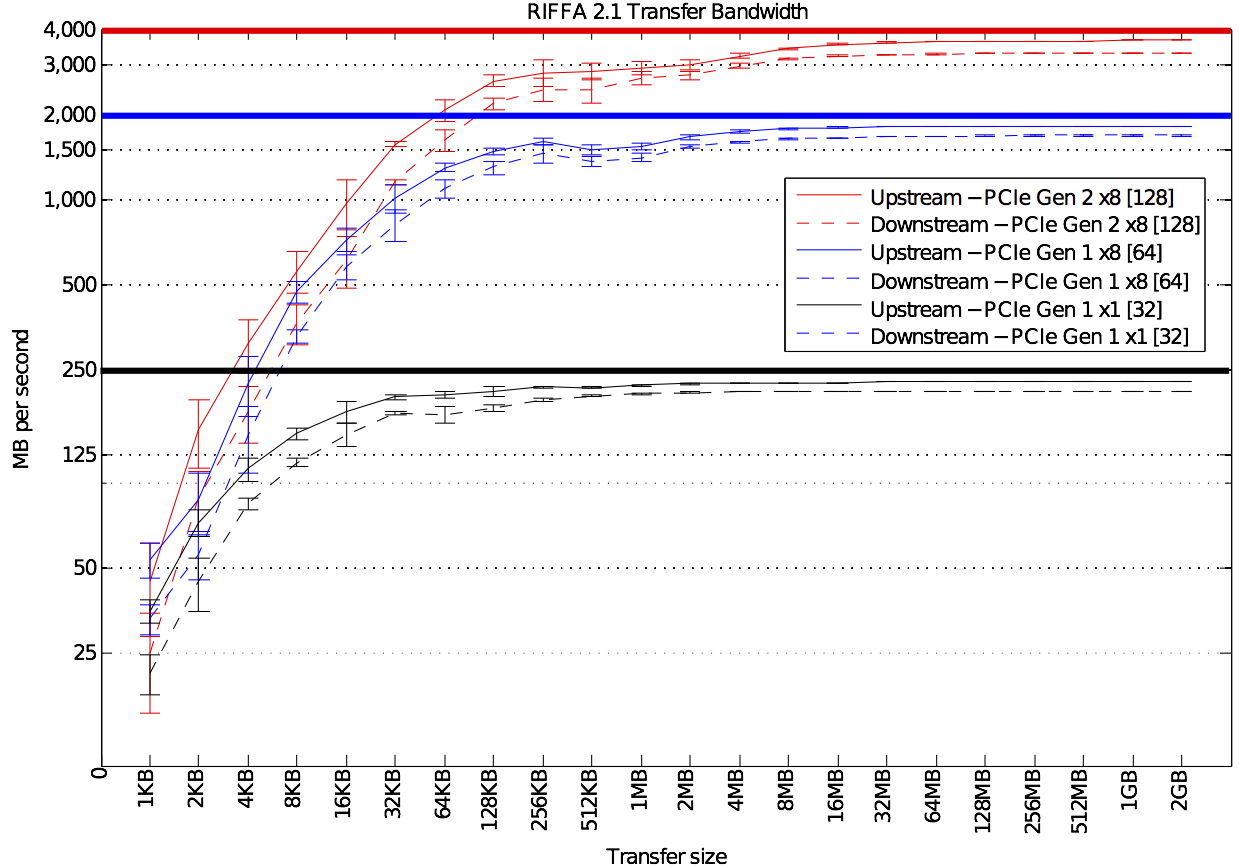
\includegraphics[width=300px,center]{bw_sg_2_1_maxs.png}
  \caption{Graph of Bandwidth vs Transfer Size}
  \label{Fig:RIFFA:Performance}
\end{figure}

RIFFA \RIFFAVer~is significantly more efficient than its predecesor RIFFA
1.0. RIFFA \RIFFAVer~is able to saturate the PCIe link for nearly all link
configurations supported. Figure~\ref{Fig:RIFFA:Performance} shows the
performance of designs using the 32 bit, 64 bit, and 128 bit interfaces. The
colored bands show the bandwidth region between the theoretical maximum and the
maximum achievable. PCIe Gen 1 and 2 use 8 bit / 10 bit encoding which limits
the maximum achievable bandwidth to 80\% of the theoretical. Our experiments
show that RIFFA can achieve 80\% of the theoretical bandwidth in nearly all
cases. The 128 bit interface achieves 76\% of the theoretical maximum.

If you are using RIFFA on a new platform not listed above let us know and we’ll
help you out!

%\pagebreak
\section{Licensing}

Copyright (c) 2016, The Regents of the University of California All rights
reserved.

Redistribution and use in source and binary forms, with or without modification,
are permitted provided that the following conditions are met:

\begin{itemize}
    \item Redistributions of source code must retain the above copyright
      notice, this list of conditions and the following disclaimer.

    \item Redistributions in binary form must reproduce the above
      copyright notice, this list of conditions and the following
      disclaimer in the documentation and/or other materials provided
      with the distribution.

    \item Neither the name of The Regents of the University of California
      nor the names of its contributors may be used to endorse or
      promote products derived from this software without specific
      prior written permission.
\end{itemize}

THIS SOFTWARE IS PROVIDED BY THE COPYRIGHT HOLDERS AND CONTRIBUTORS ``AS IS''
AND ANY EXPRESS OR IMPLIED WARRANTIES, INCLUDING, BUT NOT LIMITED TO, THE
IMPLIED WARRANTIES OF MERCHANTABILITY AND FITNESS FOR A PARTICULAR PURPOSE ARE
DISCLAIMED. IN NO EVENT SHALL REGENTS OF THE UNIVERSITY OF CALIFORNIA BE LIABLE
FOR ANY DIRECT, INDIRECT, INCIDENTAL, SPECIAL, EXEMPLARY, OR CONSEQUENTIAL
DAMAGES (INCLUDING, BUT NOT LIMITED TO, PROCUREMENT OF SUBSTITUTE GOODS OR
SERVICES; LOSS OF USE, DATA, OR PROFITS; OR BUSINESS INTERRUPTION) HOWEVER
CAUSED AND ON ANY THEORY OF LIABILITY, WHETHER IN CONTRACT, STRICT LIABILITY, OR
TORT (INCLUDING NEGLIGENCE OR OTHERWISE) ARISING IN ANY WAY OUT OF THE USE OF
THIS SOFTWARE, EVEN IF ADVISED OF THE POSSIBILITY OF SUCH DAMAGE.


\pagebreak
\chapter{Getting Started}
\section{Development Board Support in RIFFA \RIFFAVer}
RIFFA \RIFFAVer~supports:
\begin{itemize}
\item The VC707, ZC706 and similar boards with the Xilinx IP Core 7-Series
  Integrated Block for PCI Express. Example designs for the VC707 and ZC706
  boards are provided, and contain this core. The current distribution supports
  all 64-bit interfaces for these devices, with 128-bit support coming soon
  after the initial release. (Support for the 128-bit interface is in RIFFA 2.1,
  but is temporarily mising due to changes)
\item The VC709 board and similar boards with the Xilinx IP Gen3 Integrated
  Block for PCI Express. Example designs for the VC709 are provided, and contain
  this core. The current distribution supports all 64-bit and 128-bit AXI
  interfaces. 256-bit (PCIe Gen3 x8) support is planned for a later date.
\item The DE5-Net board and similar boards with the Stratix V, Cyclone V, and
  Arria V, Hard IP for PCI express (Avalon Streaming Interface). Example designs
  for the DE5-net board are provided, and contain the Stratix V version of this
  core. The current distribution supports all 64-bit and 128-bit Avalon
  Streaming interfaces.
\item The DE4 and similar boards with the IP Compiler for PCI Express Core,
  supporting Stratix IV, Cyclone IV and Arria II devices. Example designs for
  the DE4 board are provided. The current distribution supports all 64-bit and
  128-bit Avalon Streaming interfaces.
\end{itemize}
\section{Understanding this User Guide}
In this user guide, we use the following conventions:
\begin{center}
  \begin{tabular}{ | l | l |}
    \hline
    Object & Example \\ \hline
    Directories and Paths & \Directory{RIFFA \RIFFAVer/source/fpga/riffa}  \\ \hline
    Xilinx Specific Content & \Xilinx{vc709} \\ \hline
    Altera Specific Content & \Altera{de5} \\ \hline
    Configuration Setting & \ConfigSetting{Number of Lanes} \\ \hline
    Terminal Command, Code Snippet & \TermCmd{echo ``Hello World''}\\ \hline
    RIFFA Parameter & \RIFFAParameter{C\_NUM\_CHNL}\\\hline
  \end{tabular}
\end{center}

\section{Decoding What's Provided}
\label{Sec:Intro:Decoding}
Fig~\ref{Fig:RIFFA:DirStructure} shows the directory hierarchy of RIFFA. This
instruction manual uses this directory tree when specifying all directory paths.

The \Directory{RIFFA \RIFFAVer/source/fpga/} contains a directory for each board
we have tested for the current distribution:\Altera{de5, de4}, \Xilinx{VC709,
  VC707, ZC706}. Each board directory has several example project directories
(e.g. \Altera{DE5Gen1x8If64} and \Xilinx{VC709\_Gen1x8If64}). Each example
project directory has 5 sub-directories:
\begin{itemize}
\item \Directory{prj/} contains all of the project files (\Altera{.qsf,.qpf}, \Xilinx{.xpr}).
\item \Directory{ip/} contains all of the ip files (\Altera{.qsys}, \Xilinx{.xci}) generated for the project, when permitted by licensing agreements.
\item \Directory{bit/} contains the example programming file for the corresponding FPGA example design. \Altera{Quartus} and \Xilinx{Vivado} do not modify this programming (\Altera{.sof}, \Xilinx{.bit}).
\item \Directory{constr/} contains the user constraint files (\Altera{.sdc}, \Xilinx{.xdc}).
\item \Directory{hdl/} contains any example-project specific Verilog files, such as the project top level file.
\end{itemize}

\begin{figure}[H]
  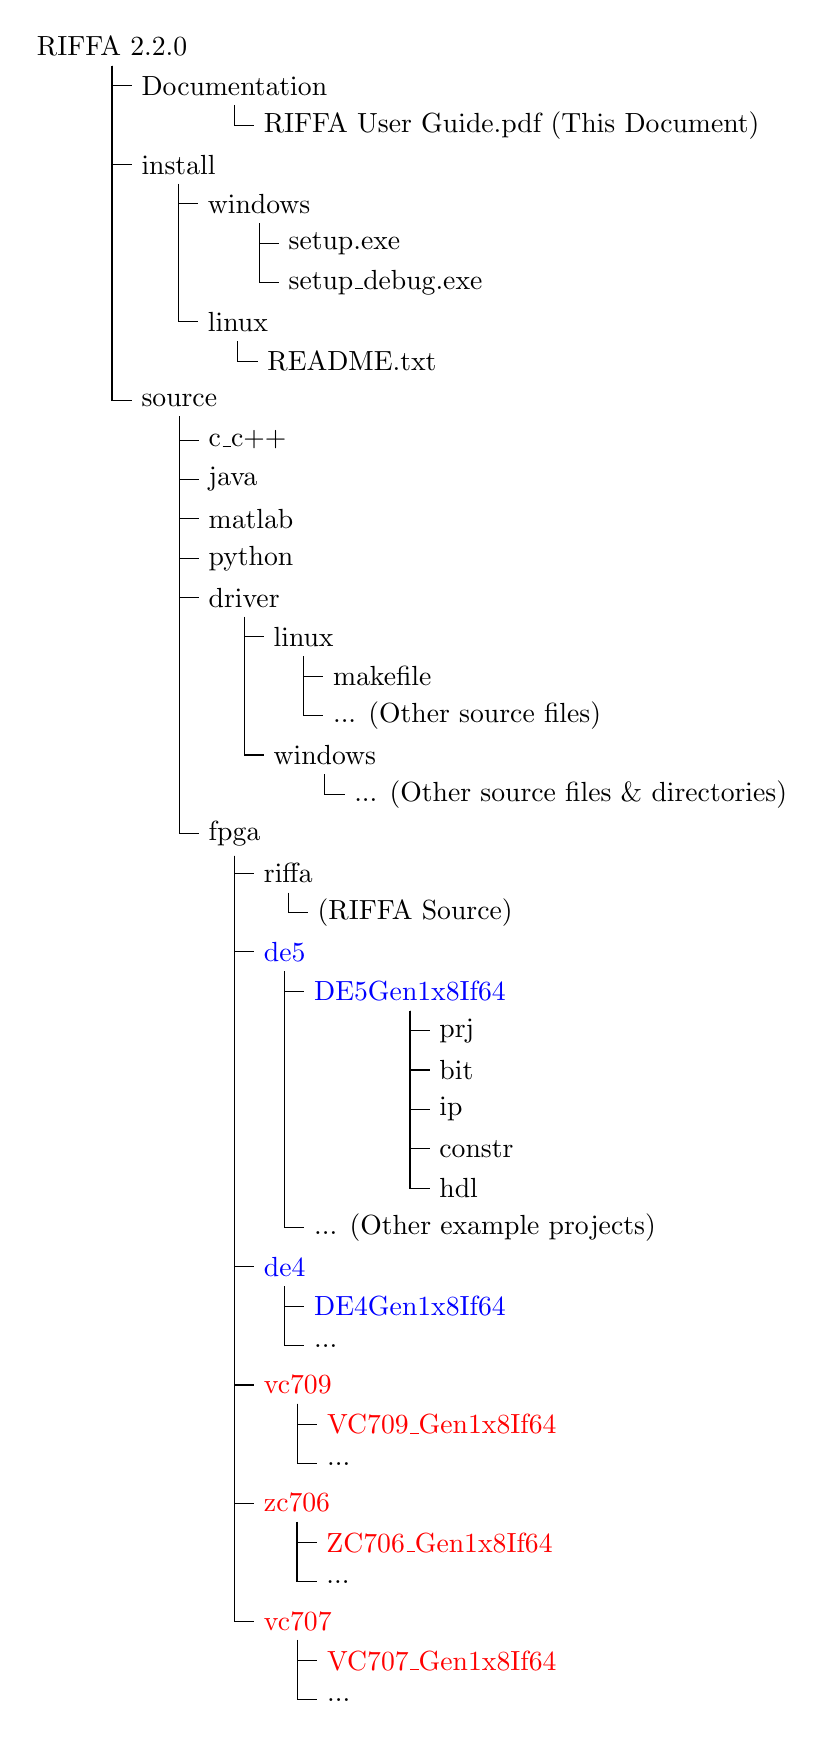
\begin{tikzpicture}[dirtree]
    \node {RIFFA \RIFFAVer}
    child { node {Documentation}
      child { node {RIFFA User Guide.pdf (This Document)} }
    }
    child { node {install}
      child { node {windows}
        child{ node {setup.exe}}
        child{ node {setup\_debug.exe}}
      }
      child { node {linux}
        child{ node {README.txt}}
      }
    }
    child { node {source}
      child { node {c\_c++} }
      child { node {java} }
      child { node {matlab} }
      child { node {python} }
      child { node {driver}
        child { node {linux}
          child{ node {makefile}}
          child{ node {... (Other source files)}}
        }
        child { node {windows}
          child{ node {... (Other source files \& directories)}}
        }
      }
      child { node{fpga}
        child { node{riffa}
          child {node{(RIFFA Source)}}
        }
        child { node{\Altera{de5}}
          child {node{\Altera{DE5Gen1x8If64}}
            child{node{prj}}
            child{node{bit}}
            child{node{ip}}
            child{node{constr}}
            child{node{hdl}}
          }
          child {node{... (Other example projects)}}
        }
        child { node{\Altera{de4}}
          child {node{\Altera{DE4Gen1x8If64}}}
          child {node{...}}
        }
        child { node{\Xilinx{vc709}}
          child {node{\Xilinx{VC709\_Gen1x8If64}}}
          child {node{...}}
        }
        child { node{\Xilinx{zc706}}
          child {node{\Xilinx{ZC706\_Gen1x8If64}}}
          child {node{...}}
        }
        child { node{\Xilinx{vc707}}
          child {node{\Xilinx{VC707\_Gen1x8If64}}}
          child {node{...}}
        }
      }
    };
  \end{tikzpicture}
  \caption{Directory hierarchy of the RIFFA \RIFFAVer~distribution} \label{Fig:RIFFA:DirStructure}
\end{figure}

\section{Release Notes}
\subsection{Version 2.2.0}
\begin{itemize}
\item Added: Support for the new Gen3 Integrated Block for PCIe Express, and the VC709 Development board.
\item Added: ZC706 Example Designs
\item Changed: Xilinx example project packaging. All Xilinx Virtex 7 projects are now click-to-compile, and come with instantiated IP.
\item Re-wrote and refactored: Various parts of the TX and RX engines to maximize code reuse between different vendors and PCIe endpoint implementations
\item Fixed: A bug in the Linux Driver that prevented compilation on older kernels
\item Fixed: A bug in the Windows Driver that prevented repeated small transfers.
\end{itemize}
\subsection{Version 2.1.0}
\begin{itemize}

\item Added reorder\_queue and updated many rx/tx engine and channel modules that 
  use it.
\item Added parameters for number of tags to use and max payload length for sizing 
  RAM for reorder\_queue.
\item Fixed: Bug in the riffa\_driver.c, too few circular buffer elements.
\item Fixed: Bug in the riffa\_driver.c, bad order in which interrupt vector bits 
  were processed. Can cause deadlock in heavy use situations.
\item Fixed: Bug in the tx\_port\_writer.v, maxlen did not start with a value of 1.
  Can cause deadlock behavior on second transfer.
\item Fixed: Bug in the rx\_port\_reader.v, added delay to allow FIFO flush to 
  propagate.
\item Fixed: Bug in rx\_port\_xxx.v, changed to use FWFT FIFO instead of existing 
  logic that could cause CHNL\_RX\_DATA\_VALID to drop for a cycle after CHNL\_RX 
  dropped even when there is still data in the FIFO. Can cause premature 
  transmission termination.
\item Changed rx\_port\_channel\_gate.v to use FWFT FIFO.
\item Removed unused signal from rx\_port\_requester\_mux.v.
\item Fixed: Typo/bug that would attempt to change state within 
  tx\_port\_monitor\_xxx.v.
\item Added flow control for receive credits to avoid over driving upstream transactions
  (applies to Altera devices).
\end{itemize}

\subsection{Version 2.0.2}
\begin{itemize}

\item Fixed: Bug in Windows and Linux drivers that could report data sent/received 
  before such data was confirmed.
\item Fixed: Updated common functions to avoid assigning input values.
\item Fixed: FIFO overflow error causing data corruption in tx\_engine\_upper and
  breaking the Xilinx Endpoint.
\item Fixed: Missing default cases in rx\_port\_reader, sg\_list\_requester, 
  tx\_engine\_upper, and tx\_port\_writer.
\item Fixed: Bug in tx\_engine\_lower\_128 corrupting s\_axis\_tx\_tkeep, causing Xilinx
  PCIe endpoint core to shut down.
\item Fixed: Bug in tx\_engine\_upper\_128 causing incomplete TX data timeouts.
\item Changed rx\_engine to not block on nonposted TLPs. They're added to a FIFO and
  serviced in order. 
\item Reset rx\_port FIFOs before a receive transaction to avoid data corruption from
  replayed TLPs.
\end{itemize}

\subsection{Version 2.0.1}

\begin{itemize}
\item RIFFA 2.0.1 is a general release. This means we've tested it in a number of
  ways. Please let us know if you encounter a bug. 
\item Neither the HDL nor the drivers from RIFFA 2.0.1 are backwards compatible with
  the components of any previous release of RIFFA.
\item RIFFA 2.0.1 consumes more resources than 2.0 beta. This is because 2.0.1 was
  rewritten to support scatter gather DMA, higher bandwidth, and appreciably 
  more signal registering. The additional registering was included to help meet 
  timing constraints. 
\item The Windows driver is supported on Windows 7 32/64. Other Windows versions 
  can be supported. The driver simply needs to be built for that target.
\item Debugging on Windows is difficult because there exists no system log file.
  Driver log messages are visible only to an attached kernel debugger. So to see
  any messages you'll need the Windows Development Kit debugger (WinDbg) or a 
  small utility called DbgView. DbgView is a standalone kernel debug viewer that
\item   http://technet.microsoft.com/ens/sysinternals/bb896647.aspx
  Run DbgView with administrator privileges and be sure to enable the following
  capture options: Capture Kernel, Capture Events, and Capture Verbose Kernel 
  Output.
\item The Linux driver is supported on kernel version 2.6.27+. 
\item The Java bindings make use of a native library (in order to connect Java JNI
  to the native library). Libraries for Linux and Windows for both 32/64 bit 
  platforms have been compiled and included in the riffa.jar.
\item Removed the CHNL\_RX\_ERR signal from the channel interface. Error handling now
  ends the transaction gracefully. Errors can be easily detected by comparing
  the number of words received to the CHNL\_RX\_LEN amount. An error will cause
  CHNL\_RX will go low prematurely and not provide the advertised amount of data.
\item Fixed: Bug in sg\_list\_requester which could cause an unbounded TLP request.
\item Fixed: Bug in tx\_port\_buffer\_128 which could stall the TX transaction.
\end{itemize}
\section{Errata}
While we have extensively tested the current distribution, we are human and
cannot eliminate all bugs in our distribution. As a general rule of thumb, if
you find yourself delving into the RIFFA code, you have gone too far. Contact us
if you need additional assistance!

See the following notes for issues we are currently tracking:

\subsection{Windows}
\subsection{Linux}
No open issues
\subsection{Altera}
\textbf{Issue 1: Inexplicable DE4 behavior} We are seeing inexplicable behavior
on the DE4 boards. In particular, this affects both upstream and downstream data
transfers on the Gen2 128-bit interface. In the channel tester, this problem
manifests as an incorrect number of words recieved, and incorrrect data sent.

\textbf{Issue 2: DE4 Designs intermittently fail timing} Particularly on the
128-bit interface. Working to fix.

\textbf{Issue 3: No support for the 256-bit, Gen3x8 Interface} Coming soon...
\subsection{Xilinx (Classic)}

\textbf{Issue 1: Missing example designs for ML605} There is no disadvantage to
using RIFFA 2.1.0 until we return support in a future distribution.

\textbf{Issue 2: Missing example design for Spartan 6 LXT Development board} The
32-bit interface support has been removed from RIFFA 2.2 and may be added back
in the future. Please use RIFFA 2.1 in the meantime

\subsection{Xilinx (Ultrascale)}
\textbf{Issue 1: No support for the 256-bit, Gen3x8 Interface} Coming soon...

\pagebreak

\chapter{Installing the RIFFA driver}
\label{Sec:RIFFA:Installation}
\section{Linux}
To install the RIFFA driver in linux, you must build it against your installed
version of the Linux kernel. RIFFA \RIFFAVer~comes with a makefile that will
install the necessar linux kernel headers and the driver. This makefile will
also build and install the C/C++ native library. To install RIFFA \RIFFAVer~in
linux, follow these instructions:

\begin{enumerate}
\item Open a terminal in linux and navigate to the \Directory{RIFFA \RIFFAVer/source/driver/linux} directory.
\item Ensure you have the kernel headers installed, run:

  \TermCmd{sudo make setup}

  This will attempt to install the kernel headers using your system's package
  manager. You can skip this step if you've already installed the kernel headers.
\item Compile the driver and C/C++ library:

  \TermCmd{make}

  or

  \TermCmd{make debug}

  Using make debug will compile in code to output debug messages to the system log
  at runtime. These messages are useful when developing your design. However they
  pollute your system log and incur some overhead. So you may want to install the
  non-debug version after you've completed development.
\item Install the driver and library:

  \TermCmd{sudo make install}

  The system will be configured to load the driver at boot time. The C/C++ library
  will be installed in the default library path. The header files will be placed
  in the default include path. You will need to reboot after you've installed for
  the driver to be (re)loaded. 
\item If the driver is installed and there is a RIFFA \RIFFAVer~configured FPGA when the computer boots, the
  driver will detect it. Output in the system log will provide additional
  information. 
\item The C/C++ code must include the riffa.h header. An example inclusion is
  shown in Listing~\ref{Listing:RIFFA:Include}
\item When compiling (using GCC/G++, etc.) you must link with the RIFFA
  libraries using the -lriffa flag. For example, when compiling test.c from
  Listing~\ref{Listing:RIFFA:Include}:

  \TermCmd{gcc -g -c -lriffa -o test.o test.c}
\item Bindings for other languages can be installed by following the README
  files in their respective directories (See Figure~\ref{Fig:RIFFA:DirStructure}
\end{enumerate}

\section{Windows}
Currently only Windows 7 (32/64) is supported by RIFFA \RIFFAVer. In the
\Directory{RIFFA \RIFFAVer/install/windows/} subdirectory use the
provided setup.exe program to install the RIFFA driver and native C/C++
library. You can verify that RIFFA \RIFFAVer~installed correctly by checking
the installation directory in Program Files. After installation, you'll be able
to install the bindings for other languages.

The setup\_dbg.exe installer installs a driver with additional debugging output.
You can install the setup\_dbg.exe version and then later use setup.exe to
install the non-debug output version.

\begin{lstlisting}[basicstyle=\footnotesize\ttfamily,language=C,
    commentstyle=\color{red},label=Listing:RIFFA:Include,
    caption=Inclusion of the RIFFA header files in a user application,frame=single]
  #include <stdio.h>
  #include <stdlib.h>
  #include <riffa.h>
  #define BUF_SIZE (1*1024*1024)

  unsigned int buf[BUF_SIZE];

  int main(int argc, char* argv[]) {
    fpga_t * fpga;
    int fid = 0; // FPGA id
    int channel = 0; // FPGA channel

    fpga = fpga_open(fid);
    fpga_send(fpga, channel, (void *)buf, BUF_SIZE, 0, 1, 0);
    fpga_recv(fpga, channel, (void *)buf, BUF_SIZE, 0);
    fpga_close(fpga);
    return 0;
  }
\end{lstlisting}


\chapter{Compiling and using the Xilinx Example Designs}
Vivado \VivadoVer~was used in all example designs and documentation included in
this distribution. We highly recommend using \VivadoVer~and all newer versions
of the software, since we have encountered bugs in previous versions of the
Vivado (e.g. 2014.2) software. This guide assumes that the end-user has already
configured their board for PCI Express operation. See the VC709 User Guide
\footnote{http://www.xilinx.com/support/documentation/boards\_and\_kits/vc709/ug887-vc709-eval-board-v7-fpga.pdf},
VC707 User Guide
\footnote{http://www.xilinx.com/support/documentation/boards\_and\_kits/vc707/ug848-VC707-getting-started-guide.pdf}
or ZC706 User Guide
\footnote{http://www.xilinx.com/support/documentation/boards\_and\_kits/zc706/ug954-zc706-eval-board-xc7z045-ap-soc.pdf}.

While we have not tested all of the current-generation Xilinx development
boards, we are confident that they can be supported with minimal
modifications. For more information about supporting new boards, see the
sections \ref{Sec:7SeriesIntegrated:Generating} and
\ref{Sec:Gen3Integrated:Generating}. These sections cover the settings used
in the RIFFA example design IP.

The easiset way to use RIFFA is to start with one of the example designs
included in the distribution. Sections \ref{Sec:7SeriesIntegrated:ExampleDesign}
and \ref{Sec:Gen3Integrated:ExampleDesign} describe how to use and compile these
designs for the VC707 and VC709 boards respectively. These example designs are
ready to compile out of the box, and require no user IP configuration and
generation. The designs also include pre-compiled bit-files in the
\Directory{bit} directory of the example project. For advanced users, we also
describe how we generated the PCIe IP in sections
\ref{Sec:7SeriesIntegrated:Generating} and
\ref{Sec:Gen3Integrated:Generating}.

\section{Classic - 7 Series Integrated Block for PCI Express - (VC707, ZC706 and older)}  
This is a step by step guide for using RIFFA \RIFFAVer~on a Xilinx FPGA with the
7 Series Integrated Block for PCI Express Core. This core is supported on the
ZC706, and VC707 development boards, using the 64-bit and 128-bit AXI
interfaces.

\subsection{VC707 and ZC706 Example Designs}
\label{Sec:7SeriesIntegrated:ExampleDesign}
There is one VC707 example design and two ZC706 example designs in the RIFFA
\RIFFAVer~distribution. The VC707 example design folders are in \Directory{RIFFA
  \RIFFAVer/source/fpga/vc707} and the ZC706 example design folders are in
\Directory{RIFFA \RIFFAVer/source/fpga/zc706}.

\begin{enumerate}
\item Open Vivado to get the introductory screen shown in
  Figure~\ref{Fig:Vivado:WelcomeScreen}.
\item Click 'Open an Existing Project' and navigate to your RIFFA
  \RIFFAVer~directory.
\item In the RIFFA \RIFFAVer~distribution, open \Directory{RIFFA
  \RIFFAVer/source/fpga/xilinx/vc707/} or \Directory{RIFFA
  \RIFFAVer/source/fpga/zc706} and choose from one of the existing example
  design directories for your board. In the example design directory, locate the
  \Directory{prj} folder and open it. Select the .xpr file and click open. This
  will open the example project, as shown in
  Figure~\ref{Fig:7SeriesIntegrated:ExampleDesign:ProjectOpened}.
\item This project was compiled in Vivado \VivadoVer. The bit file generated can
  be used to test the FPGA system. If you are using a newer version of Vivado,
  recompile the example design or use the programming file provided.
  \begin{itemize}
  \item IP Settings are now packaged as part of the example designs! Users no
    longer need to generate IP.
  \item To recompile the example design, click the generate bitstream button in
    the top left corner as shown in
    Figure~\ref{Fig:7SeriesIntegrated:ExampleDesign:ProjectOpened}.
  \item Recompiling your design will generate a new bitfile in the Xilinx
    project. The bit file in the \Directory{bit} will not be changed.
  \end{itemize}
\item To program the FPGA, click 'Open Hardware Manager'. New bit files
  (generated by Vivado) will appear in Vivado's internal directory. An example
  bit file is provided in the example design's \Directory{bit}. Load the
  bitstream to your VC707 or ZC706 board and restart your computer.
  \begin{itemize}
  \item Before programming your FPGA, you should install the RIFFA driver. See
    Section~\ref{Sec:RIFFA:Installation}
  \end{itemize}
\item The example design uses the chnl\_tester (shown in
  Figure~\ref{Fig:Vivado:ExampleDesign:chnl_tester}, which works with
  the example software in the \Directory{source/\{C\_C++,Java,python,matlab\}}
  directories. Replace the chnl\_tester instantiation with any user logic,
  matching the RIFFA interface.
\item Recompile the design and program the FPGA Device. Changing the
  \RIFFAParameter{C\_NUM\_CHNL} will change the number of independent channel
  interfaces
\end{enumerate}
\begin{figure}
  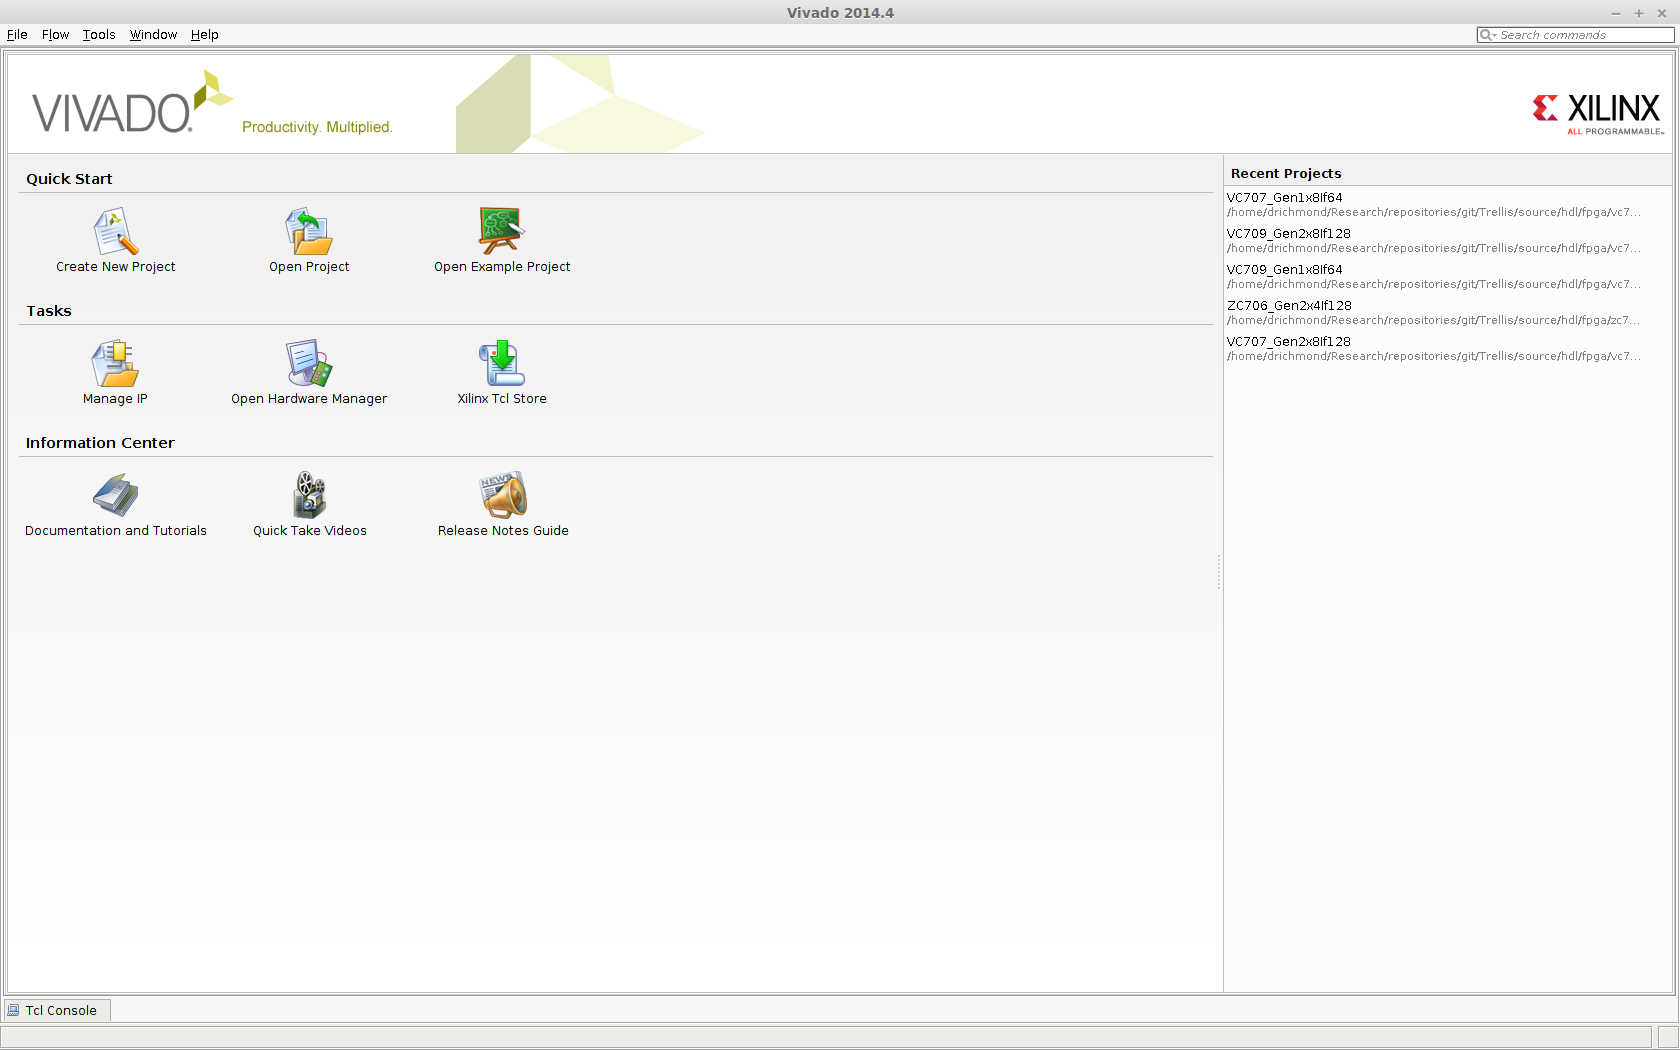
\includegraphics[width=400px,center]{VivadoWelcomeScreen.png}
  \caption{Welcome Screen for Vivado \VivadoVer}
  \label{Fig:Vivado:WelcomeScreen}
\end{figure}
\begin{figure}
  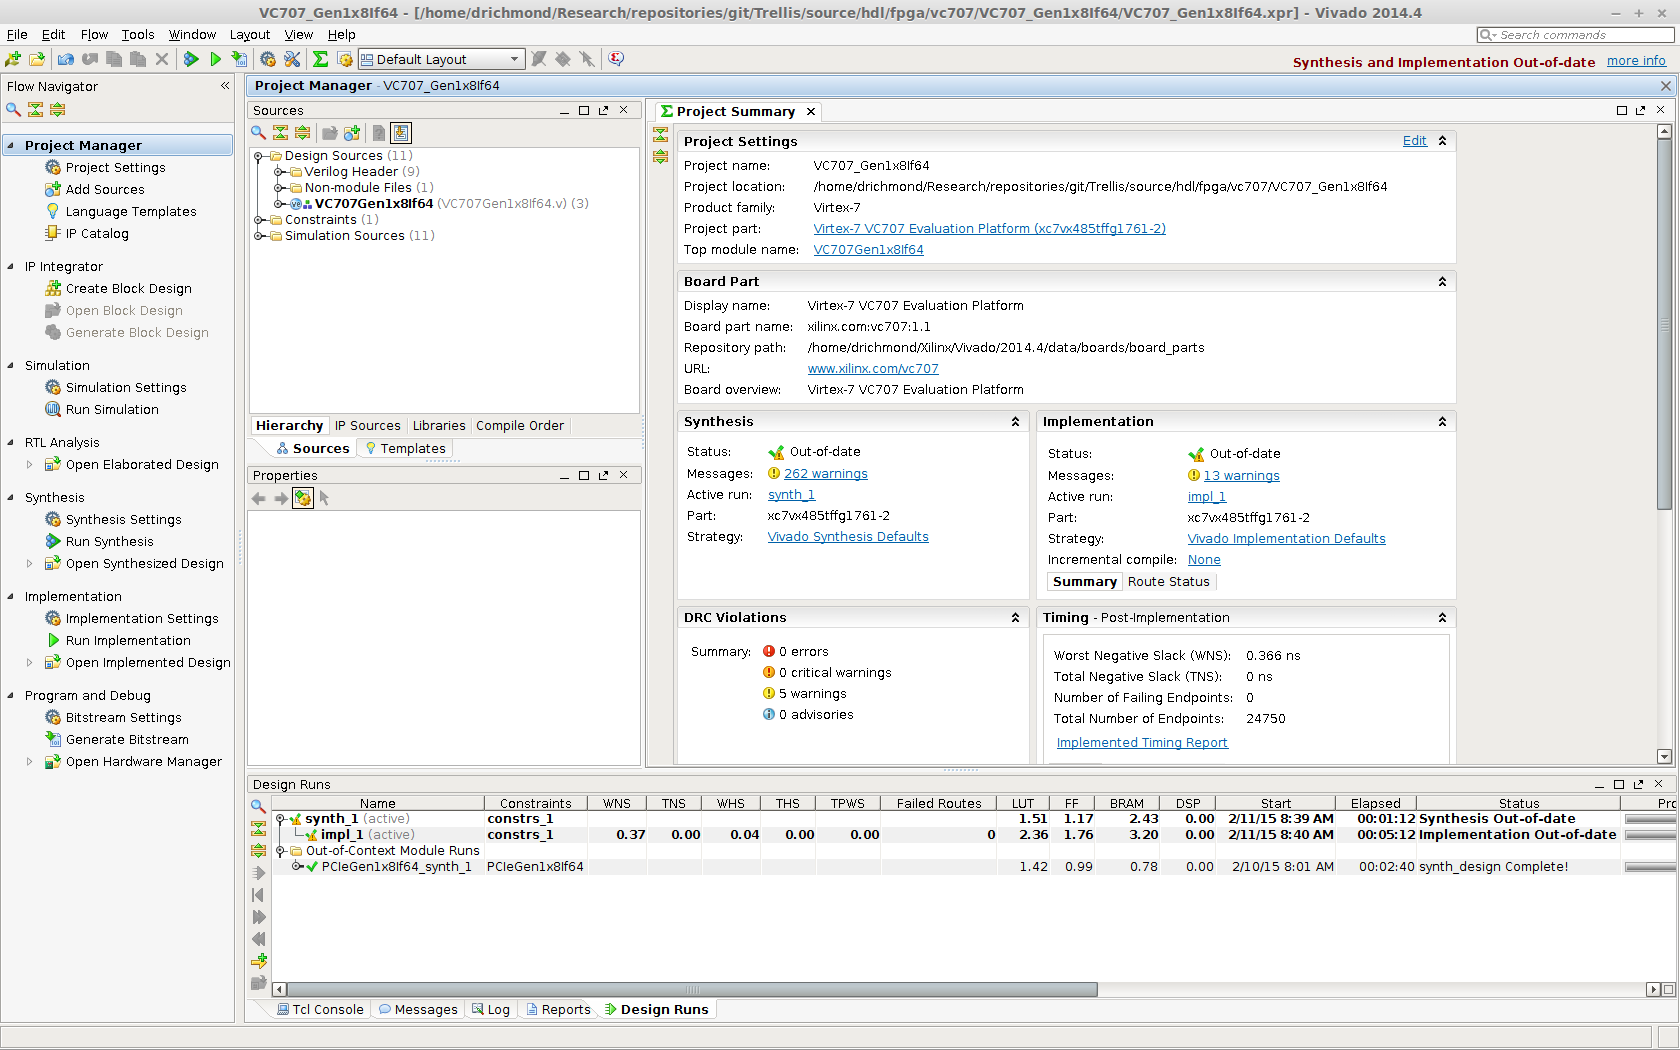
\includegraphics[width=400px,center]{7SeriesIntegratedOpenProject.png}
  \caption{Project Splash Screen for 7Series Integrated Block for PCI Express Projects}
  \label{Fig:7SeriesIntegrated:ExampleDesign:ProjectOpened}
\end{figure}
\begin{figure}
  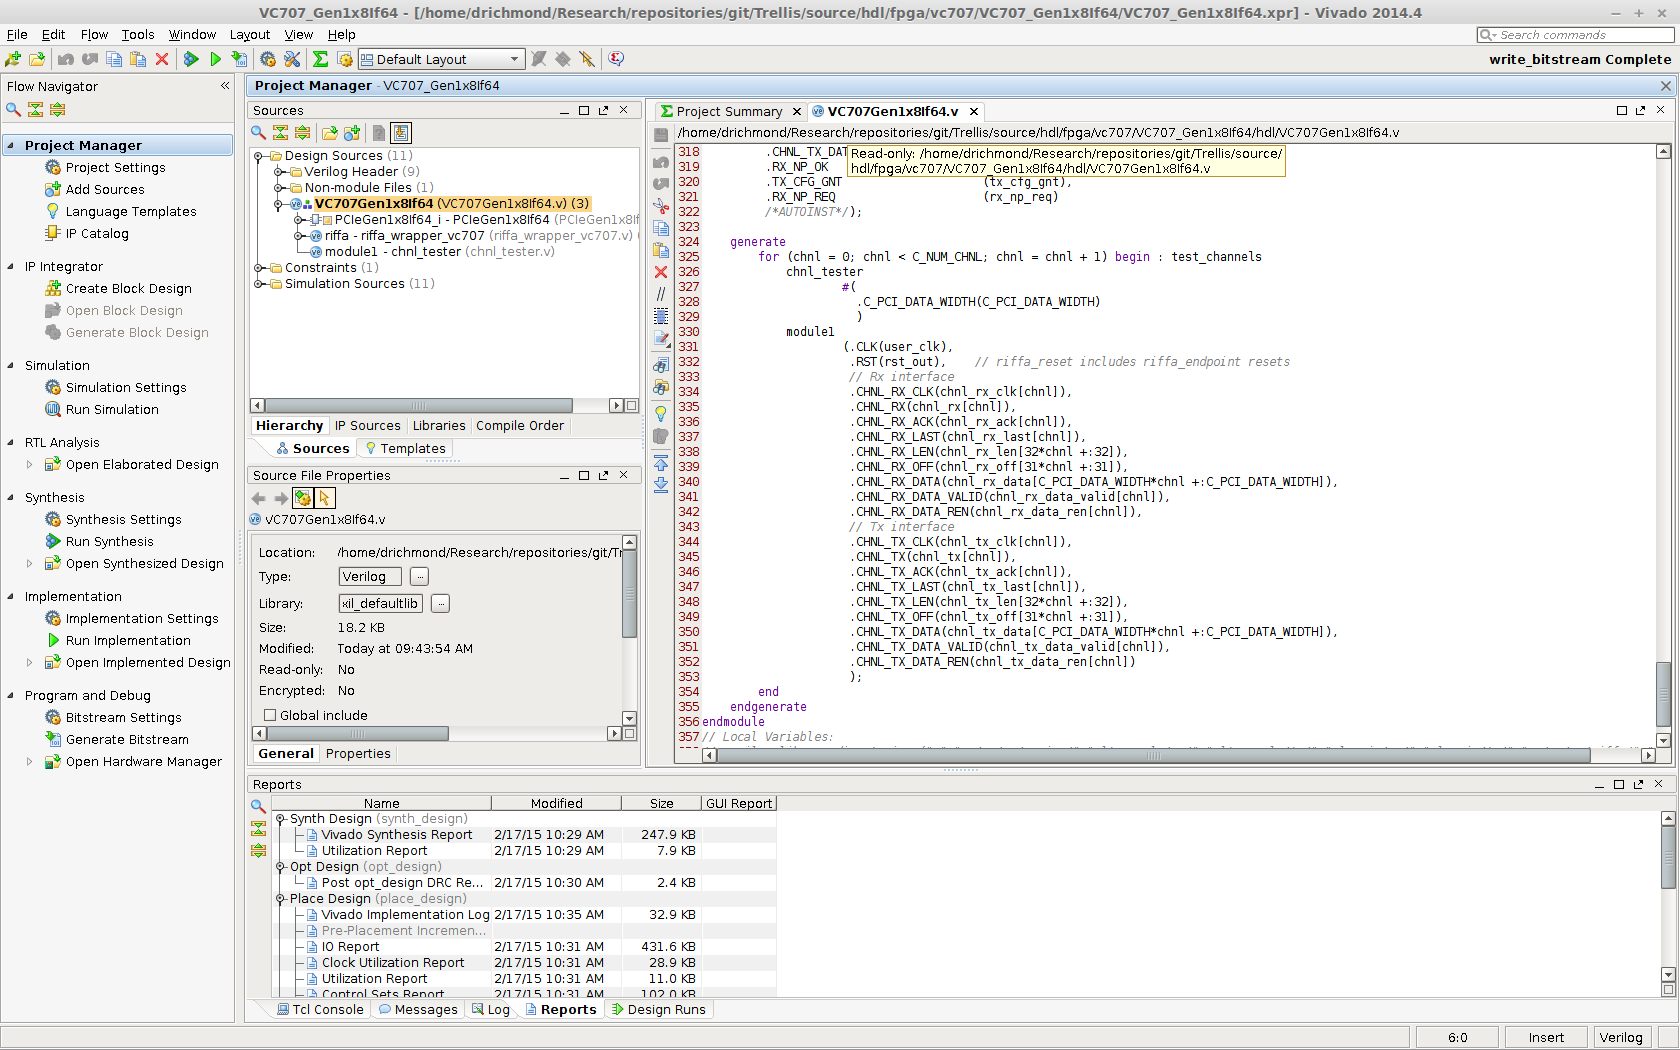
\includegraphics[width=400px,trim=500 200 200 250, clip=true,center]{VivadoChnlTesterInstantiation.png}
  \caption{Project Splash Screen for 7Series Integrated Block for PCI Express Projects}
  \label{Fig:Vivado:ExampleDesign:chnl_tester}
\end{figure}

\subsection{Generating the 7 Series Integrated Block for PCI Express}
\label{Sec:7SeriesIntegrated:Generating}
The following steps are not required for general users. See the instructions
above for how to compile RIFFA.

Alternatively, it is possible to generate the PCIe Endpoint with different
settings than those provided in the example design. Modifying the RIFFA
parameters \RIFFAParameter{C\_PCI\_DATA\_WIDTH},
\RIFFAParameter{C\_MAX\_PAYLOAD\_BYTES} and \RIFFAParameter{C\_LOG\_NUM\_TAGS},
change certain settings in the IP Core. The \RIFFAParameter{C\_NUM\_LANES} is a
parameter in the top level file of each example project. How these parameters
relate to IP core settings is highlighted in the following figures.

If the goal is to generate a RIFFA design completely from scratch, each board
directory comes with a RIFFA wrapper verilog file and instantiates a
vendor-specific translation layer. It is highly recommended to re-use these
files RIFFA wrapper when creating designs from scratch.

To generate the PCIe IP select the 7 Series Integrated Block for PCI Express
after selecting the IP Catalog shown in
Figure~\ref{Fig:7SeriesIntegrated:ExampleDesign:ProjectOpened}. This will open
the IP Customization window as shown in 
Figure~\ref{Fig:7SeriesIntegrated:Generating:7SeriesIntegratedTabBasic}
\begin{figure}[H]
  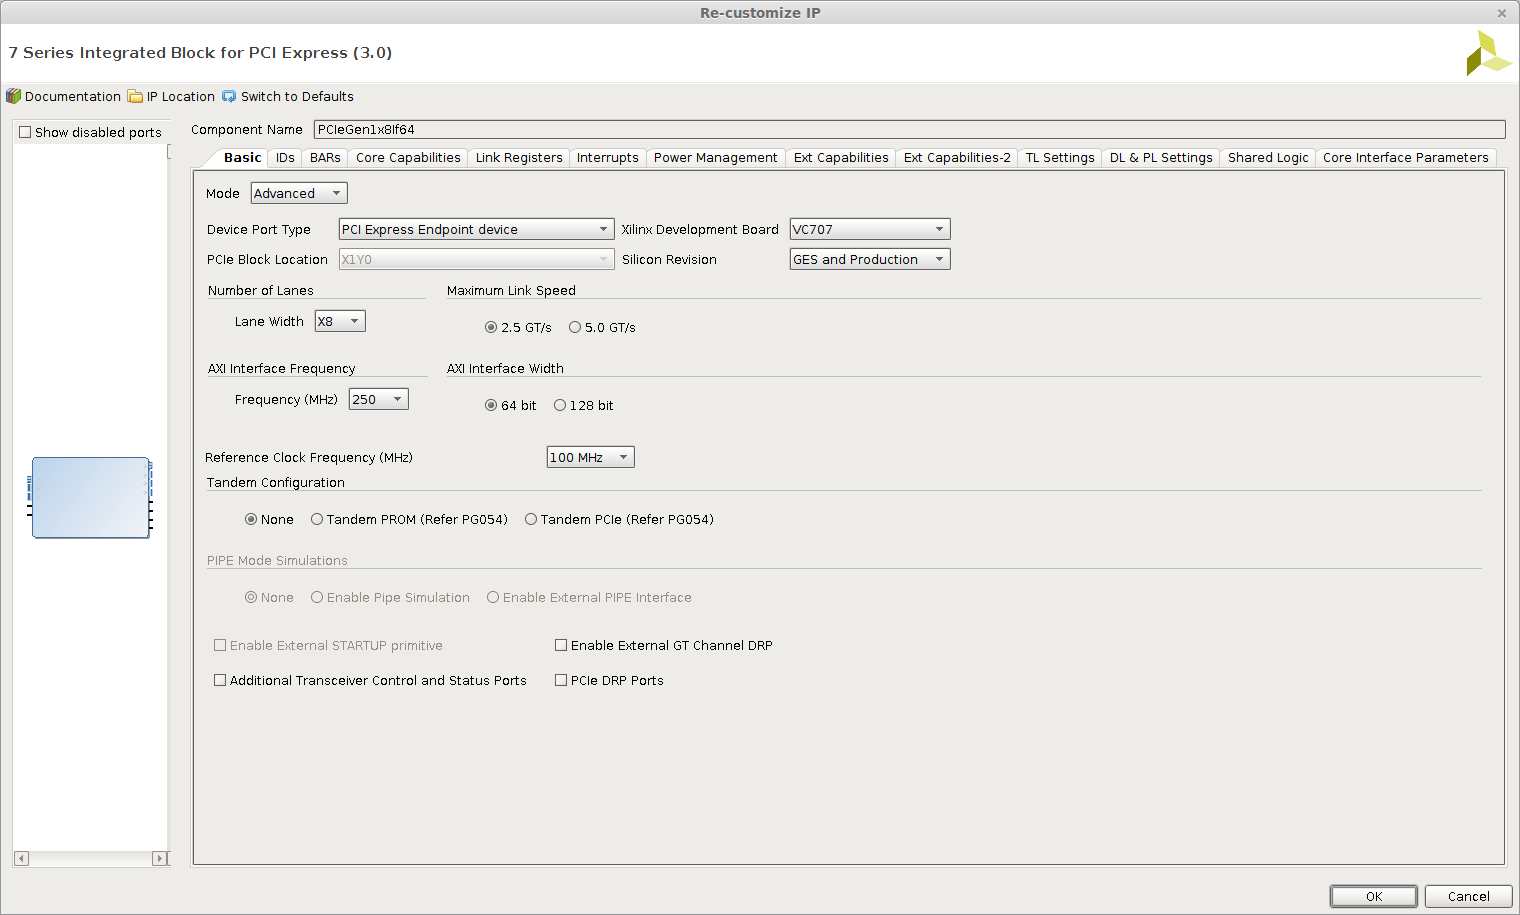
\includegraphics[width=\figurewidth,center]{7SeriesIntegratedTabBasic.png}
  \caption{Basic settings tab.}
  \label{Fig:7SeriesIntegrated:Generating:7SeriesIntegratedTabBasic}
\end{figure}
First, select \ConfigSetting{Mode} to \ConfigSetting{ADVANCED} from the drop
down menu. This will cause more tabs to appear in the bar. The following tabs
are not used during customization: Link Registers, Power Mangement,
Ext. Capabilities, Ext. Capabilities 2, TL Settings and DL/PL Settings.

In Figure~\ref{Fig:7SeriesIntegrated:Generating:7SeriesIntegratedTabBasic} , we
have set the \ConfigSetting{Xilinx Development Board} to \ConfigSetting{VC707},
selected the PCIe Gen1 rate \ConfigSetting{2.5 GT/s}, and a \ConfigSetting{Lane
  Width} of \ConfigSetting{8} (\RIFFAParameter{C\_NUM\_LANES} = 8). We have
chosen to set the \ConfigSetting{AXI Interface Width} to \ConfigSetting{64-bits}
(\RIFFAParameter{C\_PCI\_DATA\_WIDTH} = 64). The choice of Link Rate, Lanes, and
Interface Width will allow different AXI Interface Frequencies to be
selected. The RIFFA core will run at this clock frequency, but the user logic
can run at whatever frequency it desires.

Optional: Set the Component Name of the PCI Express block, and the IP
Location. In our example projects, we use the name template
PCIeGen\textbf{W}x\textbf{Y}If\textbf{Z} where \textbf{W} is the PCI Express
Version (\ConfigSetting{Link Speed} in
Figure~\ref{Fig:7SeriesIntegrated:Generating:7SeriesIntegratedTabBasic}),
\textbf{Y} is the lane width, and \textbf{Z} is the AXI interface width.  The IP
location is the \Directory{ip} directory in the example project.

\begin{figure}[H]
  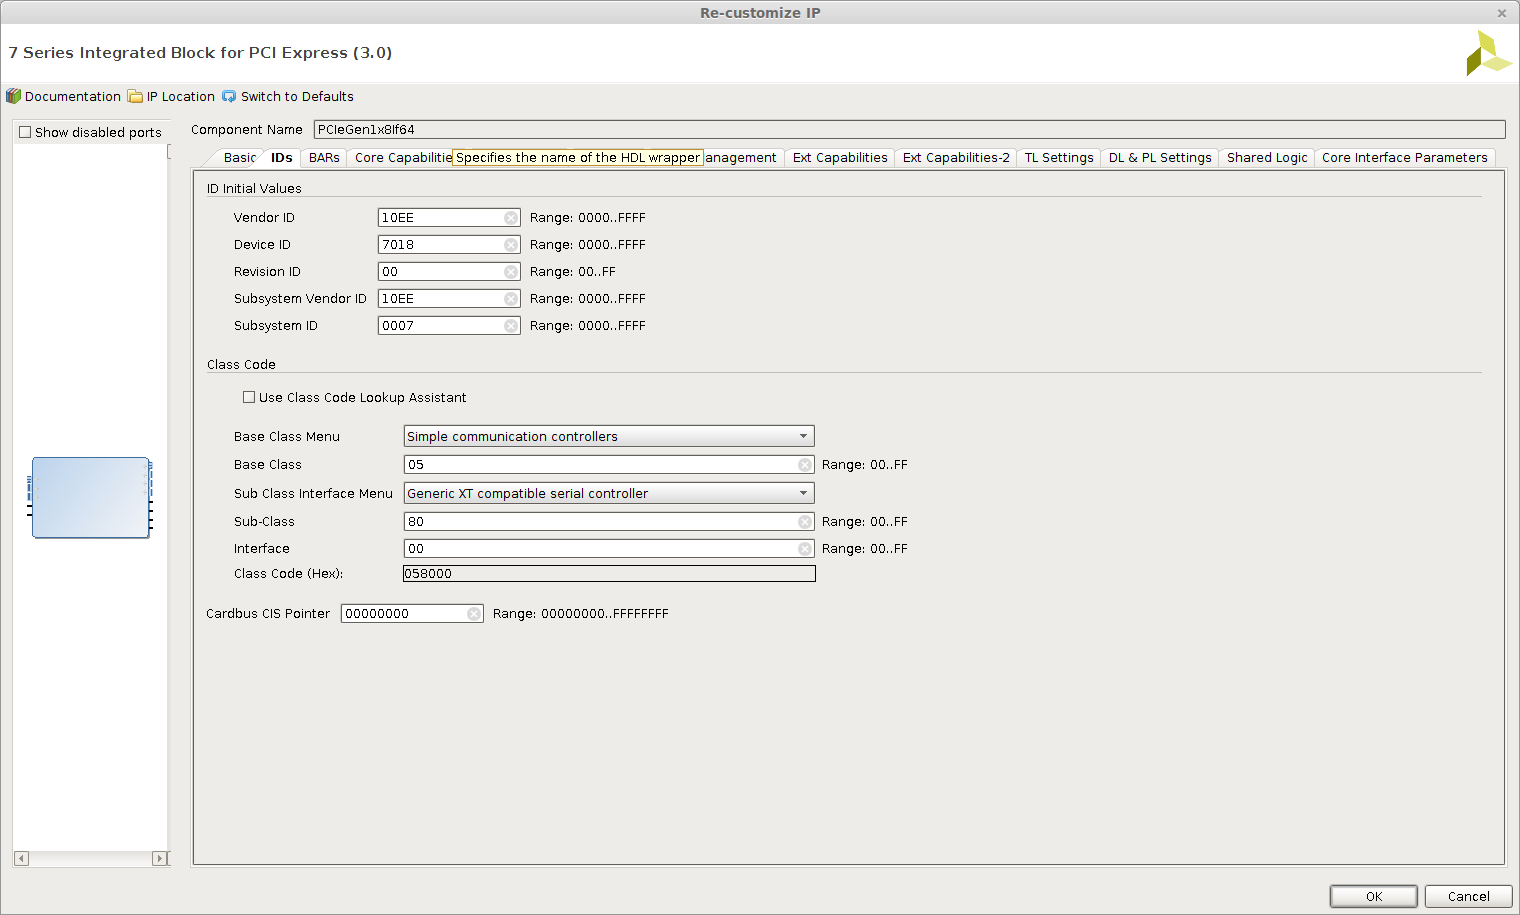
\includegraphics[width=350px,center]{7SeriesIntegratedTabIDs.png}
  \caption{PCI Express ID Tab.}
  \label{Fig:7SeriesIntegrated:Generating:7SeriesIntegratedTabIDs}
\end{figure}
The tab in Figure~\ref{Fig:7SeriesIntegrated:Generating:7SeriesIntegratedTabIDs}
is optional. Setting the Device ID may assist in identifying different FPGAs in
a multi-FPGA system. The other options, specifically the Vendor ID, must remain
the same.

\begin{figure}[H]
  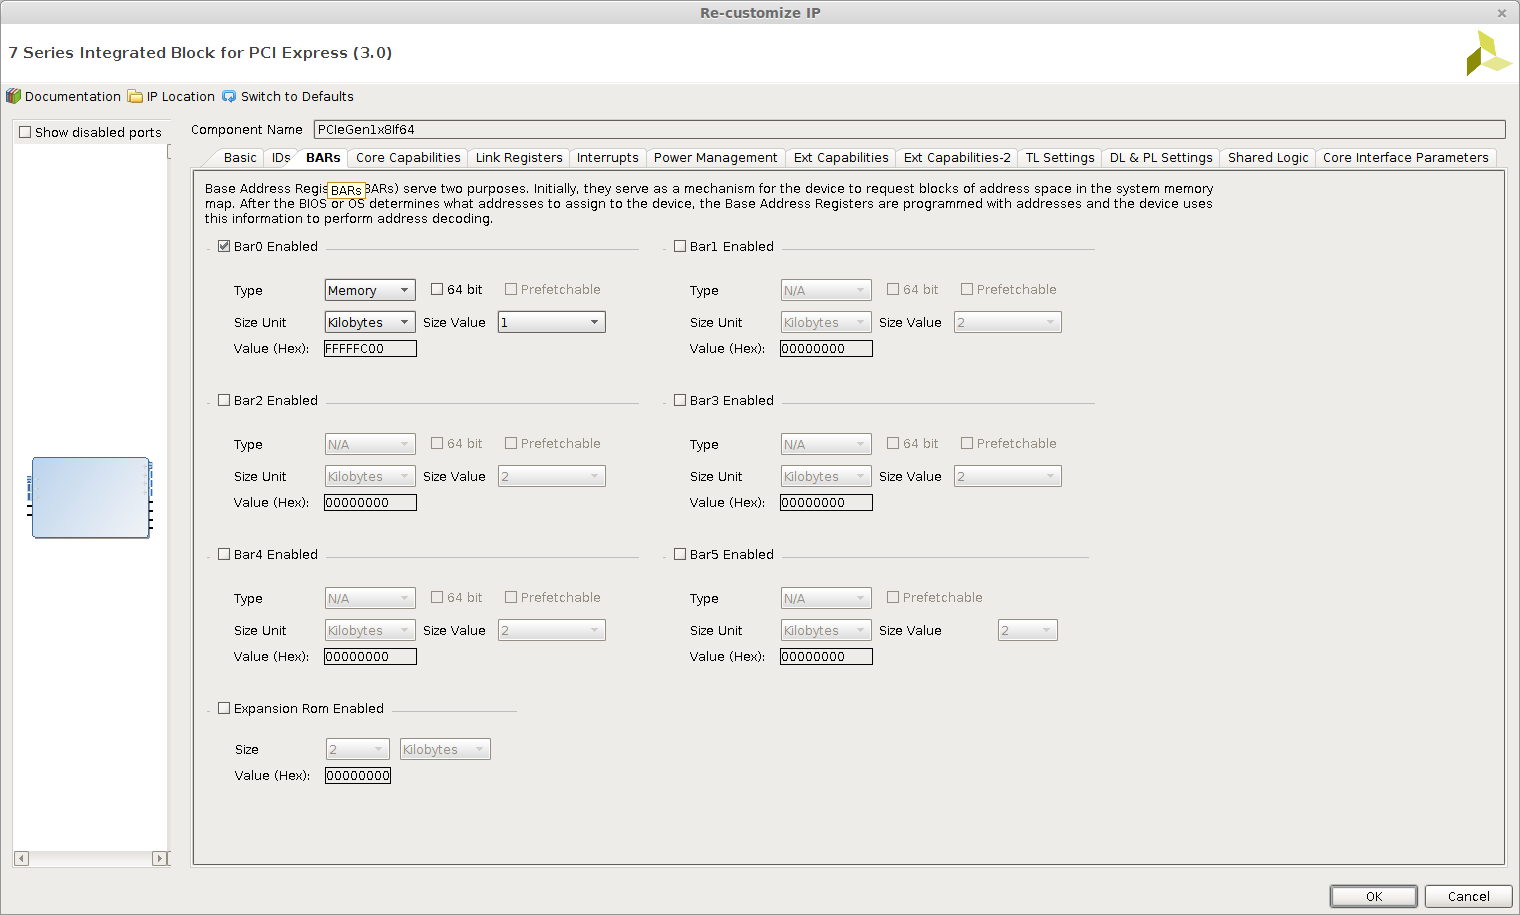
\includegraphics[width=350px,center]{7SeriesIntegratedTabBARs.png}
  \caption{PCI Express Base Address Register (BAR) ID Tab.}
  \label{Fig:7SeriesIntegrated:Generating:7SeriesIntegratedTabBARs}
\end{figure}
The tab in
Figure~\ref{Fig:7SeriesIntegrated:Generating:7SeriesIntegratedTabBARs} must be
configured so that BAR0 is \ConfigSetting{enabled} (checked). Set the
\ConfigSetting{Type} to \ConfigSetting{Memory}, and \ConfigSetting{Unit}
\ConfigSetting{Kilobyte}, and \ConfigSetting{Size Value} to \ConfigSetting{1}
from the dropdown menus. If these values are not set correctly the RIFFA driver
will not recognize the FPGA device.

\begin{figure}[H]
  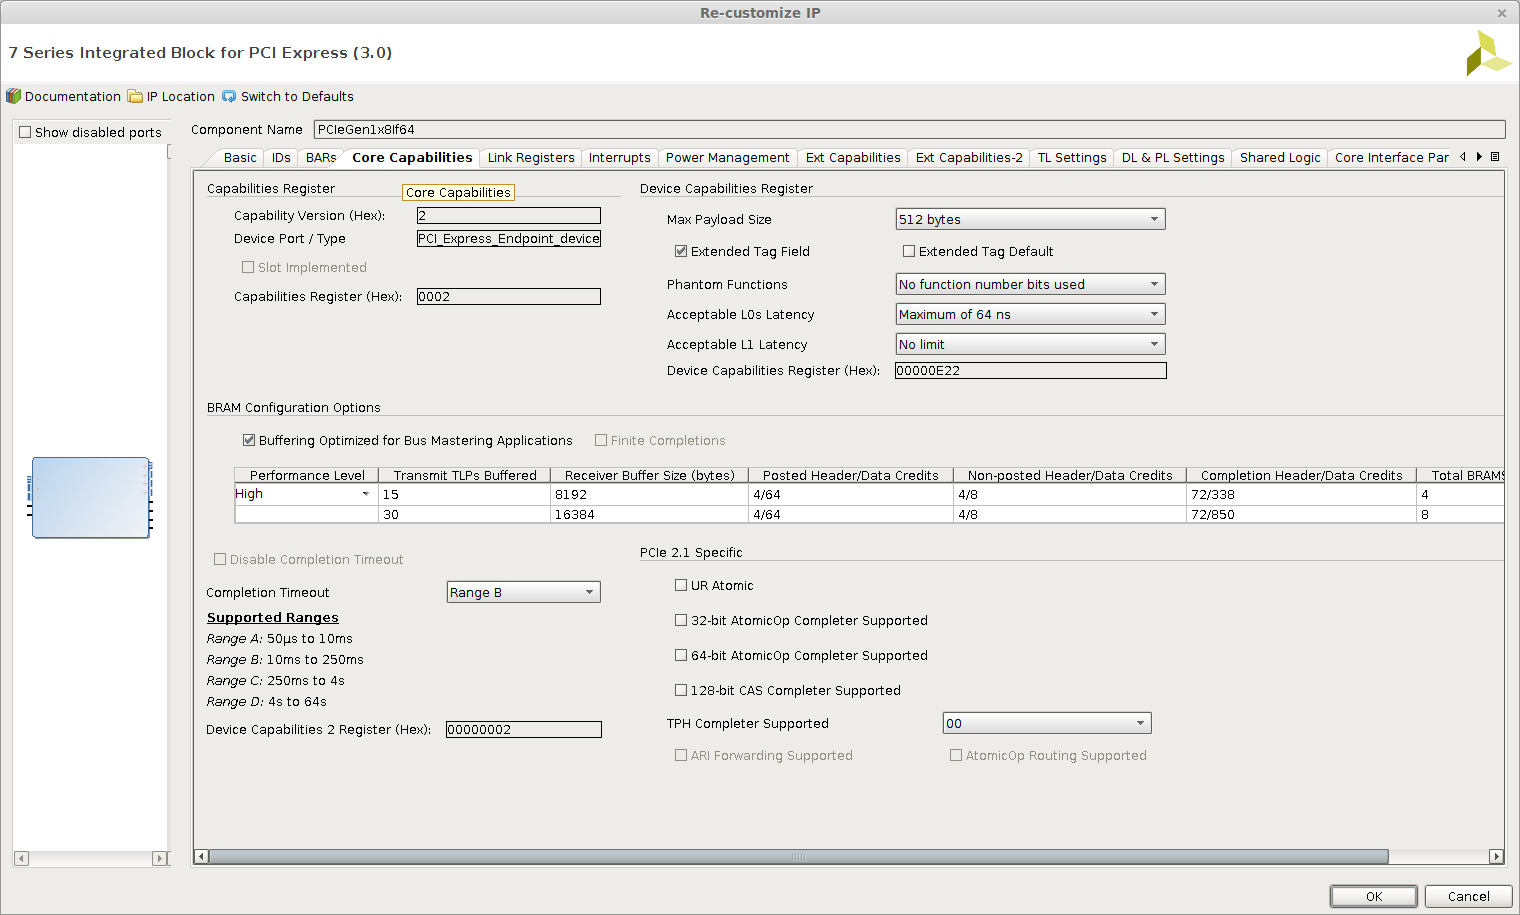
\includegraphics[width=350px,center]{7SeriesIntegratedTabCapabilities.png}
  \caption{PCI Express Capabilities Tab.}
  \label{Fig:7SeriesIntegrated:Generating:7SeriesIntegratedTabCapabilities}
\end{figure}
In this tab select the boxes \ConfigSetting{Buffering Optimized for Bus
  Mastering Applications} and \ConfigSetting{Extended Tag Field}. If the
\ConfigSetting{Extended Tag Field} is selected
\RIFFAParameter{C\_LOG\_NUM\_TAGS} = 8, otherwise
\RIFFAParameter{C\_LOG\_NUM\_TAGS} = 5. Select the \ConfigSetting{Maximum
  Payload Size} from the dropdown menu. Use this to set the RIFFA
\RIFFAParameter{C\_MAX\_PAYLOAD\_BYTES} parameter.

Note: Maximum Payload sizes are typically set by the BIOS, and 256 bytes seems
to be standard. RIFFA will default to the minimum of
\RIFFAParameter{C\_MAX\_PAYLOAD\_SIZE} and the setting in your BIOS. Unless your
BIOS is modified, or can support substantially larger packets, there will be no
performance benefit to increasing the payload size. Increasing the maximum
payload size will increase the resources consumed.

% \begin{figure}[H]
%   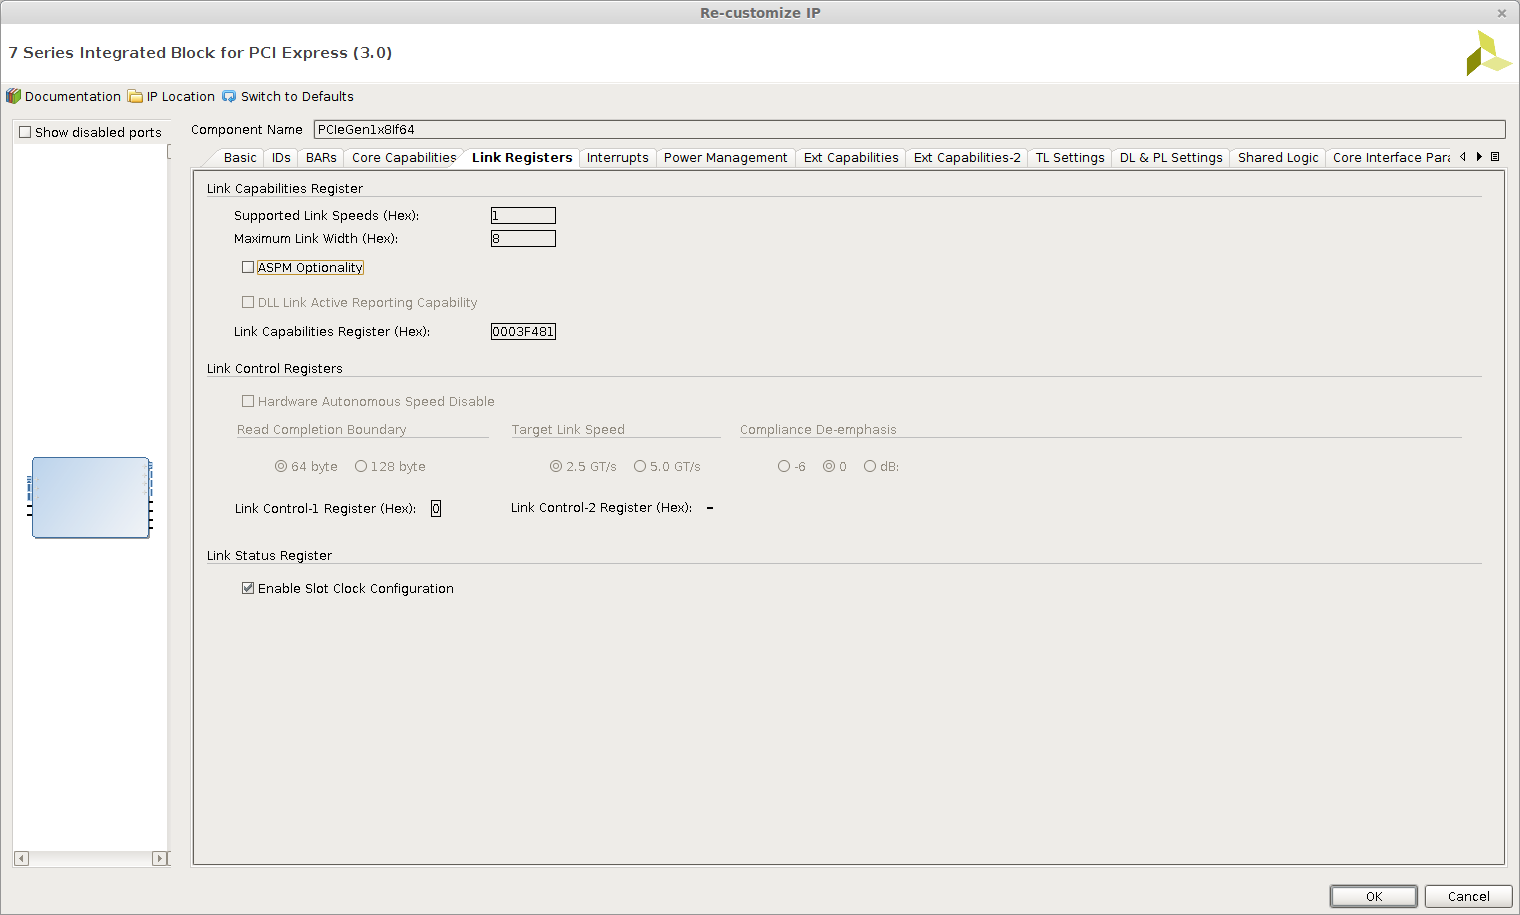
\includegraphics[width=350px,center]{7SeriesIntegratedTabLinkRegisters.png}
%   \label{Fig:7SeriesIntegrated:Generating:7SeriesIntegratedTabLinkRegisters}
% \end{figure}
\begin{figure}[H]
  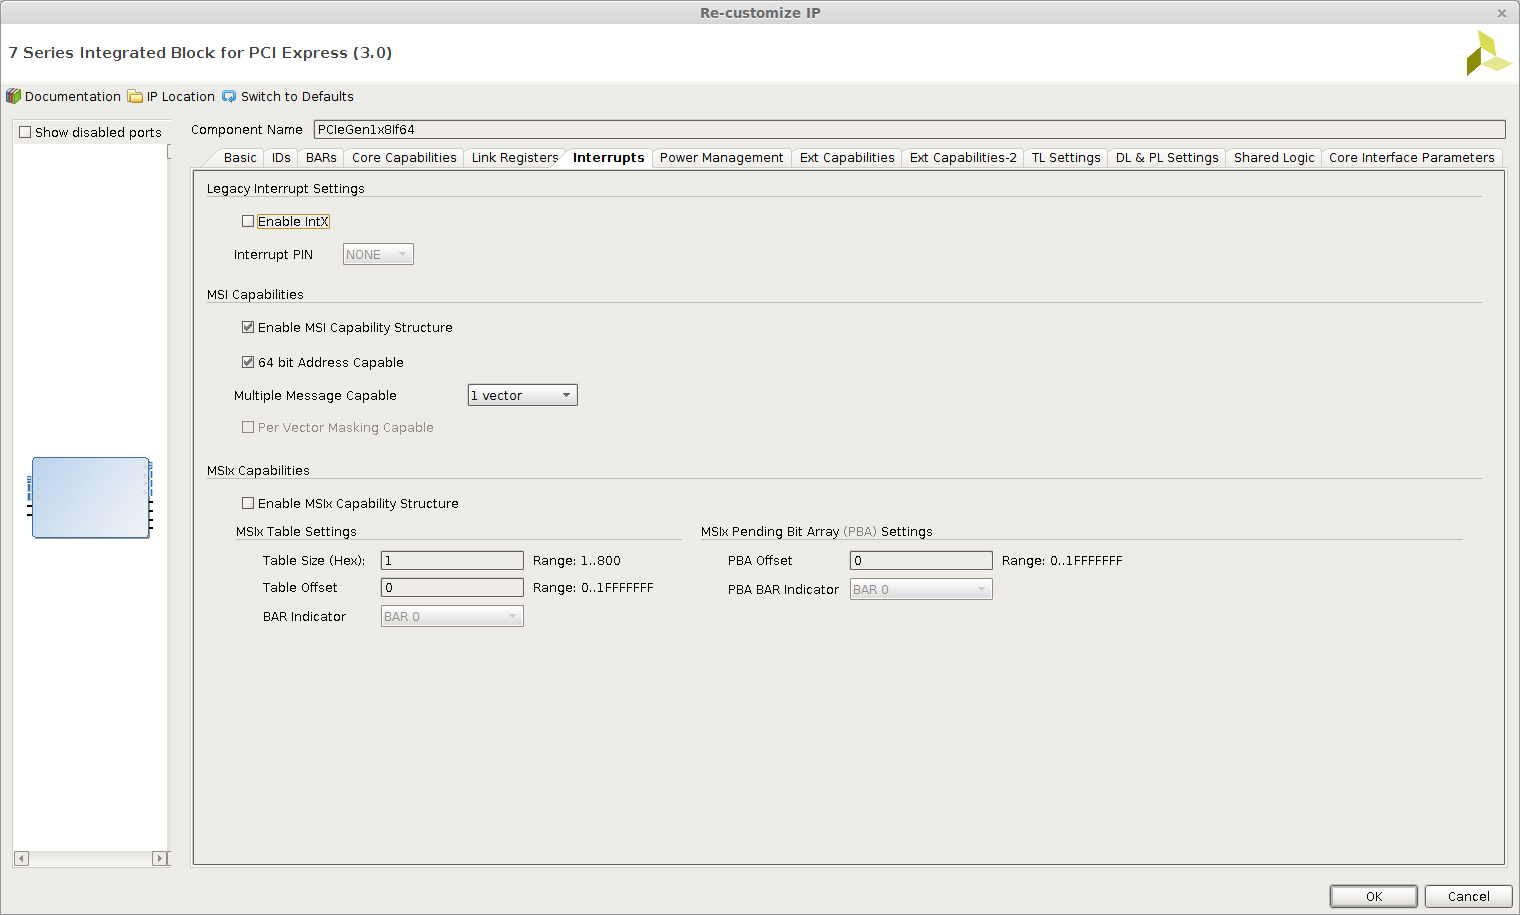
\includegraphics[width=350px,center]{7SeriesIntegratedTabInterrupts.png}
  \caption{PCI Express Interrupts Tab.}
  \label{Fig:7SeriesIntegrated:Generating:7SeriesIntegratedTabInterrupts}
\end{figure}
In the Interrupts Tab shown in
Figure~\ref{Fig:7SeriesIntegrated:Generating:7SeriesIntegratedTabInterrupts}
\ConfigSetting{clear} the checkbox for \ConfigSetting{Enable INTx} (To disable
INTx). The remaining options should match those shown in
Figure~\ref{Fig:7SeriesIntegrated:Generating:7SeriesIntegratedTabInterrupts}
% \begin{figure}[H]
%   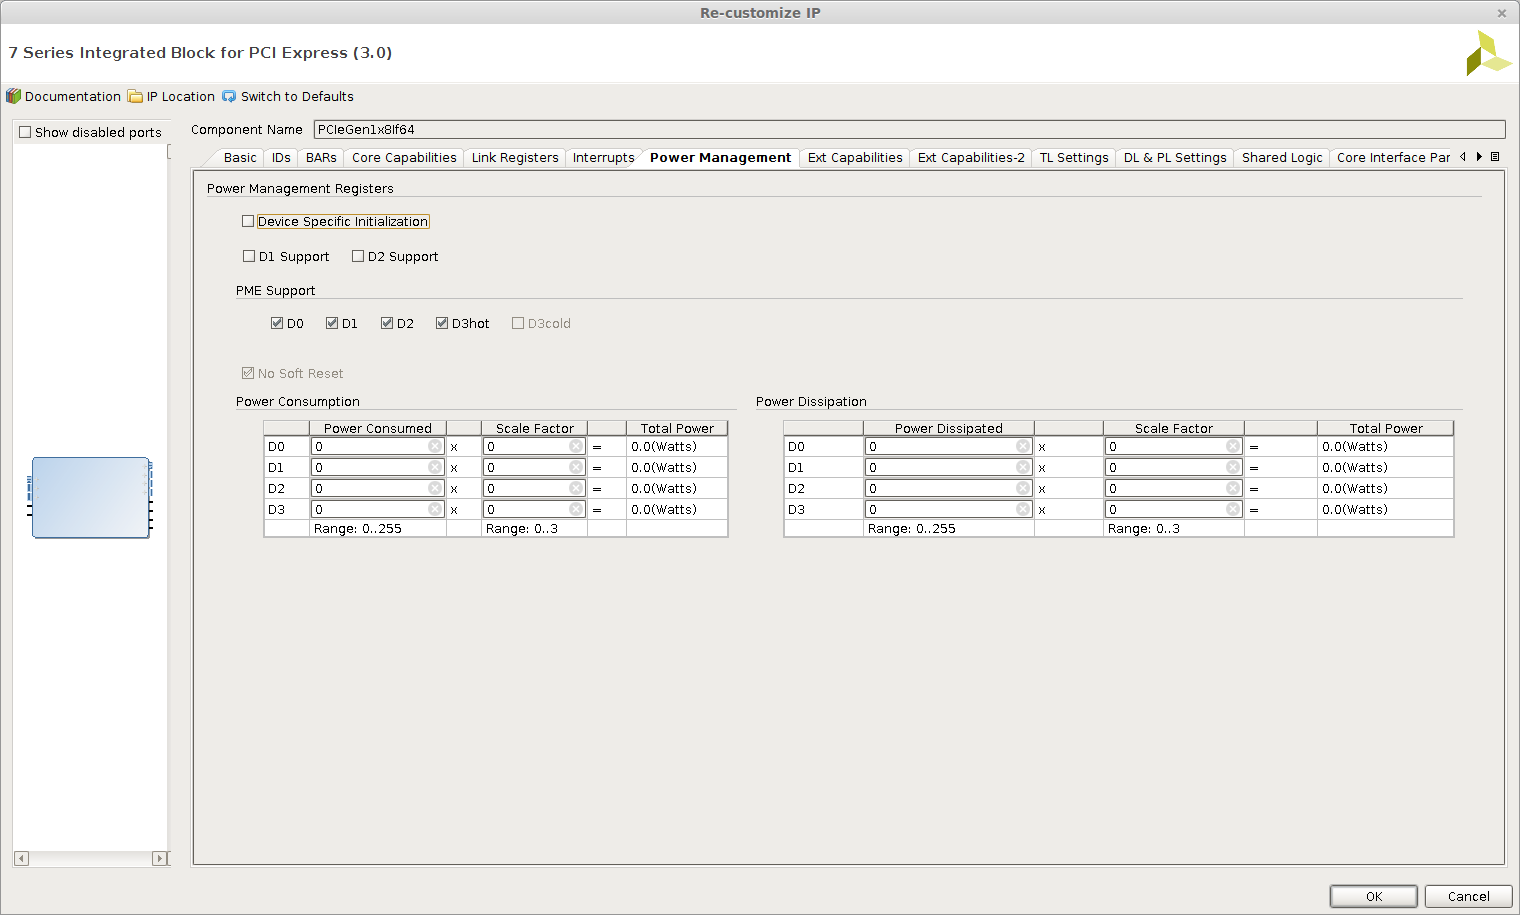
\includegraphics[width=350px,center]{7SeriesIntegratedTabPowerManagement.png}
%   \label{Fig:7SeriesIntegrated:Generating:7SeriesIntegratedTabPowerManagement}
%   \caption{PCI Express Power Manement Tab.}\\ 
% \end{figure}
% \begin{figure}[H]
%   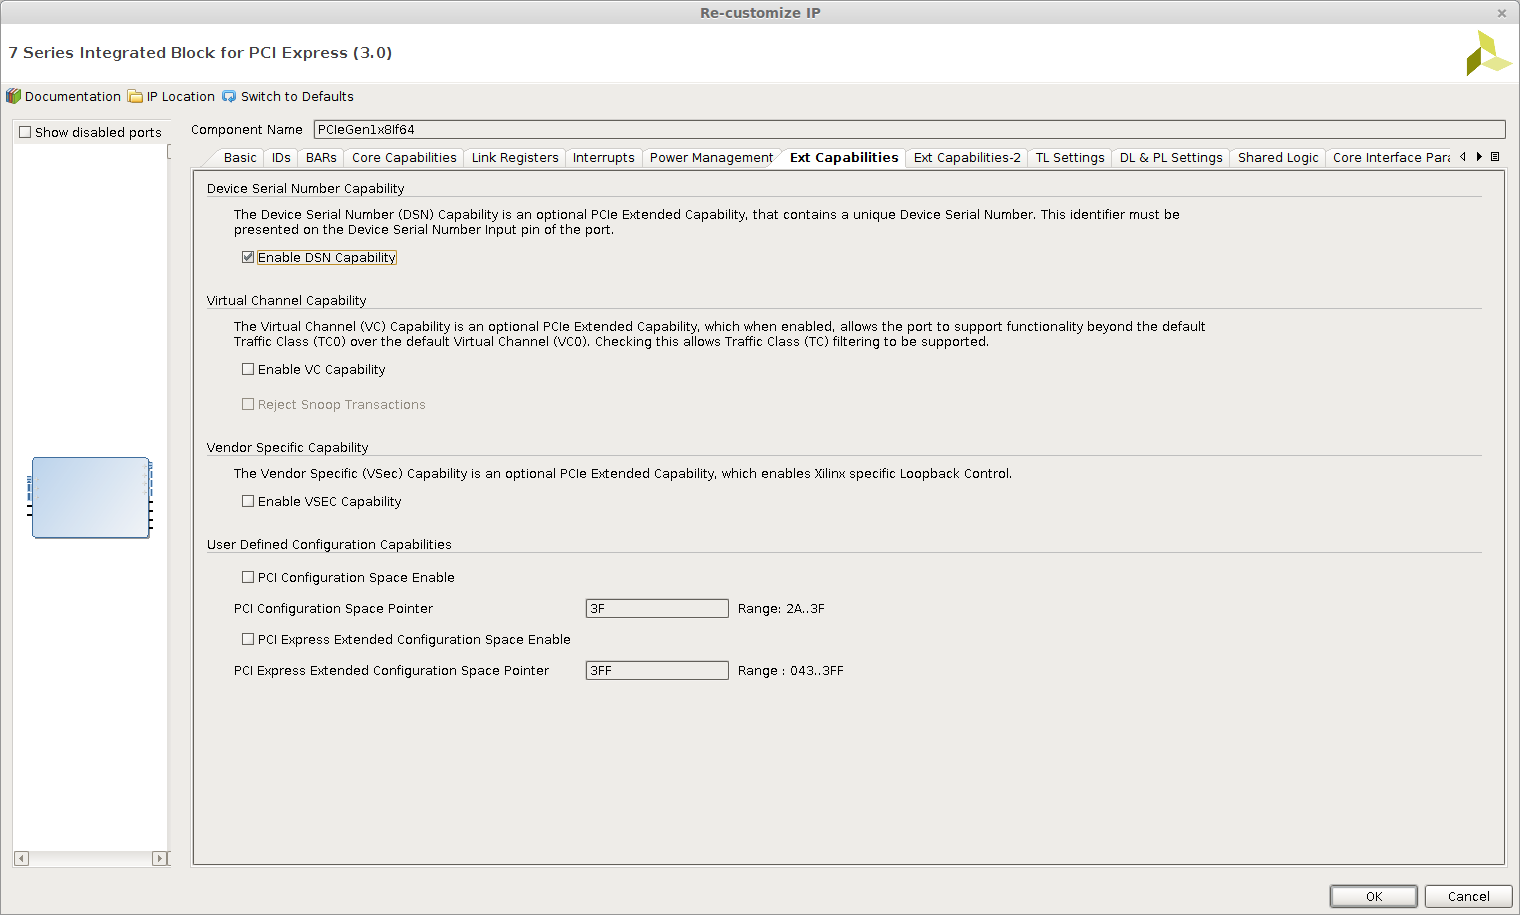
\includegraphics[width=350px,center]{7SeriesIntegratedTabExtCapabilities.png}
%   \label{Fig:7SeriesIntegrated:Generating:7SeriesIntegratedTabExtCapabilities}
% \end{figure}
% \begin{figure}[H]
%   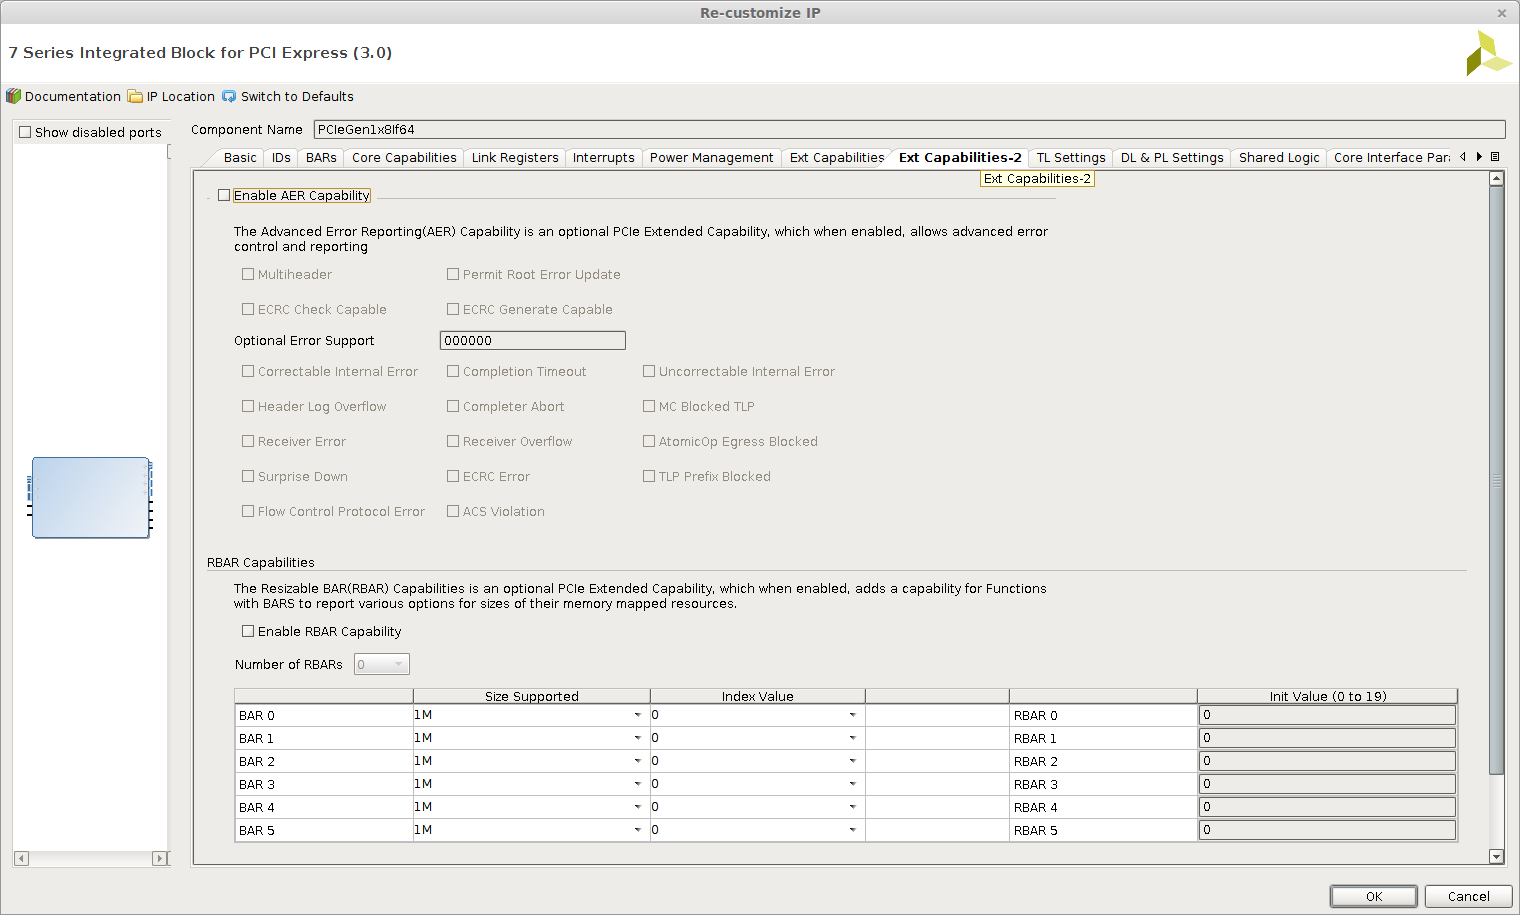
\includegraphics[width=350px,center]{7SeriesIntegratedTabExtCapabilities2.png}
%   \label{Fig:7SeriesIntegrated:Generating:7SeriesIntegratedTabExtCapabilities2}
% \end{figure}
% \begin{figure}[H]
%   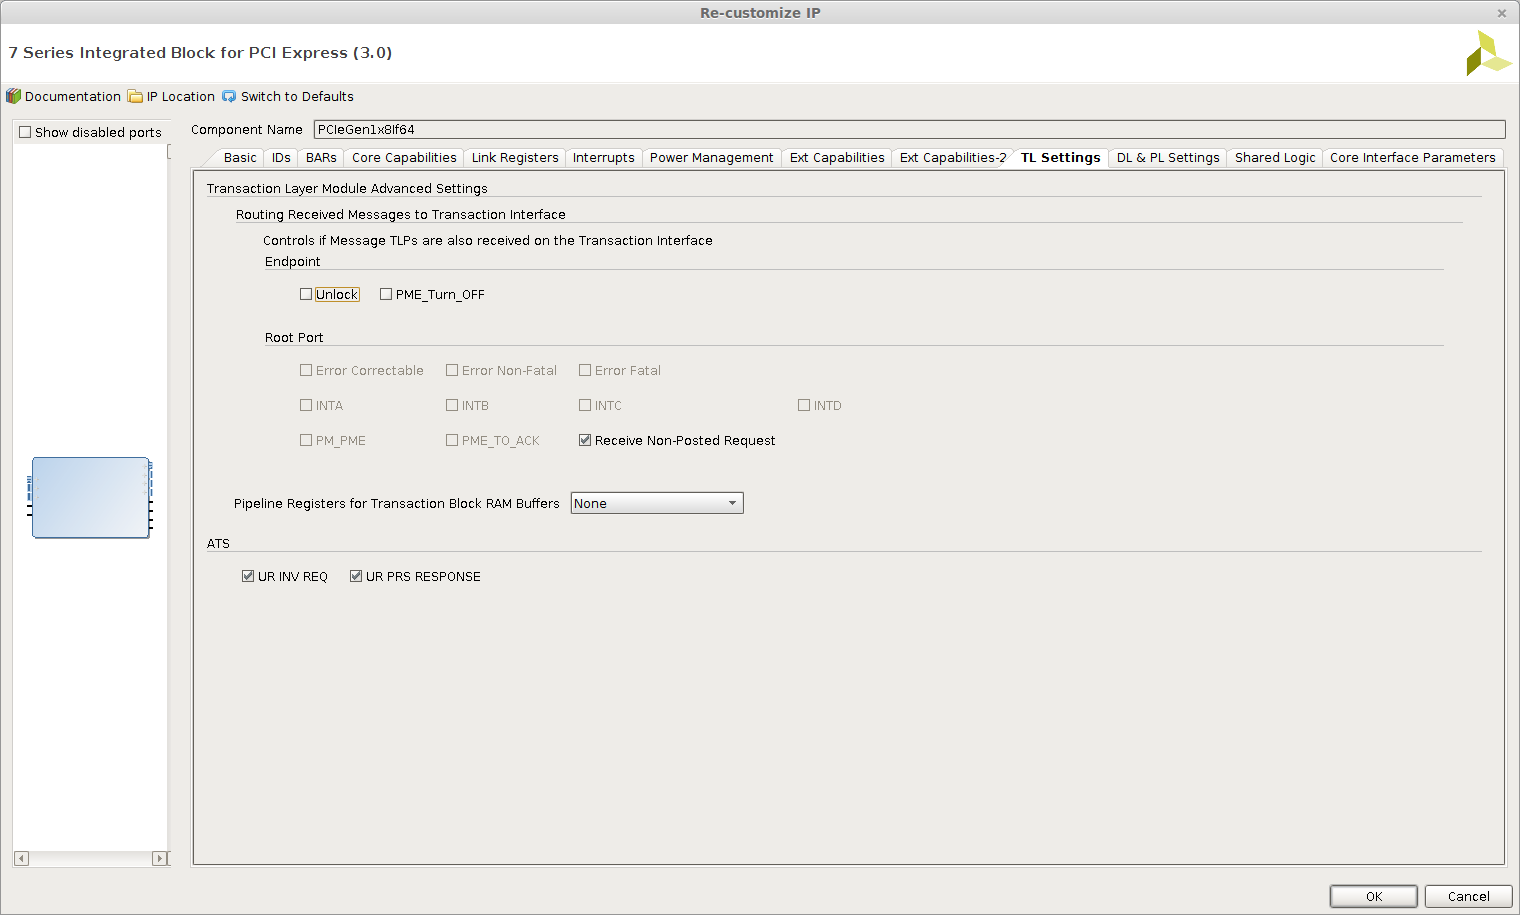
\includegraphics[width=350px,center]{7SeriesIntegratedTabTLSettings.png}
%   \label{Fig:7SeriesIntegrated:Generating:7SeriesIntegratedTabTLSettings}
% \end{figure} 
% \begin{figure}[H]
%   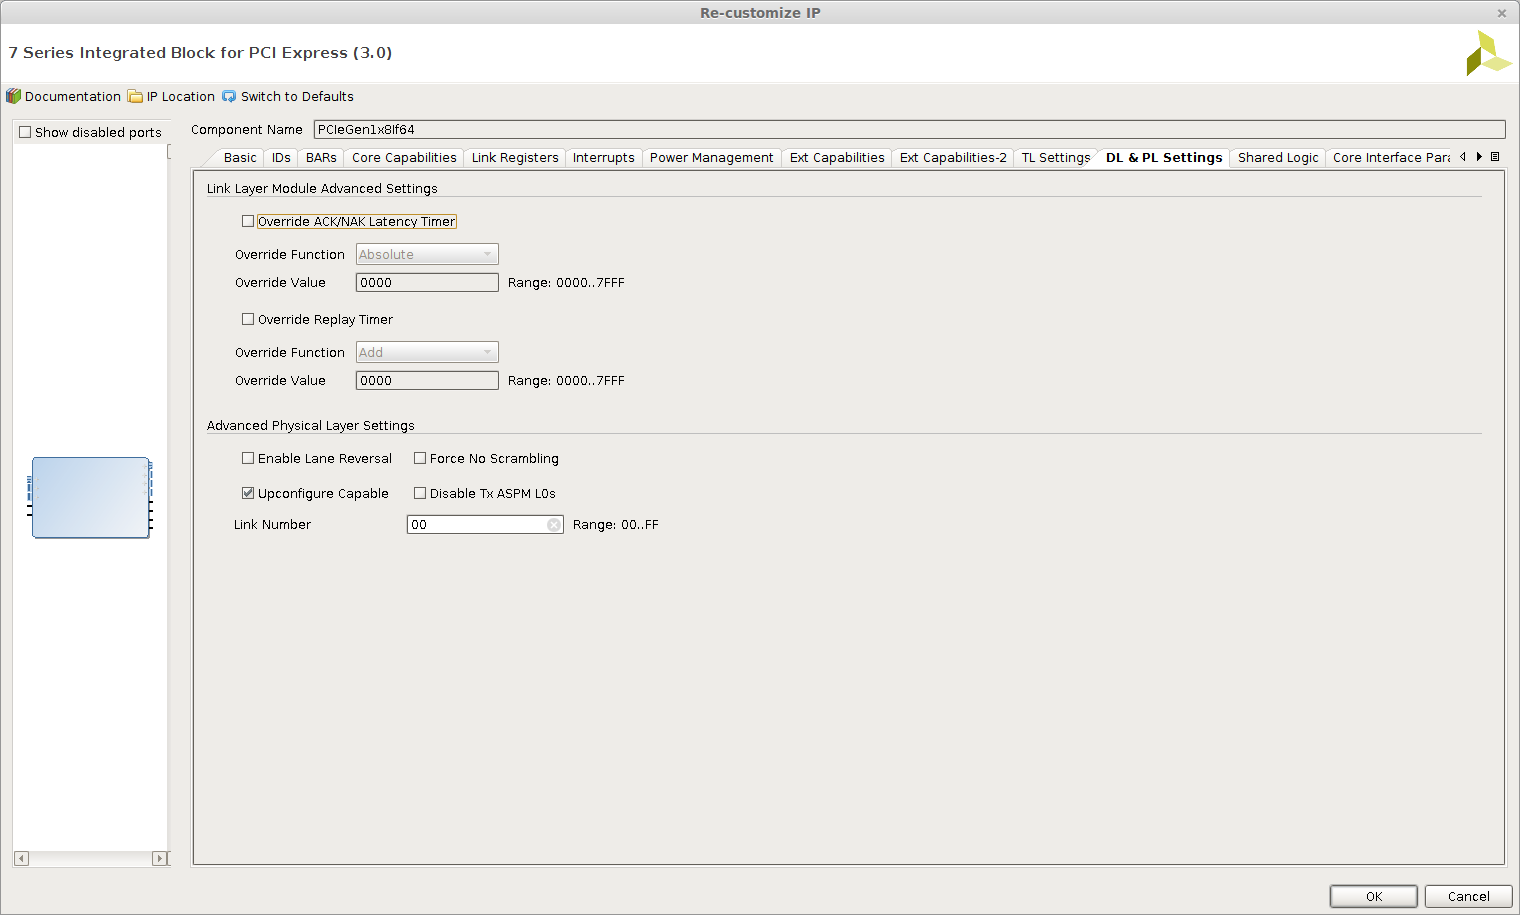
\includegraphics[width=350px,center]{7SeriesIntegratedTabDLPLSettings.png}
%   \label{Fig:7SeriesIntegrated:Generating:7SeriesIntegratedTabDLPLSettings}
% \end{figure}
\begin{figure}[H]
  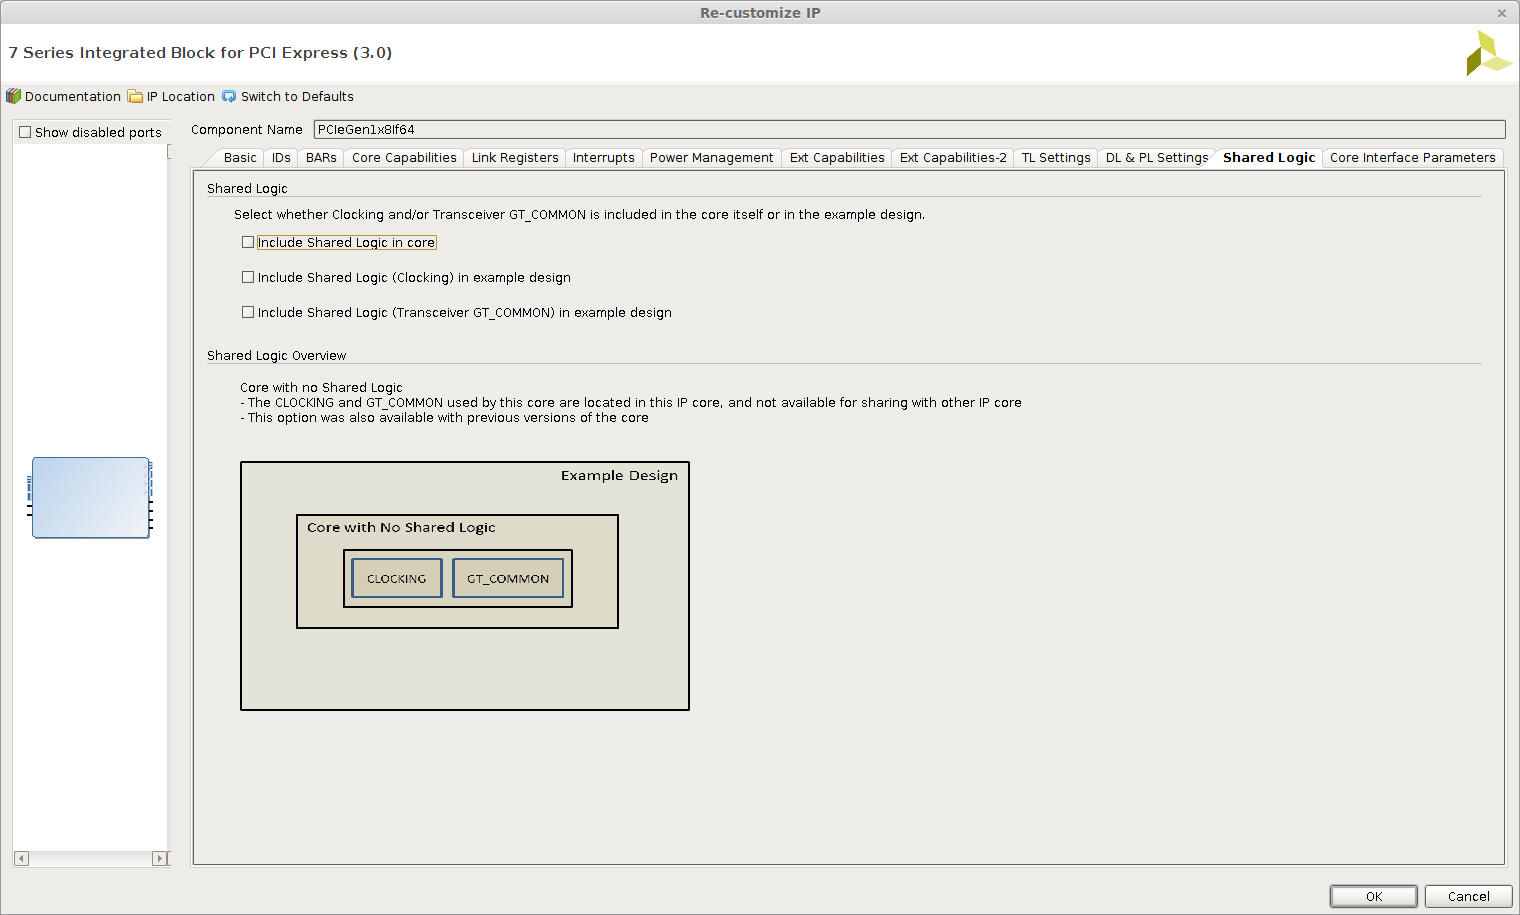
\includegraphics[width=350px,center]{7SeriesIntegratedTabSharedLogic.png}
  \caption{Shared Logic Tab}
  \label{Fig:7SeriesIntegrated:Generating:7SeriesIntegratedTabSharedLogic}
\end{figure}
In the Shared Logic Tab shown in
Figure~\ref{Fig:7SeriesIntegrated:Generating:7SeriesIntegratedTabSharedLogic}
\ConfigSetting{clear} all of the checkboxes shown. These settings will not affect the core
generated, but will affect the example designs generated by Vivado. As a result,
the Example Design will mirror the RIFFA example design provided.
\begin{figure}[H]
  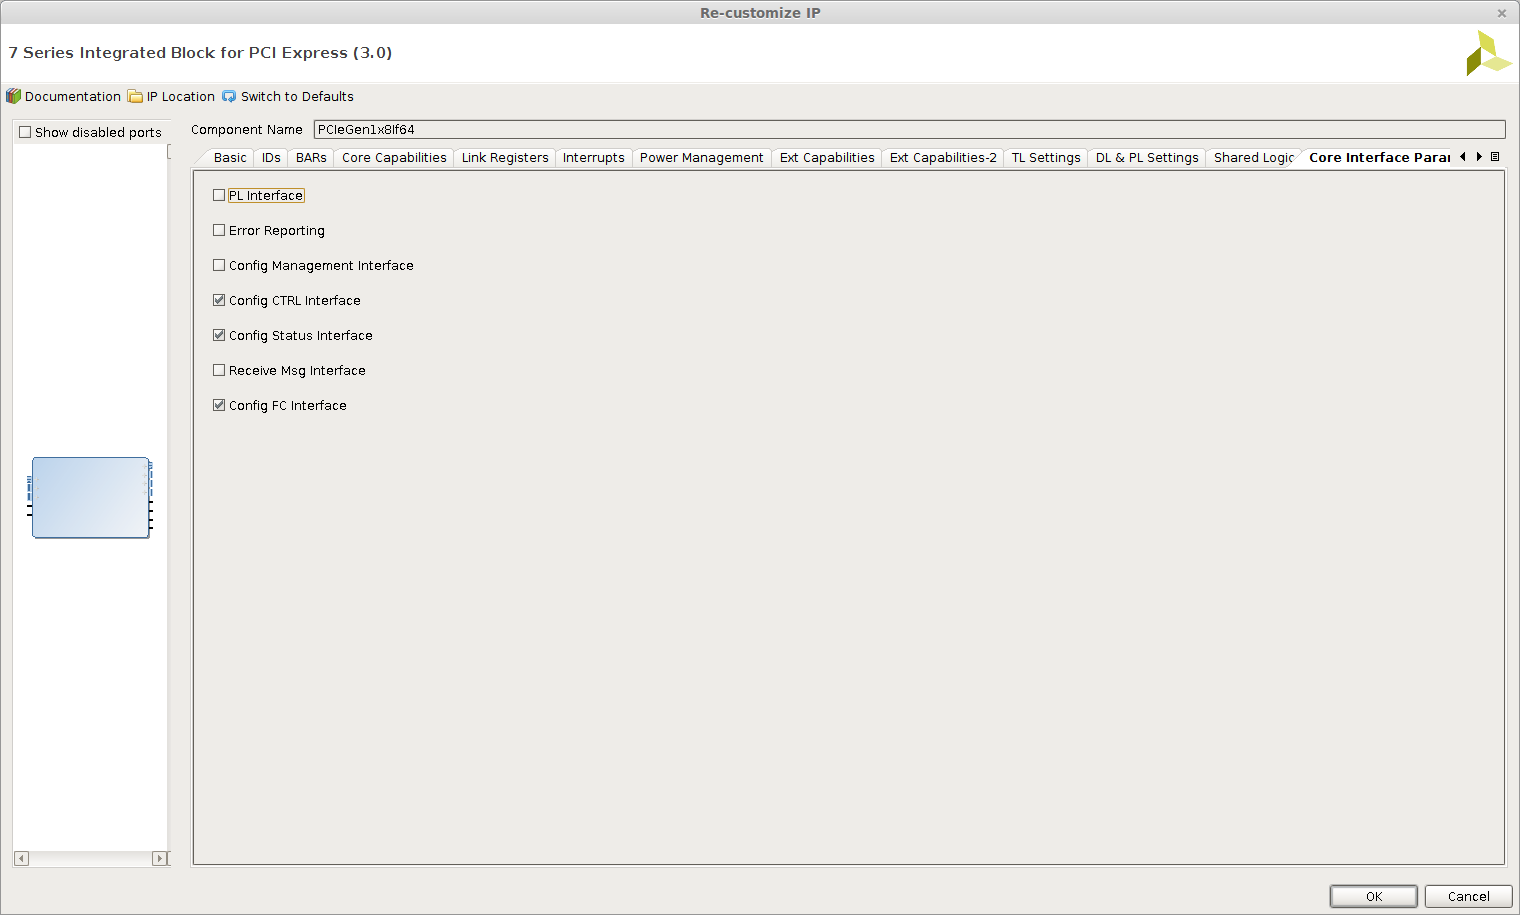
\includegraphics[width=350px,center]{7SeriesIntegratedTabCoreInterfaceParameters.png}
  \caption{Core Interface Parameters Tab}
  \label{Fig:7SeriesIntegrated:Generating:7SeriesIntegratedTabInterfaceParameters}
\end{figure}
Finally, in the Interface Parameters tab, match the checkboxes shown in
Figure~\ref{Fig:7SeriesIntegrated:Generating:7SeriesIntegratedTabInterfaceParameters}. These
options simplify the interface to the generated core

\subsection{Creating Constraints files for the VC707 Development Board}
\label{Sec:7SeriesIntegrated:Generating:Constraints:VC707}
When generating a design for the VC707 board, the following constraints will
correctly constrain the clocks. When using a different board, read the user
guide for appropriate pin placment, or copy the constraints from the PCIe
Endpoint Example Design. The remaining constraints are contained the generated PCIe IP.
\begin{lstlisting}[basicstyle=\footnotesize\ttfamily,language=tcl,
    commentstyle=\color{red},label=Listing:7SeriesIntegrated:Generating:Constraints:VC707,
    caption=\Xilinx{.xdc} constraints for the VC707 board,frame=single]
  set_property PACKAGE_PIN AV35 [get_ports PCIE_RESET_N]
  set_property IOSTANDARD LVCMOS18 [get_ports PCIE_RESET_N]
  set_property PULLUP true [get_ports PCIE_RESET_N]
  # The following constraints are BOARD SPECIFIC. This is for the VC707
  set_property LOC IBUFDS_GTE2_X1Y5 [get_cells refclk_ibuf]
  create_clock -period 10.000 -name pcie_refclk [get_pins refclk_ibuf/O]
  set_false_path -from [get_ports PCIE_RESET_N]
\end{lstlisting}

\subsection{Creating Constraints files for the ZC706 Development Board}
\label{Sec:7SeriesIntegrated:Generating:Constraints:ZC706}
When generating a design for the ZC706 board, the following constraints will
correctly constrain the clocks. When using a different board, read the user
guide for appropriate pin placment, or copy the constraints from the PCIe
Endpoint Example Design. The remaining constraints are contained the generated PCIe IP.
\begin{lstlisting}[basicstyle=\footnotesize\ttfamily,language=tcl,
    commentstyle=\color{red},label=Listing:7SeriesIntegrated:Generating:Constraints:ZC706,
    caption=\Xilinx{.xdc} constraints for the ZC706 board,frame=single]
  set_property IOSTANDARD LVCMOS15 [get_ports PCIE_RESET_N]
  set_property PACKAGE_PIN AK23 [get_ports PCIE_RESET_N]
  set_property PULLUP true [get_ports PCIE_RESET_N]
  # The following constraints are BOARD SPECIFIC. This is for the ZC706
  set_property LOC IBUFDS_GTE2_X0Y6 [get_cells refclk_ibuf]
  create_clock -period 10.000 -name pcie_refclk [get_pins refclk_ibuf/O]
  set_false_path -from [get_ports PCIE_RESET_N]
\end{lstlisting}


\pagebreak
\section{Ultrascale - Gen3 Integrated Block for PCI Express - (VC709 and newer)}
This is a step by step guide for building a RIFFA \RIFFAVer~reference design for
Xilinx FPGA's compatible with the Gen3 Integrated Block for PCI Express. In
RIFFA \RIFFAVer~there are three example designs for the VC709 board in the
\Directory{RIFFA \RIFFAVer/source/fpga/vc709} directory:
\VCSevenOhNineExampleDesignsLong. To use one of these example designs, follow
the instructions below.

\subsection{VC709 Example Designs}
\label{Sec:Gen3Integrated:ExampleDesign}
\begin{enumerate}
\item Open Vivado to get the introductory screen shown in
  Figure~\ref{Fig:Vivado:WelcomeScreen}.
\item Click 'Open an Existing Project' and navigate to your RIFFA
  \RIFFAVer~directory.
\item In the RIFFA \RIFFAVer~distribution, open \Directory{RIFFA
  \RIFFAVer/source/fpga/xilinx/vc709/} and choose from one of the existing
  example design directories for your board. In the example design directory,
  locate the \Directory{prj} folder and open it. Select the .xpr file and click
  open. This will open the example project, as shown in
  Figure~\ref{Fig:Gen3Integrated:ExampleDesign:ProjectOpened}.
\item This project was compiled in Vivado \VivadoVer. The bit file generated can
  be used to test the FPGA system. If you are using a newer version of Vivado,
  recompile the example design or use the programming file provided.
  \begin{itemize}
  \item IP Settings are now packaged as part of the example designs! Users no
    longer need to generate IP.
  \item To recompile the example design, click the generate bitstream button in
    the top left corner as shown in
    Figure~\ref{Fig:Gen3Integrated:ExampleDesign:ProjectOpened}.
  \item Recompiling your design will generate a new bitfile in the Xilinx
    project. The bit file in the \Directory{bit} will not be changed.
  \end{itemize}
\item To program the FPGA, click 'Open Hardware Manager'. New bit files
  (generated by Vivado) will appear in the Vivado generated directories. An
  example bit file is provided in the example design's \Directory{bit}. Load the
  bitstream to your VC709 board and restart your computer.
  \begin{itemize}
  \item Before programming your FPGA, you should install the RIFFA driver. See
    Section~\ref{Sec:RIFFA:Installation}
  \end{itemize}
\item The example design uses the chnl\_tester (shown in
  Figure~\ref{Fig:Vivado:ExampleDesign:chnl_tester}, which works with
  the example software in the \Directory{source/\{C\_C++,Java,python,matlab\}}
  directories. Replace the chnl\_tester instantiation with any user logic,
  matching the RIFFA interface.
\item Recompile the design and program the FPGA Device. Changing the
  \RIFFAParameter{C\_NUM\_CHNL} will change the number of independent channel
  interfaces
\end{enumerate}
\begin{figure}
  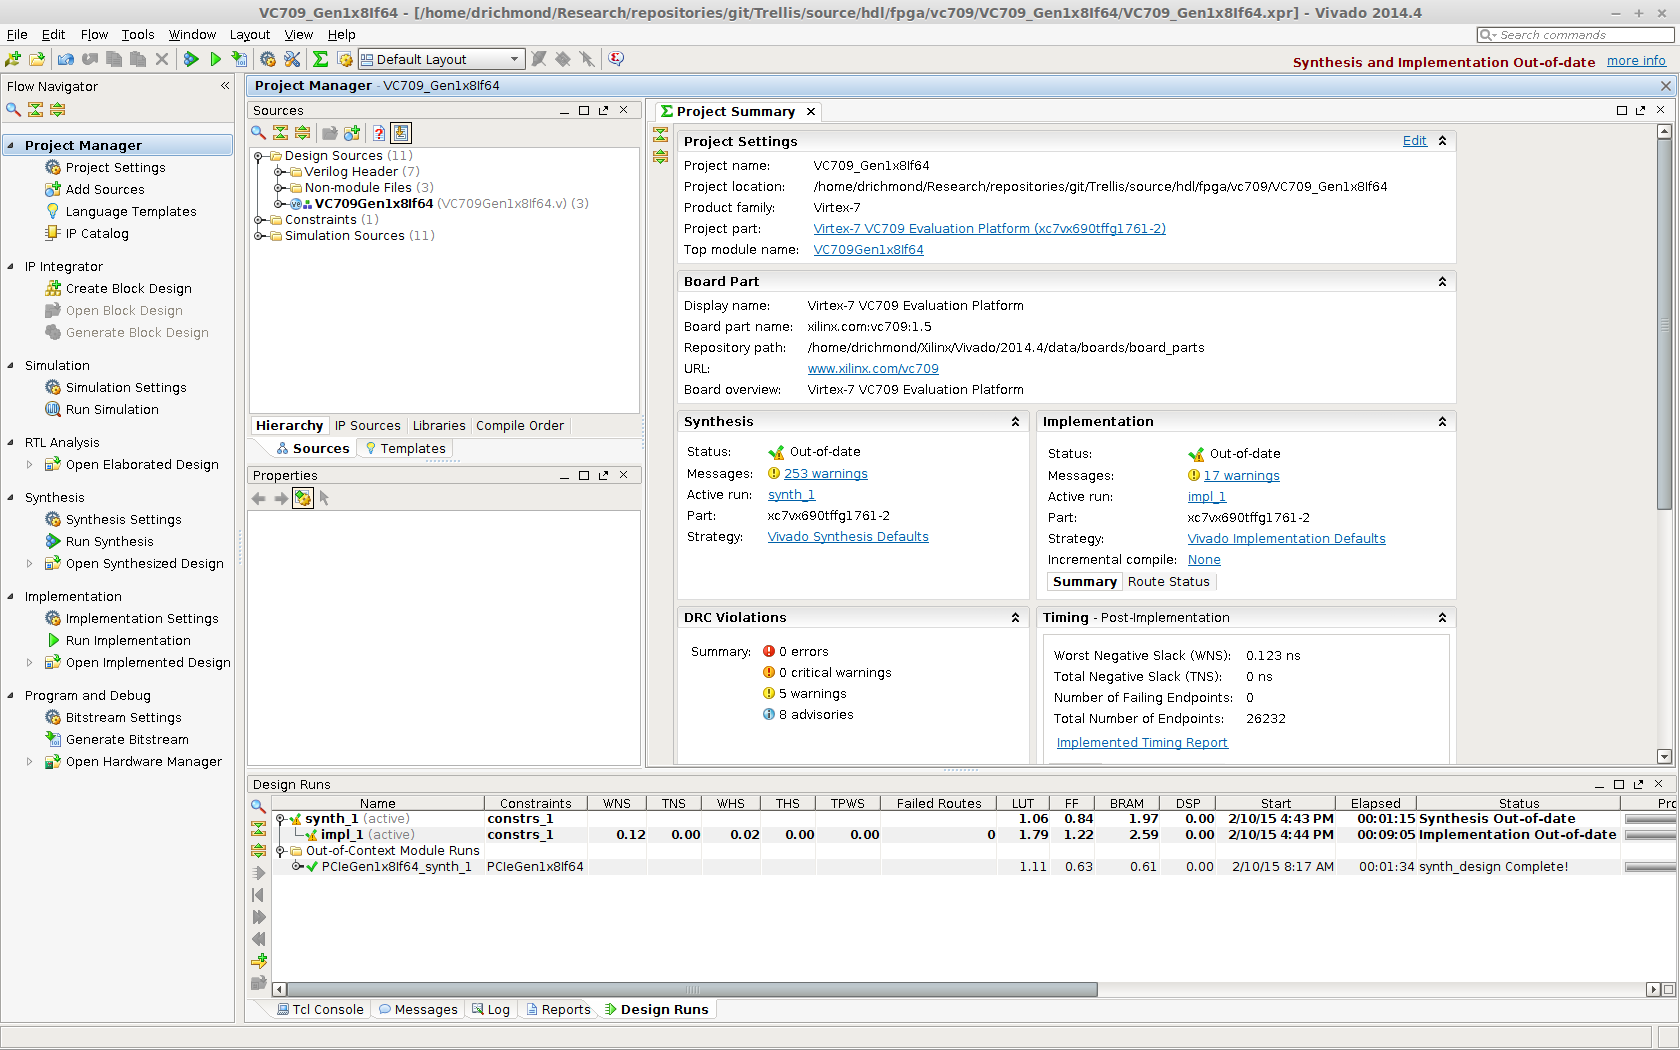
\includegraphics[width=300px,center]{Gen3IntegratedOpenProject.png}
  \caption{Project Splash Screen for Gen3 Integrated Block for PCI Express Projects}
  \label{Fig:Gen3Integrated:ExampleDesign:ProjectOpened}
\end{figure}
\subsection{Generating the Gen3 Integrated Block for PCI Express}
\label{Sec:Gen3Integrated:Generating}
The following steps are not required for general users. See the instructions
above for how to compile RIFFA.

Alternatively, it is possible to generate the PCIe Endpoint with different
settings than those provided in the example design. Changing the endpoint
settings is required when changing the parameters
\RIFFAParameter{C\_PCI\_DATA\_WIDTH}, \RIFFAParameter{C\_MAX\_PAYLOAD\_BYTES}
and \RIFFAParameter{C\_LOG\_NUM\_TAGS}. The \RIFFAParameter{C\_NUM\_LANES} is a
parameter in the top level file of each example project. How these parameters
relate to IP core settings is highlighted in the following figures.

If the goal is to generate a RIFFA design completely from scratch, each board
directory comes with a RIFFA wrapper verilog file and instantiates a
vendor-specific translation layer. It is highly recommended to re-use these
files RIFFA wrapper when creating designs from scratch.

To generate the PCIe IP select the 7 Series Integrated Block for PCI Express
after selecting the IP Catalog shown in
Figure~\ref{Fig:Gen3Integrated:ExampleDesign:ProjectOpened}. This will open the
IP Customization window as shown in
Figure~\ref{Fig:Gen3Integrated:Generating:Gen3IntegratedTabBasic}

\begin{figure}[H]
  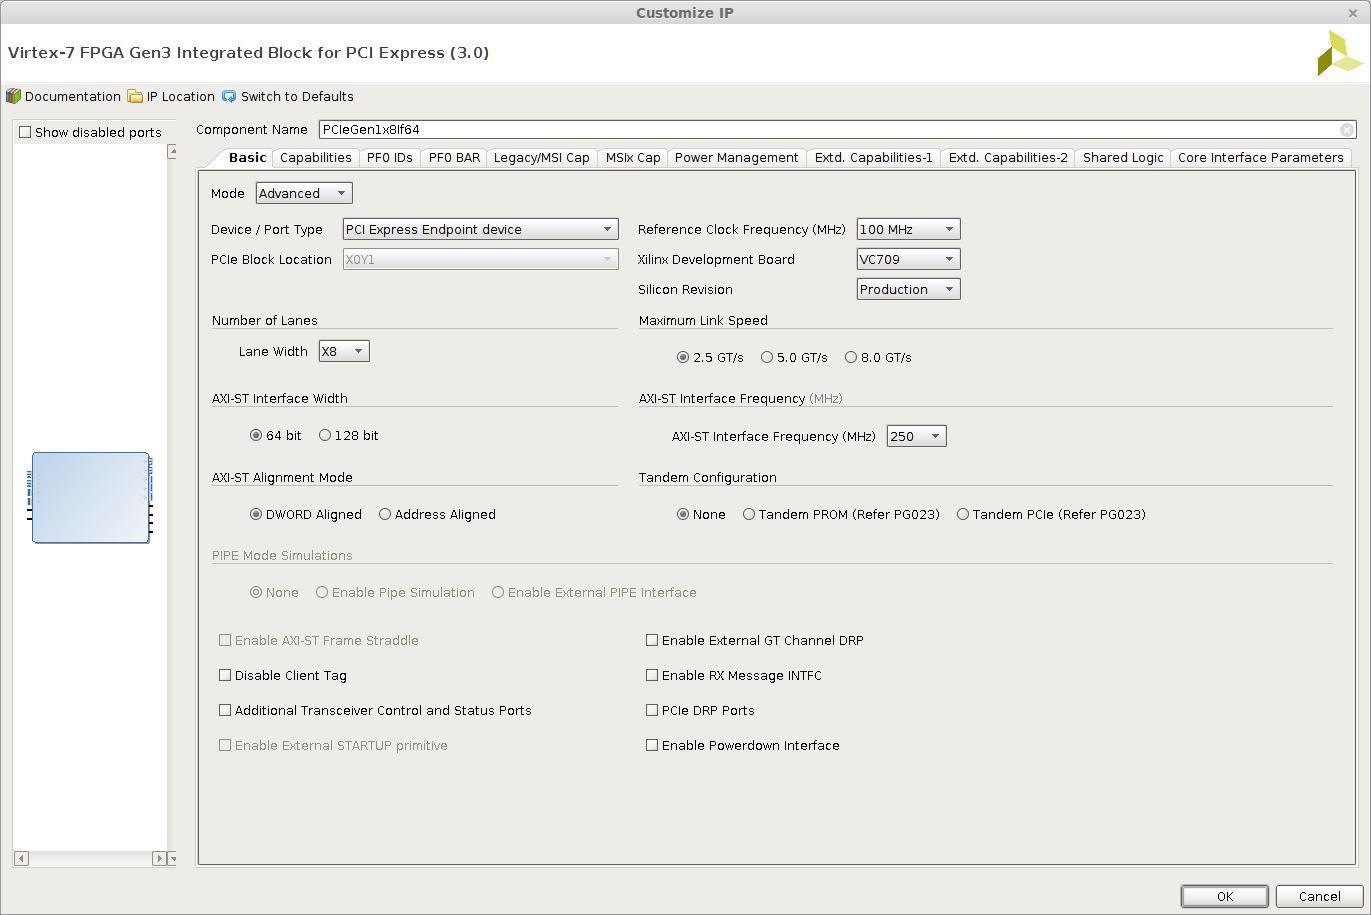
\includegraphics[width=\figurewidth,center]{Gen3IntegratedTabBasic.png}
  \caption{Basic settings tab.}
  \label{Fig:Gen3Integrated:Generating:Gen3IntegratedTabBasic}
\end{figure}
First, select ``ADVANCED'' from the drop down menu. This will cause more tabs to
appear in the bar. The following tabs are not used during customization: MSIx Cap (Capabilities),
Extd. Capabilities 1, and Extd Capabilites 2.

In this example, we have set the \ConfigSetting{Xilinx Development Board} to
\ConfigSetting{VC709}, and selected the PCIe Gen1 rate of \ConfigSetting{2.5
  GT/s}, and a Lane Width of 8 (\RIFFAParameter{C\_NUM\_LANES} = 8). We have
chosen to set the \ConfigSetting{AXI Interface Width} to \ConfigSetting{64-bits}
(\RIFFAParameter{C\_PCI\_DATA\_WIDTH} = 64). Finally Clear the
\ConfigSetting{Disable Client Tag} and \ConfigSetting{PCIe DRP Ports} boxes. The
choice of \ConfigSetting{Link Rate}, \ConfigSetting{Lanes}, and
\ConfigSetting{Interface Width} will allow different AXI Interface Frequencies
to be selected. The RIFFA core will run at this clock frequency, but the user
logic can run at whatever frequency it desires.

Optional: Set the Component Name of the PCI Express block, and the IP
Location. In our example projects, we use the name template
PCIeGen\textbf{W}x\textbf{Y}If\textbf{Z} where \textbf{W} is the PCI Express
Version (\ConfigSetting{Link Speed} in
Figure~\ref{Fig:Gen3Integrated:Generating:Gen3IntegratedTabBasic}),
\textbf{Y} is the lane width, and \textbf{Z} is the AXI interface width.  The IP
location is the \Directory{ip} directory in the example project.

Note: For RIFFA \RIFFAVer~the 256-bit interface is not supported, however the
128-bit interface is. This means PCIe Gen2 with 8 lanes, and PCIe Gen3 with 4
lanes are both supported.

\begin{figure}[H]
  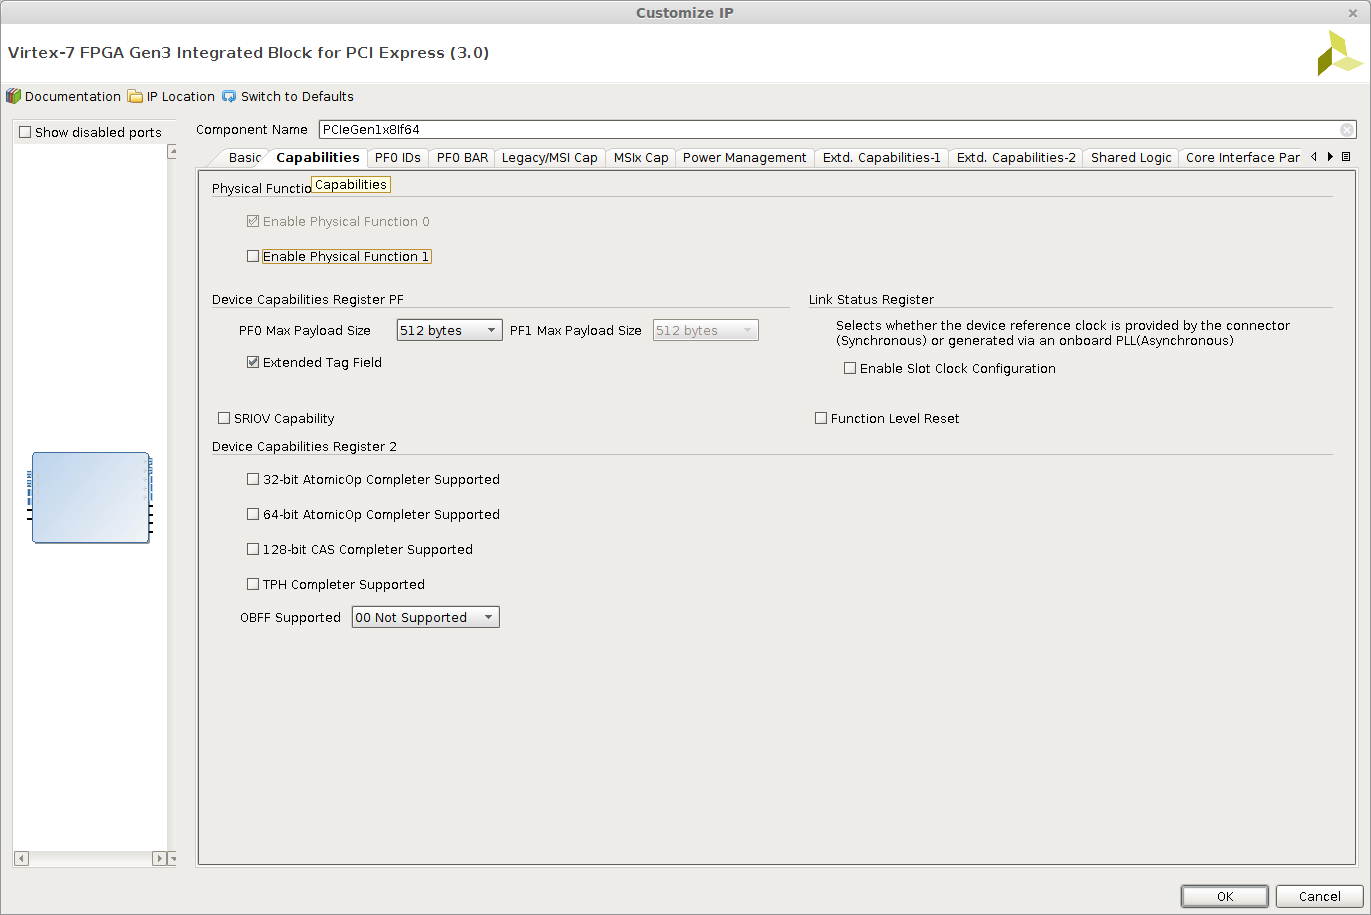
\includegraphics[width=350px,center]{Gen3IntegratedTabCapabilities.png}
  \caption{PCI Express Capabilities Tab.}
  \label{Fig:Gen3Integrated:Generating:Gen3IntegratedTabCapabilities}
\end{figure}
In the Capabilities tab shown in
Figure~\ref{Fig:Gen3Integrated:Generating:Gen3IntegratedTabCapabilities} check
the \ConfigSetting{Extended Tag Field} box. If the \ConfigSetting{Extended Tag
  Field} is selected \RIFFAParameter{C\_LOG\_NUM\_TAGS} = 8, otherwise
\RIFFAParameter{C\_LOG\_NUM\_TAGS} = 5. Set the \ConfigSetting{PFO Max Payload
  Size} from the dropdown menu; Use this to set the RIFFA
\RIFFAParameter{C\_MAX\_PAYLOAD\_BYTES} parameter.

Note: Maximum Payload sizes are typically set by the BIOS, and 256 bytes seems
to be standard. RIFFA will default to the minimum of
\RIFFAParameter{C\_MAX\_PAYLOAD\_SIZE} and the setting in your BIOS. Unless your
BIOS is modified, or can support substantially larger packets, there will be no
performance benefit to increasing the payload size. Increasing the maximum
payload size will increase the resources consumed.

\begin{figure}[H]
  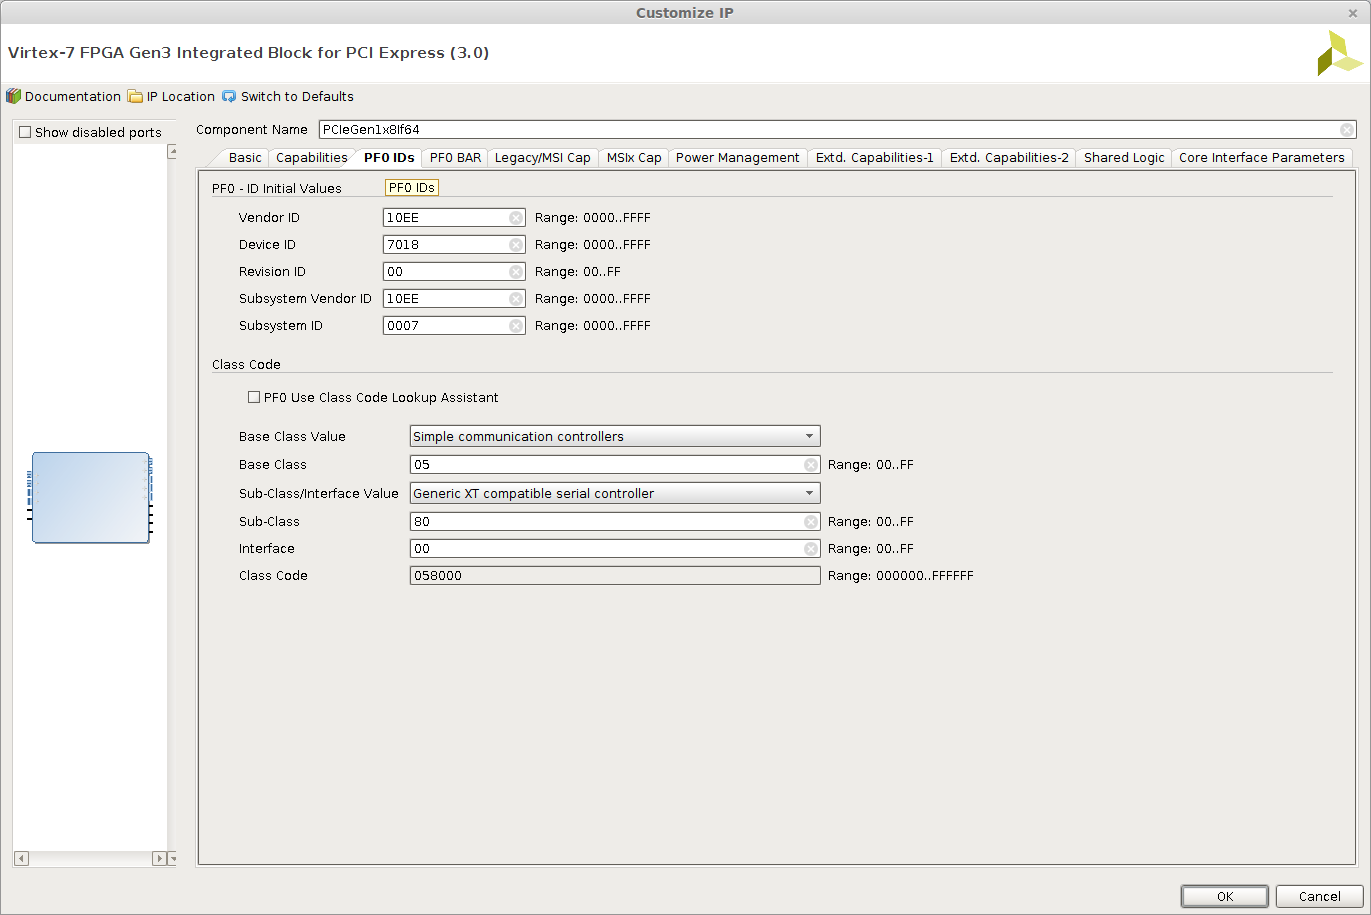
\includegraphics[width=350px,center]{Gen3IntegratedTabPF0Ids.png}
  \caption{PCI Express IDs Tab.}
  \label{Fig:Gen3Integrated:Generating:Gen3IntegratedTabPF0Ids}
\end{figure}
The tab in Figure~\ref{Fig:Gen3Integrated:Generating:Gen3IntegratedTabPF0Ids}
is optional. Setting the Device ID may assist in identifying different FPGAs in
a multi-FPGA system. The other options, specifically the Vendor ID, must remain
the same.
\begin{figure}[H]
  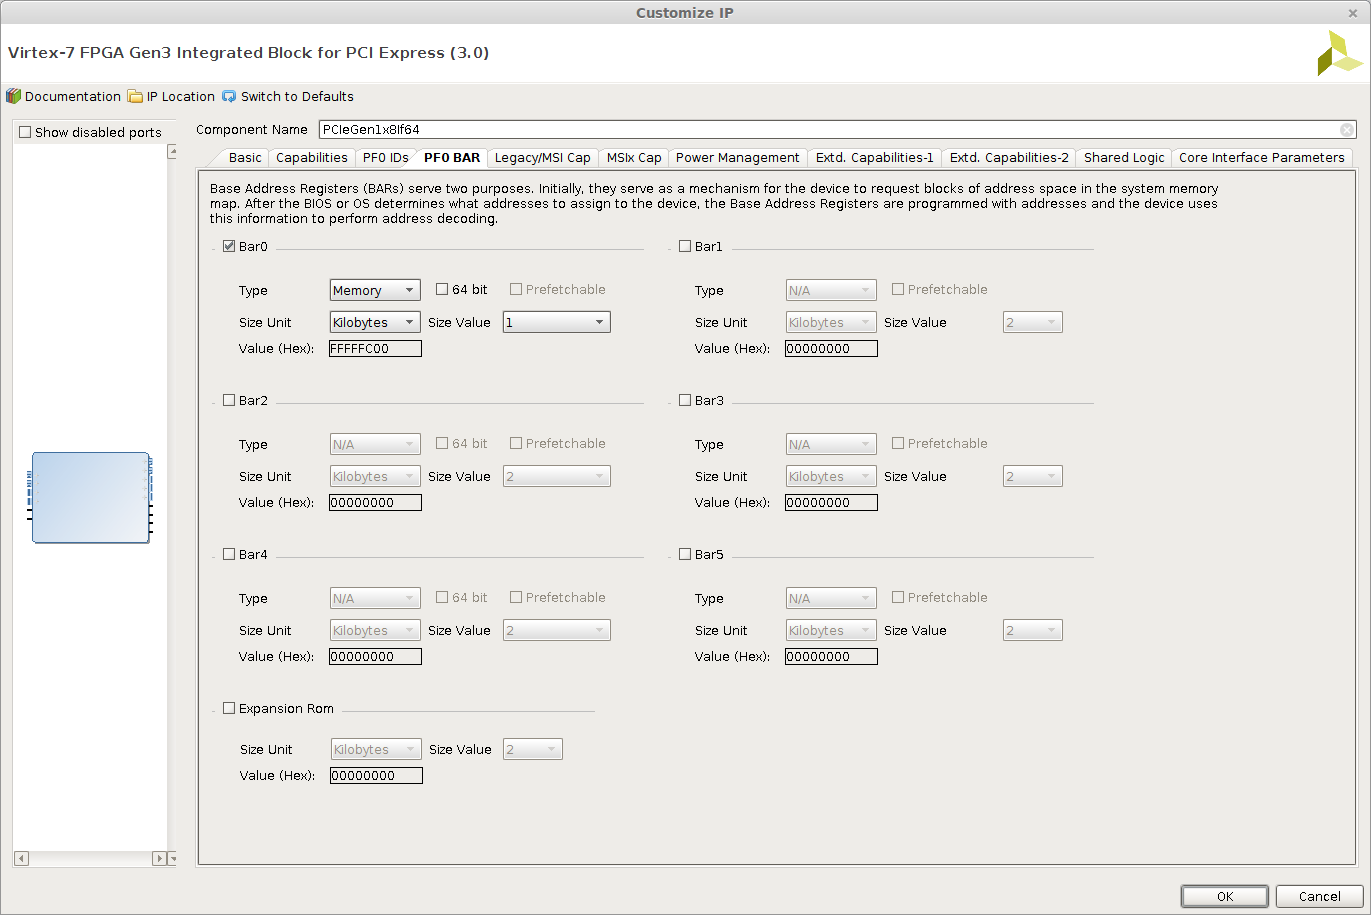
\includegraphics[width=350px,center]{Gen3IntegratedTabPF0Bar.png}
  \caption{PCI Express Base Address Registers (BAR) Tab.}
  \label{Fig:Gen3Integrated:Generating:Gen3IntegratedTabPF0Bar}
\end{figure}
The tab in Figure~\ref{Fig:Gen3Integrated:Generating:Gen3IntegratedTabPF0Bar}
must be configured so that BAR0 is \ConfigSetting{enabled}. Select type
\ConfigSetting{Memory}, and Unit \ConfigSetting{Kilobyte}, and
\ConfigSetting{Size Value} \ConfigSetting{1} from the dropdown menus. If these
values are not set correctly the RIFFA driver will not recognize the FPGA
device.
\begin{figure}[H]
  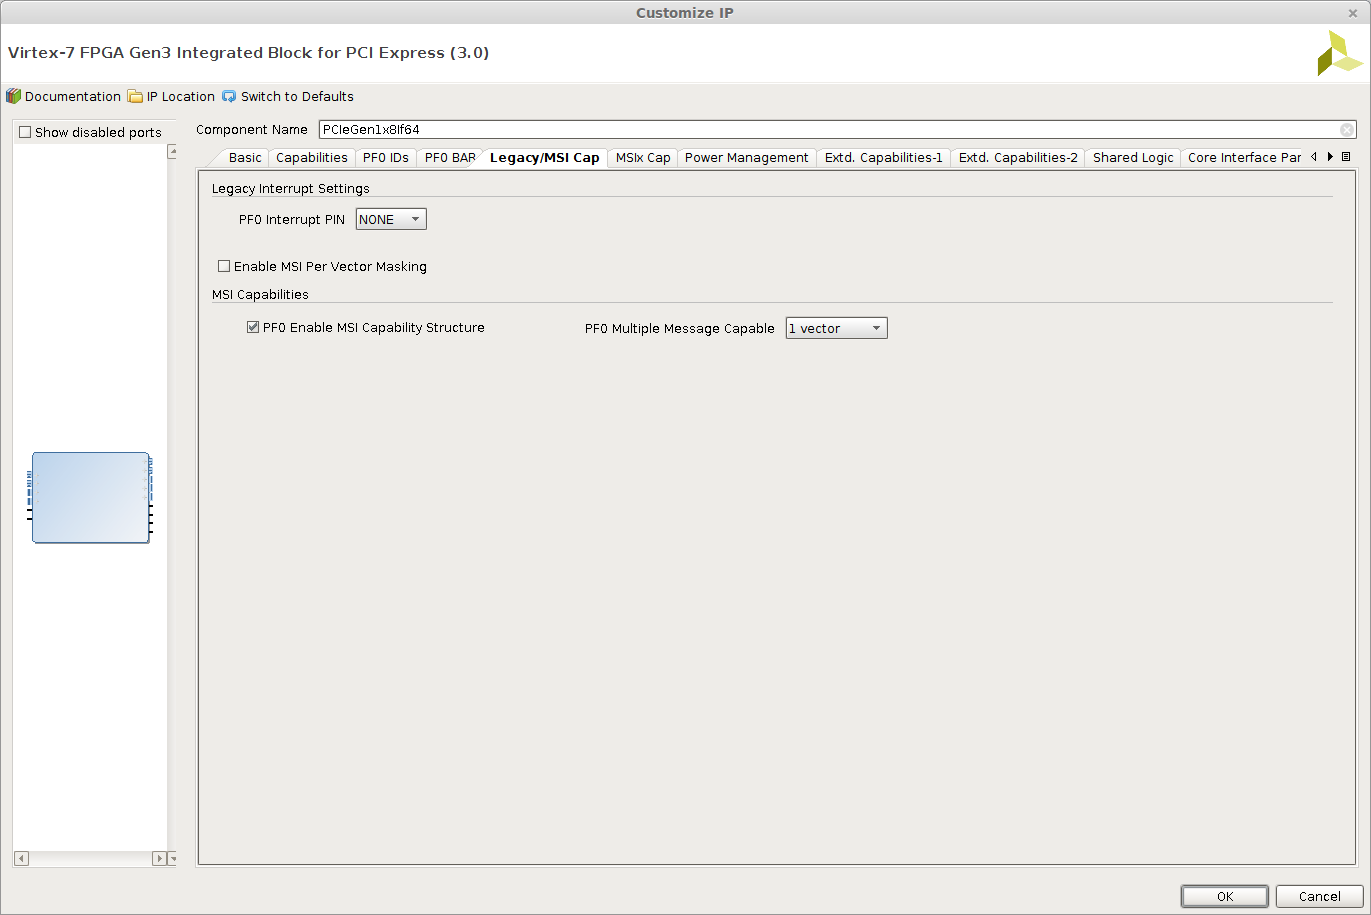
\includegraphics[width=350px,center]{Gen3IntegratedTabLegacyMSICap.png}
  \caption{PCI Express Legacy and MSI Interrupts Tab.}
  \label{Fig:Gen3Integrated:Generating:Gen3IntegratedTabLegacyMSICap}
\end{figure}
In the Legacy/MSI Capabilites tab shown in
Figure~\ref{Fig:Gen3Integrated:Generating:Gen3IntegratedTabLegacyMSICap}, select
\ConfigSetting{None} in the \ConfigSetting{PFO Interrupt Pin Dropdown} menu and
set the \ConfigSetting{PFO Multiple Message Capable} dropdown menu to
\ConfigSetting{1 Vector}
% \begin{figure}[H]
%   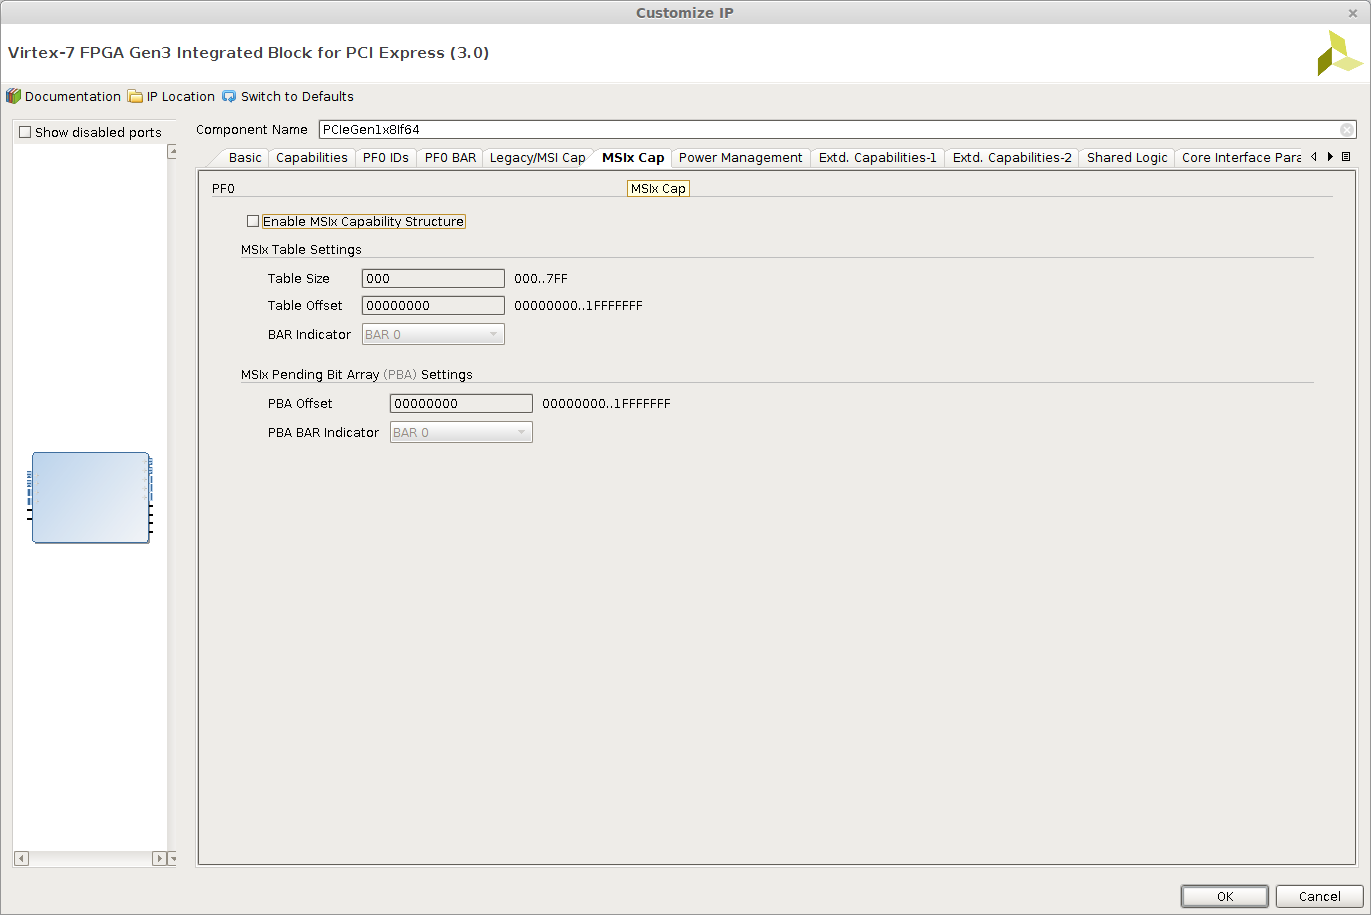
\includegraphics[width=350px,center]{Gen3IntegratedTabMSIxCap.png}
%   \label{Fig:Gen3Integrated:Generating:Gen3IntegratedTabMSIxCap}
% \end{figure} 
\begin{figure}[H]
  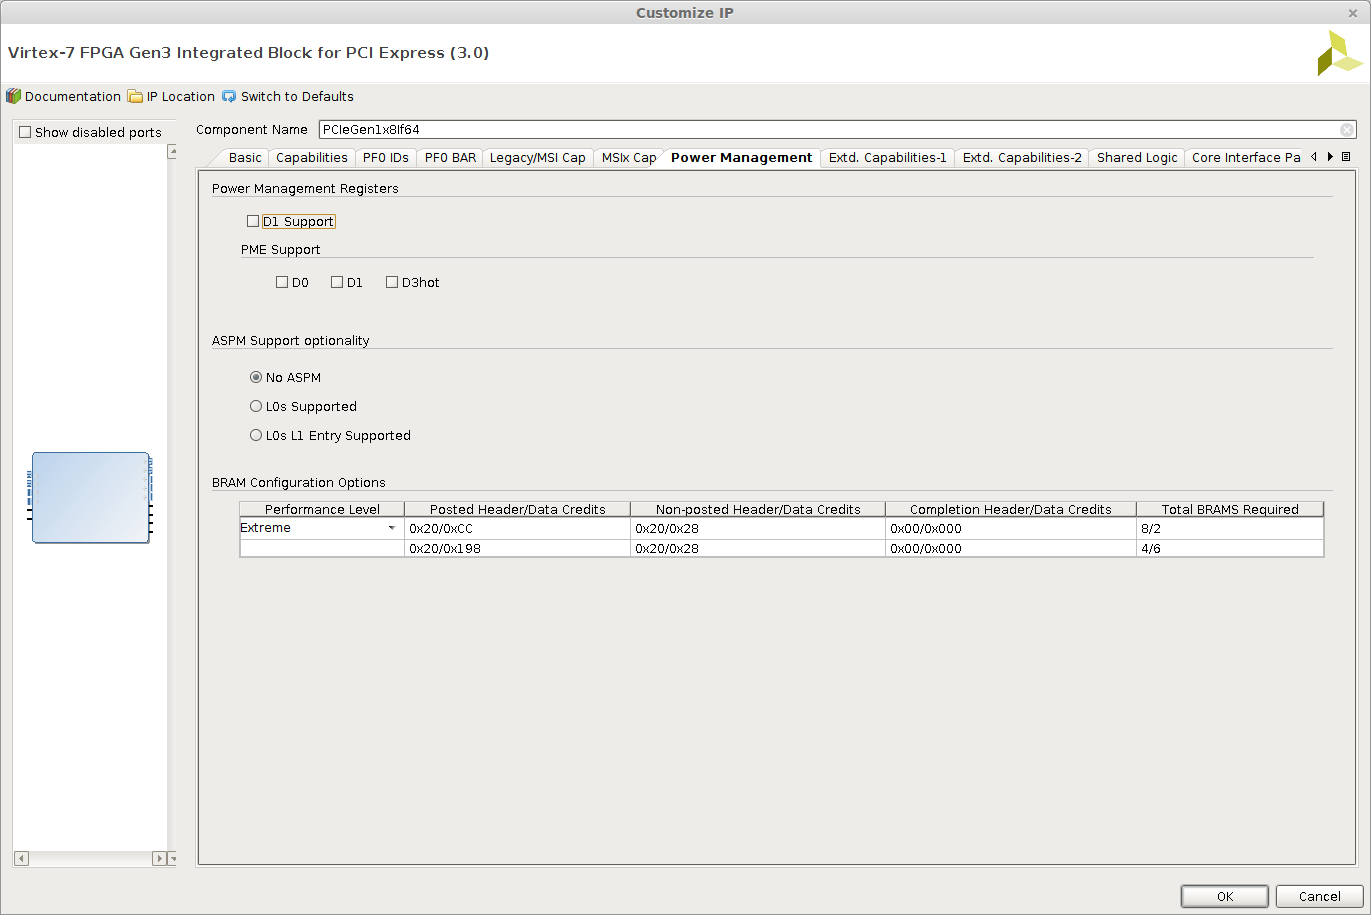
\includegraphics[width=350px,center]{Gen3IntegratedTabPowerManagement.png}
  \caption{PCI Express Power Management Tab.}
  \label{Fig:Gen3Integrated:Generating:Gen3IntegratedTabPowerManagement}
\end{figure}
In the Power Management tab, shown in
Figure~\ref{Fig:Gen3Integrated:Generating:Gen3IntegratedTabPowerManagement},
ensure that the \ConfigSetting{Performance Level} is set to
\ConfigSetting{Extreme}.
% \begin{figure}[H]
%   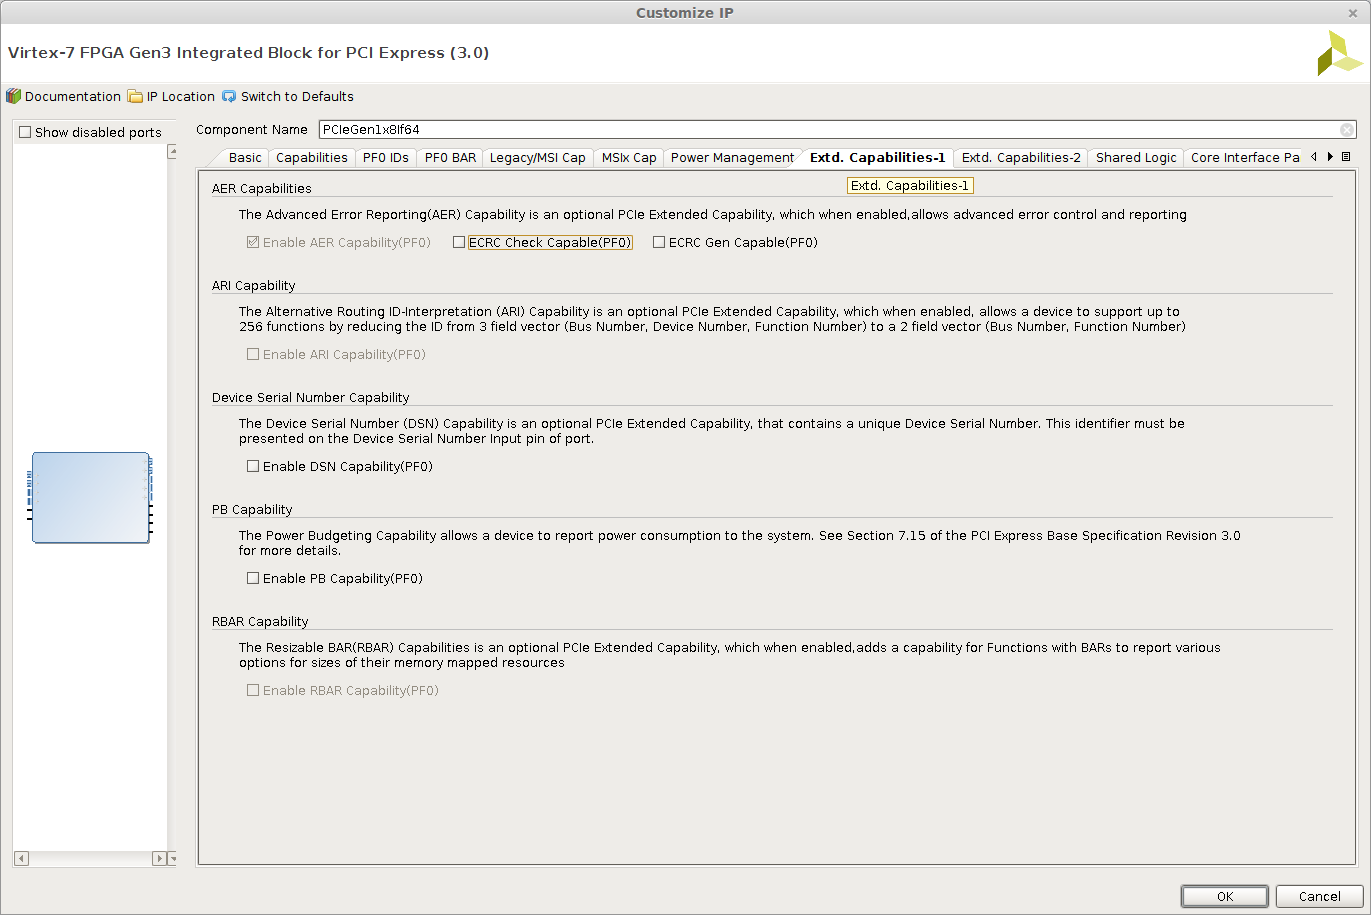
\includegraphics[width=350px,center]{Gen3IntegratedTabExtCapabilities1.png}
%   \label{Fig:Gen3Integrated:Generating:Gen3IntegratedTabExtCapabilities1}
% \end{figure}
% \begin{figure}[H]
%   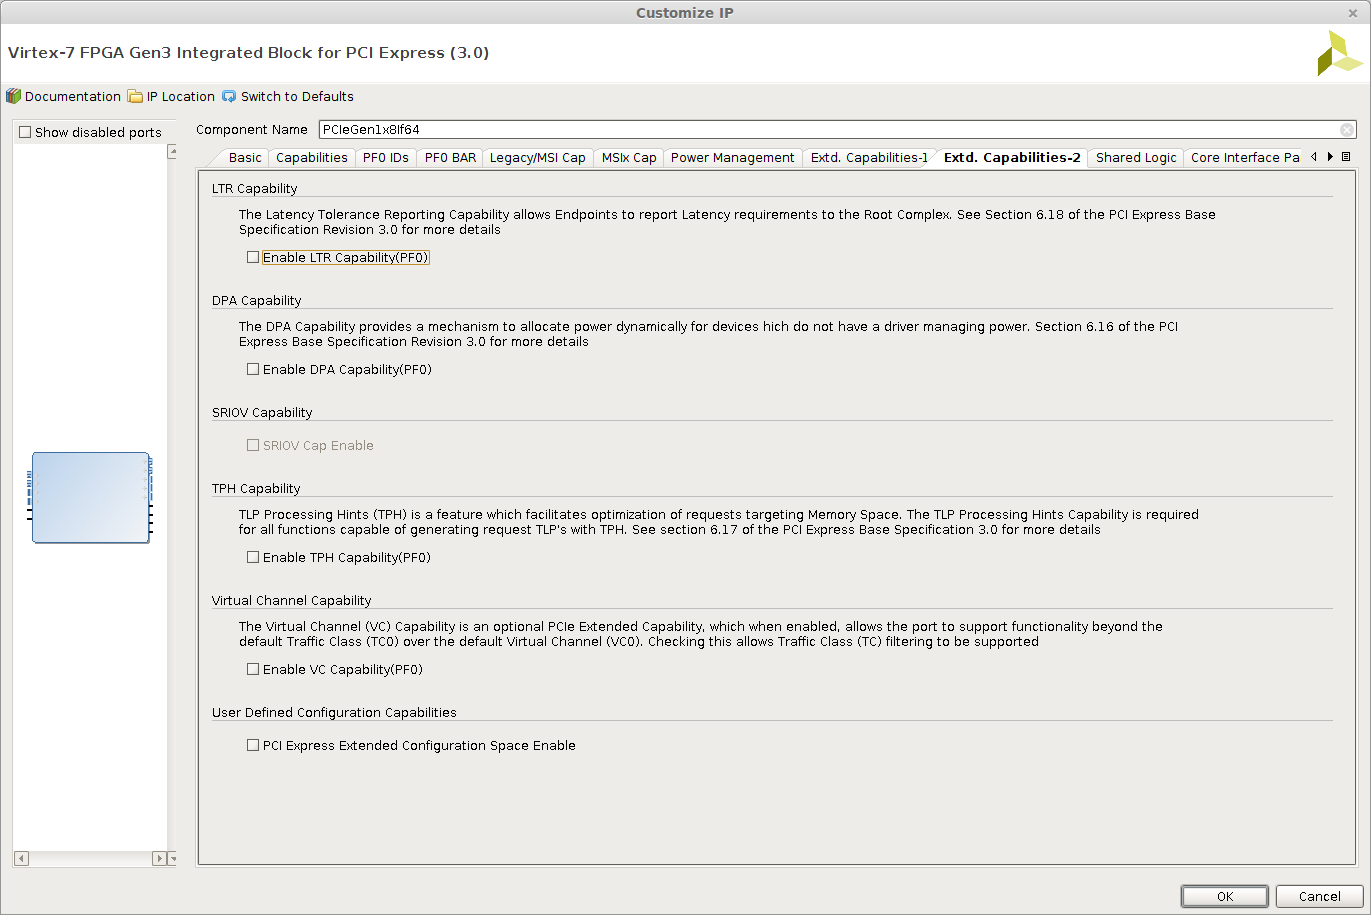
\includegraphics[width=350px,center]{Gen3IntegratedTabExtCapabilities2.png}
%   \label{Fig:Gen3Integrated:Generating:Gen3IntegratedTabExtCapabilities2}
% \end{figure}
\begin{figure}[H]
  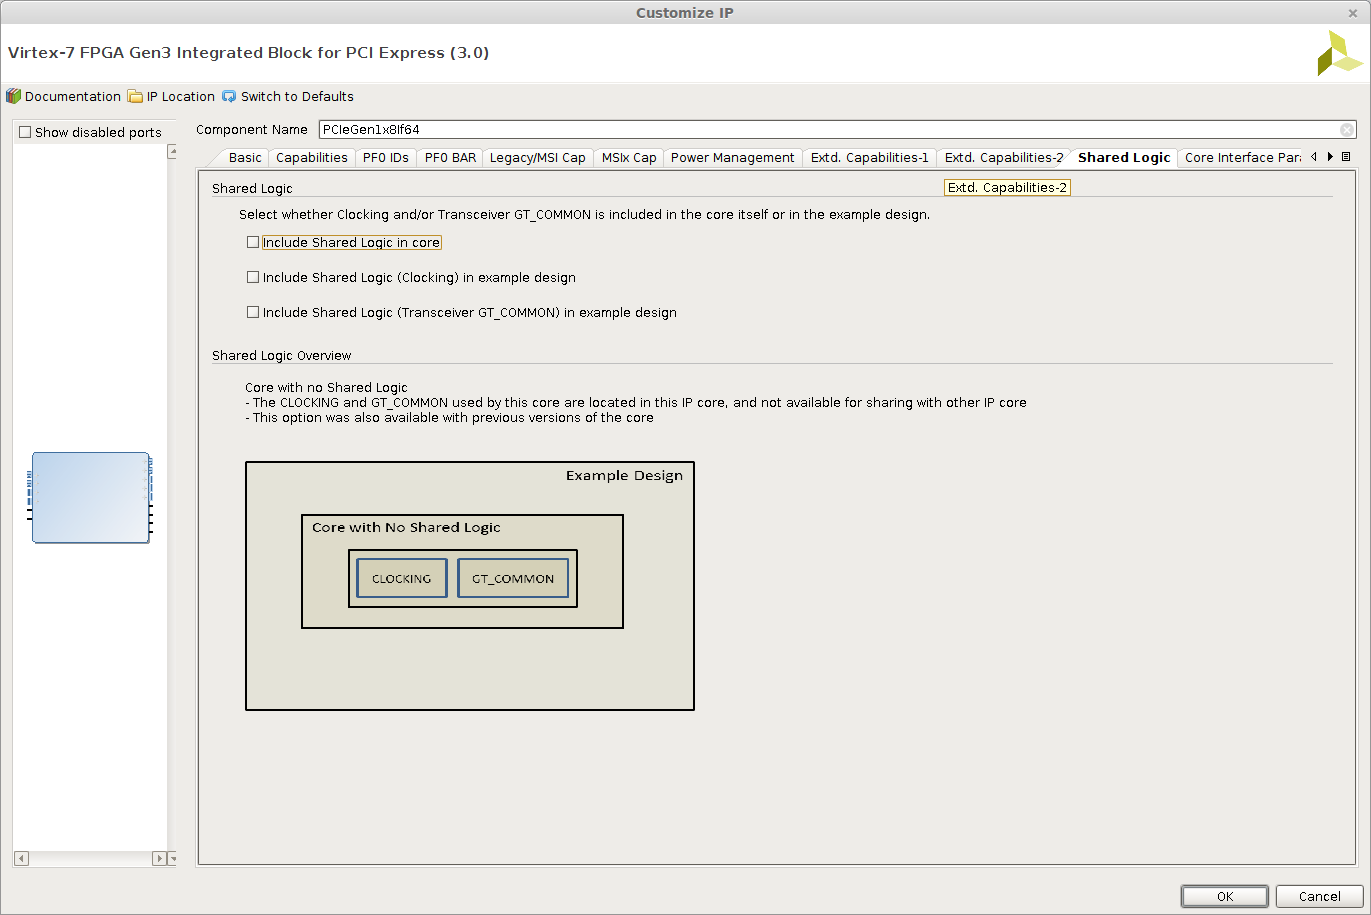
\includegraphics[width=350px,center]{Gen3IntegratedTabSharedLogic.png}
  \caption{PCI Express Shared Logic Tab.}
  \label{Fig:Gen3Integrated:Generating:Gen3IntegratedTabSharedLogic}
\end{figure}
In the Shared Logic Tab shown in
Figure~\ref{Fig:Gen3Integrated:Generating:Gen3IntegratedTabSharedLogic}
\ConfigSetting{clear} all of the checkboxes shown. These settings will not
affect the core generated, but will affect the example designs generated by the
Vivado, and make the Vivado example design mirror the RIFFA Example design.
\begin{figure}[H]
  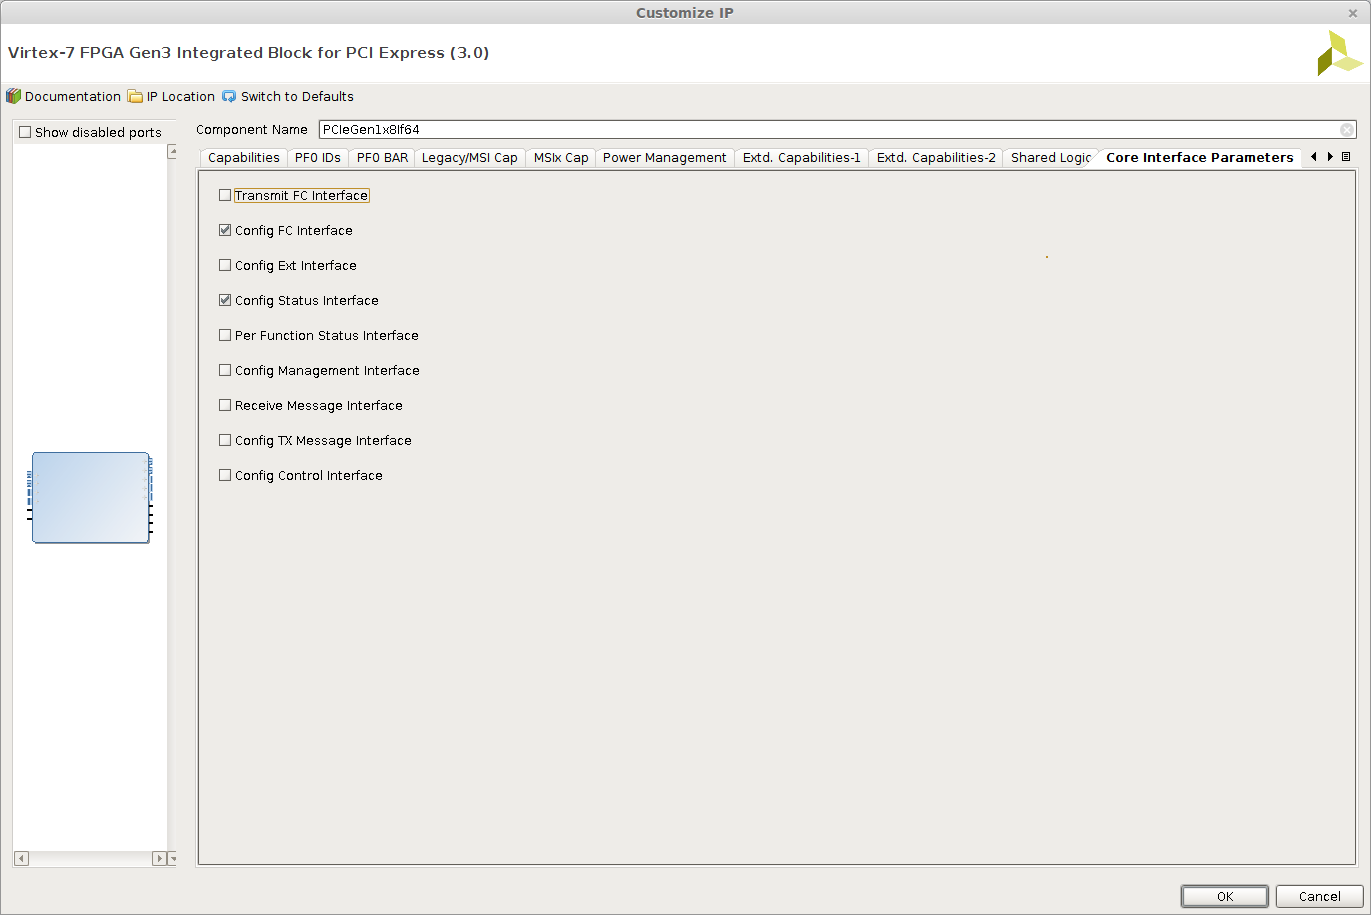
\includegraphics[width=350px,center]{Gen3IntegratedTabCoreInterfaceParameters.png}
  \caption{PCI Express Core Interface Parameters Tab.}
  \label{Fig:Gen3Integrated:Generating:Gen3IntegratedTabCoreInterfaceParameters}
\end{figure}
Finally, in the Interface Parameters tab, match the checkboxes shown in
Figure~\ref{Fig:Gen3Integrated:Generating:Gen3IntegratedTabCoreInterfaceParameters}. These
options simplify the interface to the generated core
\subsection{Creating Constraints files for the VC709 Development Board}
\label{Sec:Gen3Integrated:Generating:Constraints}
When generating a design for the VC709 board, the following constraints will
correctly constrain the clocks. When using a different board, read the user
guide for appropriate pin placment, or copy the constraints from the PCIe
Endpoint Example Design.
\begin{lstlisting}[basicstyle=\footnotesize\ttfamily,language=tcl,
    commentstyle=\color{red},label=Listing:7SeriesIntegrated:Generating:Constraints:VC709,
    caption=\Xilinx{.xdc} constraints for the VC709 board,frame=single]
  create_clock -period 10.000 -name pcie_refclk [get_pins refclk_ibuf/O]
  set_false_path -from [get_ports PCIE_RESET_N]

  # The following constraints are BOARD SPECIFIC. This is for the VC709
  set_property LOC IBUFDS_GTE2_X1Y11 [get_cells refclk_ibuf]
  set_property PACKAGE_PIN AV35 [get_ports PCIE_RESET_N]
  set_property IOSTANDARD LVCMOS18 [get_ports PCIE_RESET_N]
  set_property PULLUP true [get_ports PCIE_RESET_N]
\end{lstlisting}

\pagebreak
\chapter{Compiling and using the Altera Example Designs}
\label{Chap:Altera}
This section describes how to use RIFFA \RIFFAVer~ with Quartus \QuartusVer. The
example projects included in this distribution target Terasic DE5Net and DE4
boards. We are confident that RIFFA will work on all currently supported Altera
devices using the Hard IP for PCI Express (Cyclone V, Arria V and Stratix V)
devices, as well as all devices using IP Compiler for PCI Express (Stratix IV
and prior). For device support in Quartus \QuartusVer
see \footnote{http://dl.altera.com/devices/}

The FPGA families that we have successfully tested RIFFA \RIFFAVer~are:
\begin{itemize}
\item Stratix V (DE5-Net)
\item Stratix IV (DE4)
  %\item Cyclone IV (DE2i-150)
\end{itemize}
There are three options for starting a new RIFFA project:
\begin{itemize}
\item For first-time users with a DE5 board, we recommend the archived projects
  provided in the \Directory{RIFFA \RIFFAVer/source/fpga/de5\_qsys} directory. Follow the
  instructions in Section~\ref{Sec:Altera:QsysMegawizard:Qsys}
\item Intermediate and advanced users, or users with a DE4 board, we have
  provided projects without instantiated IP. For DE5 boards, follow the
  instructions in Section~\ref{Sec:Altera:QsysMegawizard:Megawizard}. For DE4 boards, follow
  the instructions in Section~\ref{Sec:Altera:IPCompiler}
\item For advanced users, or users wishing to support a new board, we provide
  full instructions for creating a top level and generating IP. Follow the
  instructions in Section~\ref{Sec:Altera:QsysMegawizard}
\end{itemize}

\section{Example Designs with Qsys and MegaWizard (Stratix V, Cyclone V and newer)}
\label{Sec:Altera:QsysMegawizard}
\subsection{Qsys (Stratix V and newer)}
\label{Sec:Altera:QsysMegawizard:Qsys}
For first-time users with the DE5-Net board, copy one of the archived projects
(.qar files) available in the \Directory{de5\_qsys} directory.

\begin{enumerate}
\item Open Quartus to get the introductory screen shown in
  Figure~\ref{Fig:Quartus:WelcomeScreen}.
\item Click 'Open an Existing Project' and navigate to your RIFFA
  \RIFFAVer~directory.
\item In the RIFFA \RIFFAVer~distribution, open \Directory{RIFFA
  \RIFFAVer/source/fpga/de4/} and choose from one of the existing example design
  directories for your board. In the example design directory, locate the
  \Directory{prj} folder and open it. Select the .qpf file and click open. This
  will open the example project, as shown in
  Figure~\ref{Fig:Quartus:ExampleDesign:ProjectOpened}.
\item This project was compiled in Quartus \QuartusVer. The bit file generated
  can be used to test the FPGA system. If you are using a newer version of
  Quartus, recompile the example design or use the programming file provided.
  \begin{itemize}
  \item To recompile the example design, click the compile button in the top
    left corner as shown in
    Figure~\ref{Fig:Quartus:ExampleDesign:ProjectOpened}.
  \item Recompiling your design will generate a new bitfile in the
    \Directory{prj} directory. The bit file in the \Directory{bit} will not be
    changed.
  \end{itemize}
\item To program the FPGA, click 'Open Programmer'. New bit files (generated by
  Quartus) will appear in the \Directory{prj/output\_files/} directory. An example
  bit file is provided in the example design's \Directory{bit} directory.
  \begin{itemize}
  \item Before programming your FPGA, you should install the RIFFA driver. See
    Section~\ref{Sec:RIFFA:Installation}
  \end{itemize}
\item The example design uses the chnl\_tester (shown in
  Figure~\ref{Fig:Quartus:ExampleDesign:chnl_tester}, which works with
  the example software in the \Directory{source/\{C\_C++,Java,python,matlab\}}
  directories. Replace the chnl\_tester instantiation with any user logic,
  matching the RIFFA interface.
\item Recompile the design and program the FPGA Device. Changing the
  \RIFFAParameter{C\_NUM\_CHNL} will change the number of independent channel
  interfaces
\end{enumerate}
\begin{figure}
  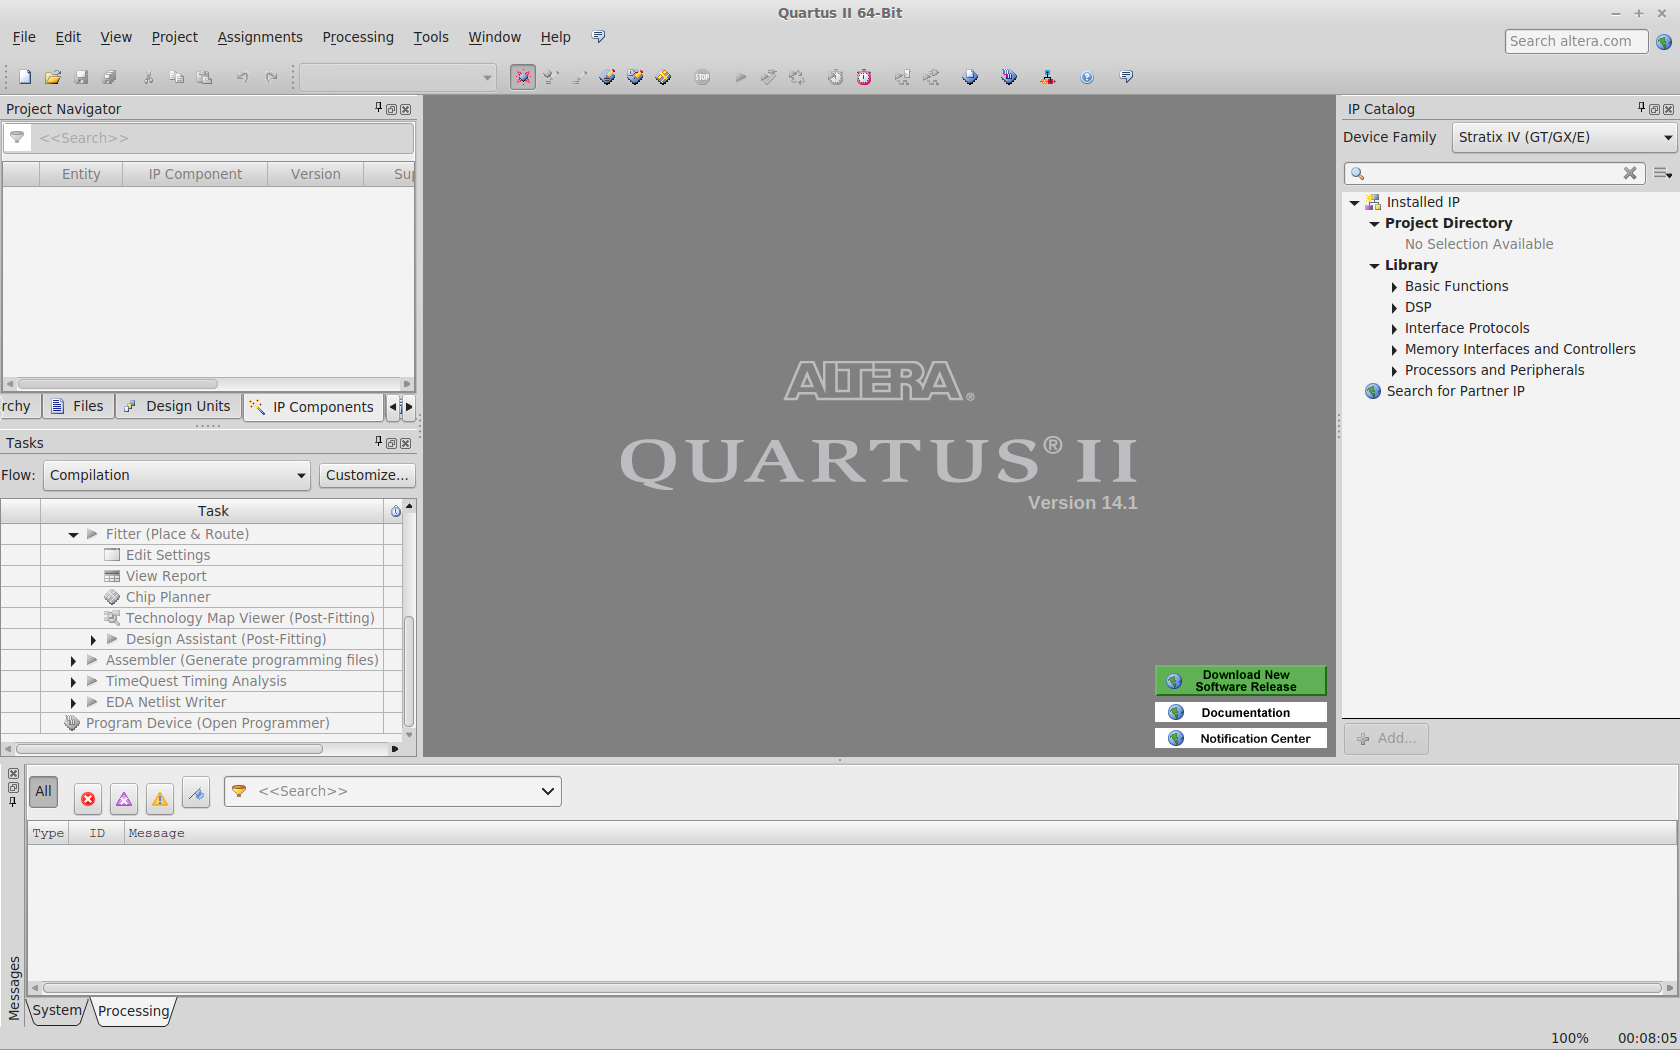
\includegraphics[width=300px,center]{QuartusWelcomeScreen.png}
  \caption{Welcome Screen for Quartus \QuartusVer}
  \label{Fig:Quartus:WelcomeScreen}
\end{figure}
\begin{figure}
  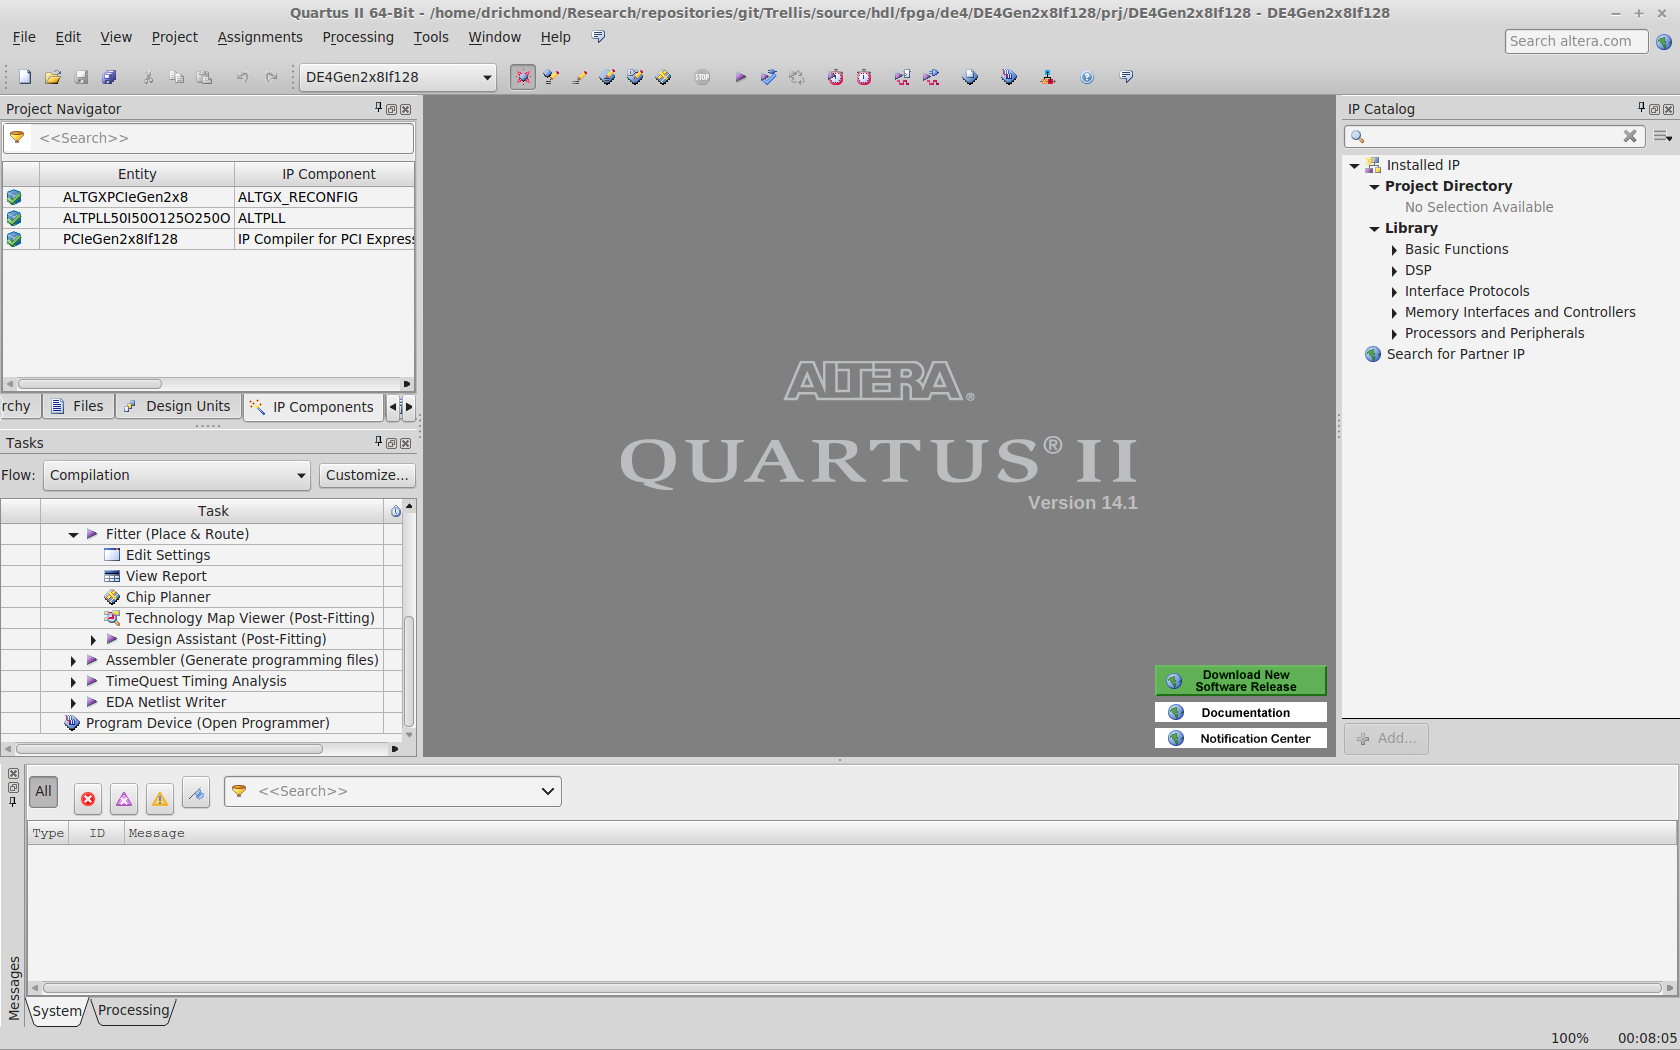
\includegraphics[width=300px,center]{IPCompileOpenProject.png}
  \caption{Project Splash Screen for Quartus Projects}
  \label{Fig:Quartus:ExampleDesign:ProjectOpened}
\end{figure}
\begin{figure}
  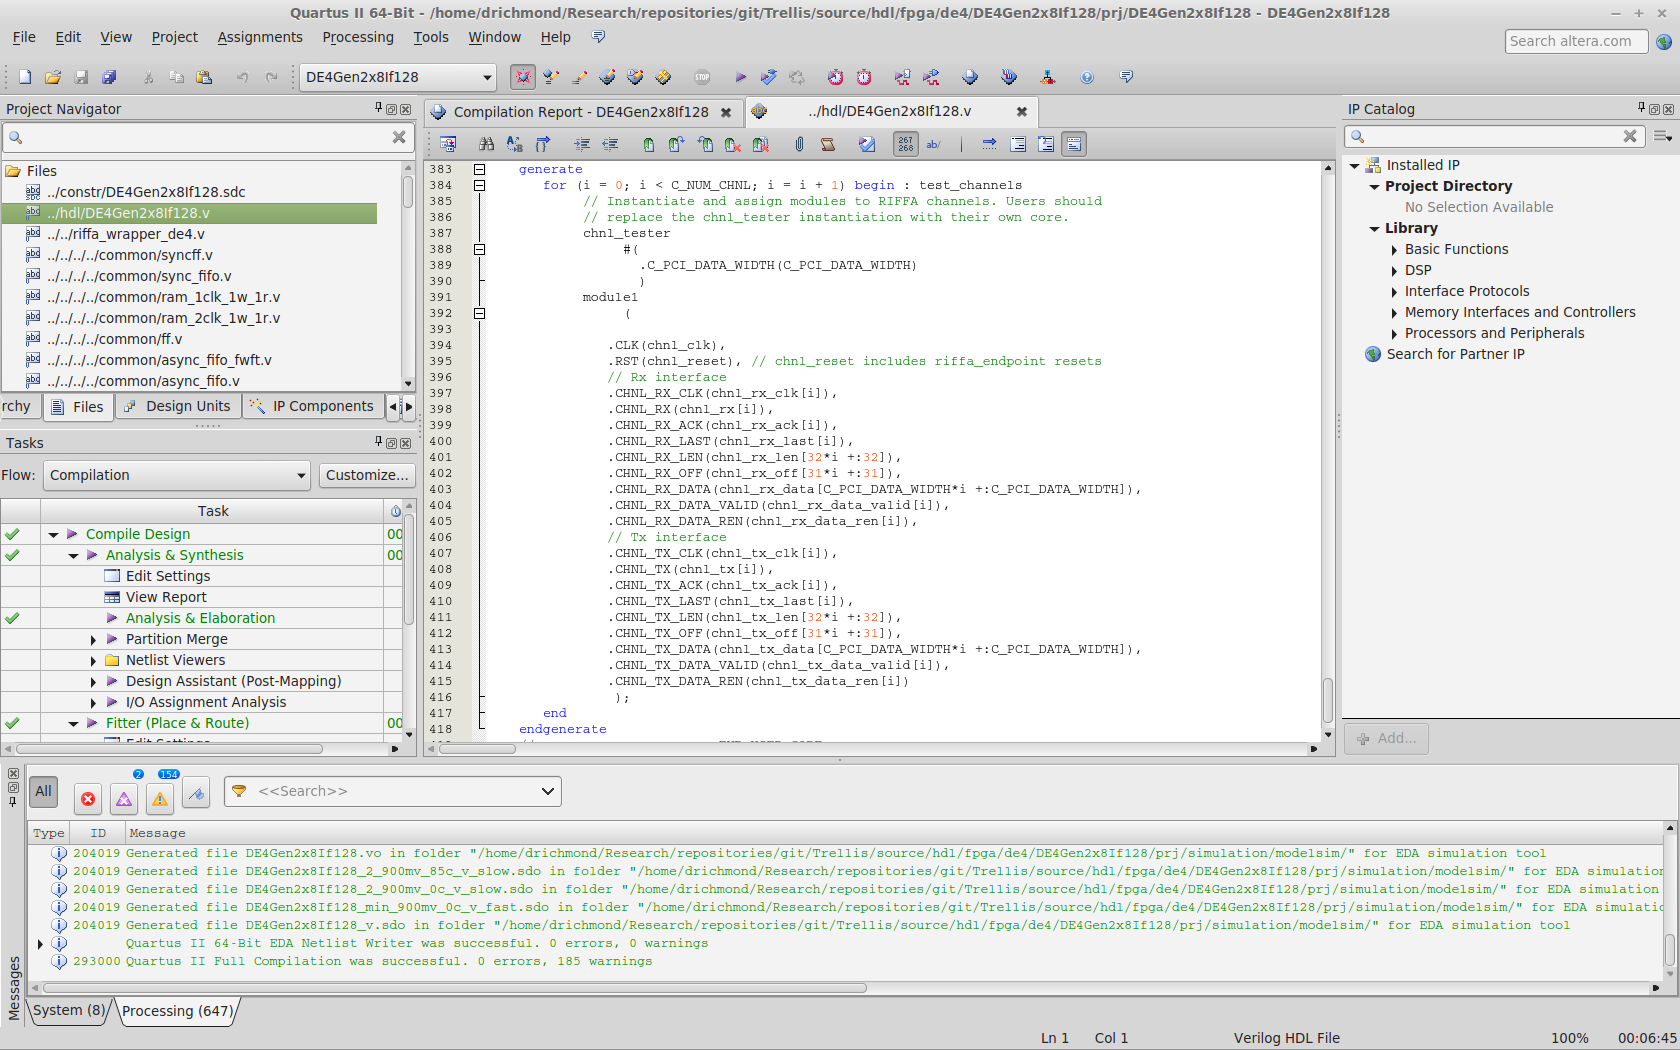
\includegraphics[width=300px,trim=400 200 300 200, clip=true,center]{QuartusChnlTesterInstantiation.png}
  \caption{chnl\_tester instantiation in the top level file}
  \label{Fig:Quartus:ExampleDesign:chnl_tester}
\end{figure}

\subsection{Generating IP using MegaWizard (Stratix V, Cyclone V and newer)}
\label{Sec:Altera:QsysMegawizard:Megawizard}
In some cases, it may be necessary to generate the PCIe Endpoint IP. For
intermediate users, there are project example projects inside of the
\Directory{de5} directory without instantiated IP (This is done to avoid
licensing problems). For the DE5, the project directories are: DE5Gen1x8If64,
DE5Gen2x8If128, DE5Gen3x4If128.

Modifying the RIFFA parameters \RIFFAParameter{C\_PCI\_DATA\_WIDTH},
\RIFFAParameter{C\_MAX\_PAYLOAD\_BYTES} and \RIFFAParameter{C\_LOG\_NUM\_TAGS}
require changing certain settings in the IP core file. The paramter
\RIFFAParameter{C\_NUM\_LANES} is located in the top level file of each example
project. How these parameters relate to IP core settings is highlighted in the
following figures.

For advanced users whose goal is to generate a RIFFA design completely from
scratch, we provide instructions for generating the timing constraints and other
low level details. Each board directory contains with a RIFFA wrapper verilog
file and instantiates a vendor-specific translation layer. It is highly
recommended to re-use these files RIFFA wrapper when creating designs from
scratch. Users should also use the constraints file (\Altera{.sdc}) in the board
directory, and in the \Directory{constr/}, or read the User Guide provided with
each board and the instructions for generating constratints in
Section~\ref{Sec:Altera:QsysMegawizard:Constraints}.

As stated in Section~\ref{Sec:Intro:Decoding}, each project directory contains five folders.
\begin{itemize}
\item The \Directory{prj/} directory contains the project \Altera{.qpf} and \Altera{.qsf} file.
\item The \Directory{hdl/} contains the top level file, e.g. DE5Gen2x8If128.v, which instantiates the skeleton IP and the RIFFA Core.
\item The \Directory{ip/} directory is empty but will contain Altera IP generated by Quartus
  in the following guide.
\item The \Directory{constr/} directory contains project-specific timing constraint files.
\item Finally the \Directory{bit/} directory contains the project .sof, or bit
  file that we have tested. This bitfile will not be overwritten by subsequent Quartus compilations.
\end{itemize}

Note: The bitfile in the bit directory is not modified by recompilation in
Quartus. Quartus will generate a new bitfile (.sof) in the \Directory{prj/}
directory for the DE5Net board.

\begin{figure}[H]
  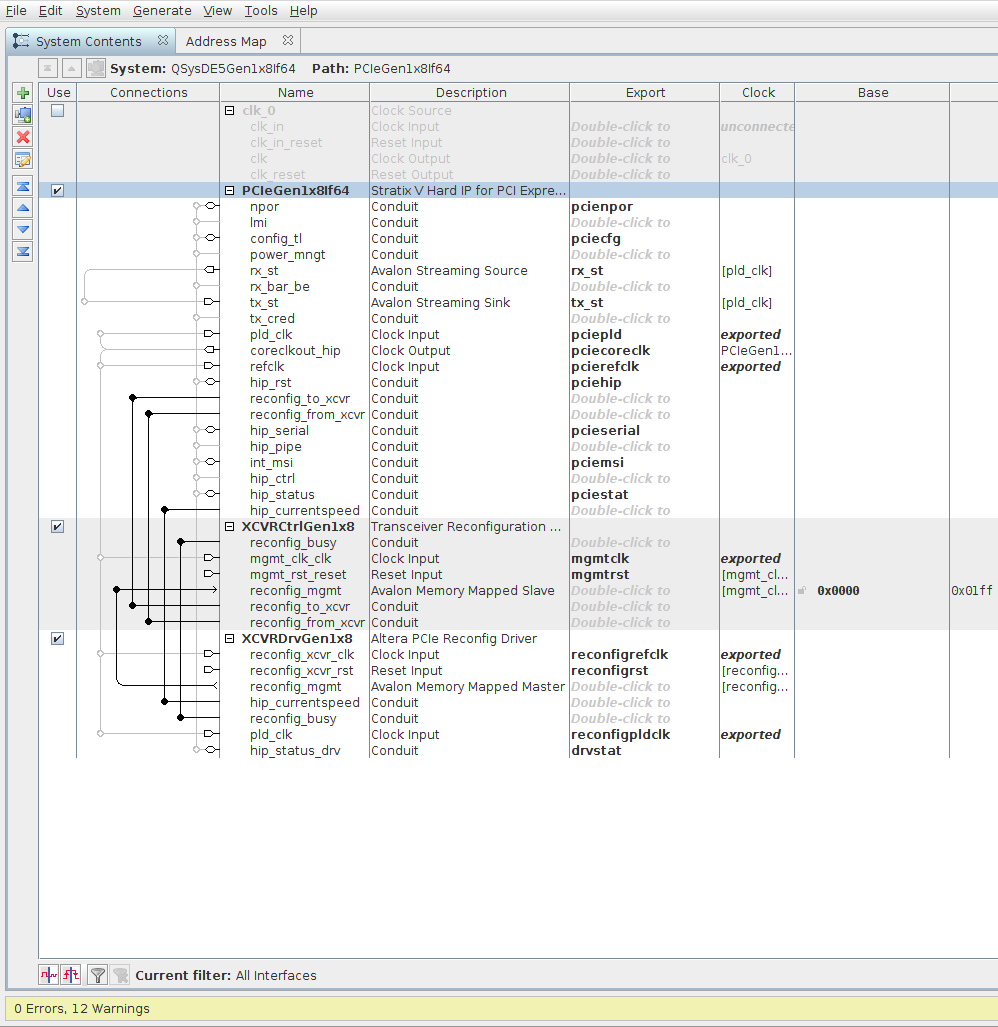
\includegraphics[width=350px,center]{QsysPCIExpSystemTrim.png}
  \caption{Qsys Diagram depicting the connections between the three Altera IP blocks.}
  \label{Fig:Altera:QsysMegawizard:Megawizard:QsysPCIExpSystemTrim}
\end{figure}

Altera designs require additional IP to drive the PCIe Core Transcievers. For the
DE5, these blocks are the Transciever Reconfiguration Controller and the
Reconfiguration Driver. When creating a new top level design, these blocks must be
connected together with the PCIe Endpoint as shown in
Figure~\ref{Fig:Altera:QsysMegawizard:Megawizard:QsysPCIExpSystemTrim}.

First, we will generate the PCIe Endpoint. Click on the Avalon Streaming
Interface for PCI Express in the Quartus IP Catalog.
Figure~\ref{Fig:Altera:IPCompiler:PCIeSystemSettingsTab}.

Optional: Set the Component Name of the PCI Express block, and the IP
Location. In our example projects, we typically use the name
PCIeGen\textbf{W}x\textbf{Y}If\textbf{Z} where \textbf{W} is the PCI Express
Version (\ConfigSetting{Link Speed} in
Figure~\ref{Fig:Gen3Integrated:Generating:Gen3IntegratedTabBasic}), \textbf{Y}
is the lane width, and \textbf{Z} is the Avalon interface width. The IP location
is the \Directory{ip/} directory in the example project.

\begin{figure}[H]
  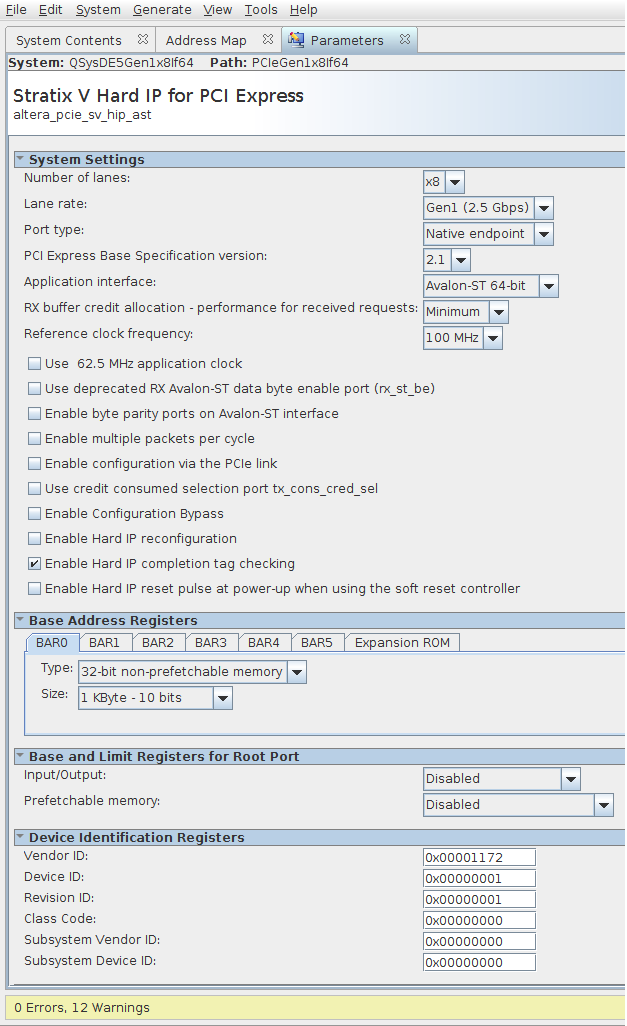
\includegraphics[width=350px,center]{PCIExpressEndpoint1Trim.png}
  \caption{PCI Express Endpoint Configuration Menu}
  \label{Fig:Altera:QsysMegawizard:Megawizard:PCIExpressEndpoint1Trim}
\end{figure}

In Figure~\ref{Fig:Altera:QsysMegawizard:Megawizard:PCIExpressEndpoint1Trim},
select the \ConfigSetting{Number of Lanes}, which corresponds to the top level
parameter \RIFFAParameter{C\_NUM\_LANES}, \ConfigSetting{Lane Rate}, and
\ConfigSetting{PCI Express Base Specification} version from the dropdown menus
(Choose the highest possible base specification version). Select an
\ConfigSetting{Application Interface Width}; This corresponds to the
\RIFFAParameter{C\_PCI\_DATA\_WIDTH} parameter in RIFFA. Currently the
\ConfigSetting{64-bit} and \ConfigSetting{128-bit} interfaces are supported for
all Altera designs. Some widths may not be possible depending on the
\ConfigSetting{Lane Rate} and \ConfigSetting{Number of Lanes} selected.

The choice of \ConfigSetting{Link Rate}, \ConfigSetting{Number of Lanes}, and
\ConfigSetting{Interface Width} will set the frequency for the PCI interface,
which is clocked by the pld\_clk signal. For the chosen settings, the frequency
should be displayed in the messages bar at the bottom of the configuration menu
(Messages bar not shown). The RIFFA core will run at this clock frequency, but the
user logic can run at whatever frequency it desires.

In the Base Address Registers Section set BAR0's type to \ConfigSetting{32-bit
  non-prefetchable memory} and set the size to \ConfigSetting{1 KByte - 10 Bits}.

There are no required changes in the Device Identification Registers
Section. However, in a multiple FPGA system, it may be useful to change the
\ConfigSetting{Device ID} to allow identification of different FPGA
platforms. The other options, specifically the \ConfigSetting{Vendor ID}, must
remain the same.

Scroll down to view the final two sections shown in
Figure~\ref{Fig:Altera:QsysMegawizard:Megawizard:PCIExpressEndpoint2Trim}.
\begin{figure}[H]
  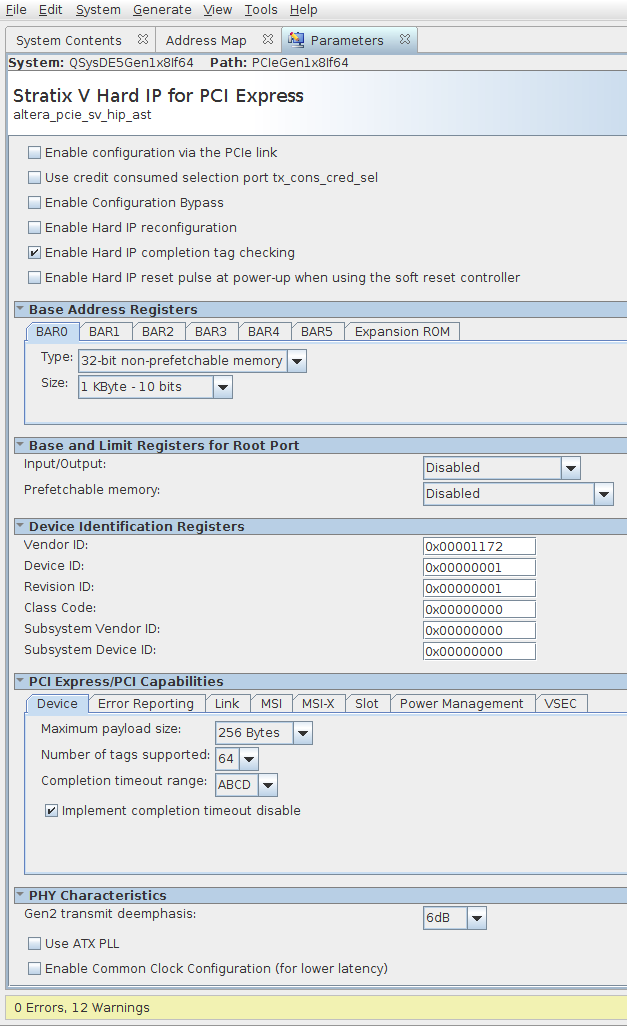
\includegraphics[width=350px,trim=0 0 0 620, clip=true,center]{PCIExpressEndpoint2Trim.png}
  \caption{PCI Express Endpoint Configuration Menu}
  \label{Fig:Altera:QsysMegawizard:Megawizard:PCIExpressEndpoint2Trim}
\end{figure}
In the PCI Express/PCI Capabilities menu, set your desired
\ConfigSetting{Maximum Payload Size}, which corresponds to the RIFFA parameter,
\RIFFAParameter{C\_MAX\_PAYLOAD\_BYTES} and the \ConfigSetting{Number of Tags
  Supported}. The log of the \ConfigSetting{Number of Tags Supported} is
the \RIFFAParameter{C\_LOG\_NUM\_TAGS} parameter in RIFFA.

In the MSI Tab, make sure that the number of MSI messages requested is equal to
1.

Note: Maximum Payload sizes are typically set by the BIOS, and 256 bytes seems
to be standard. RIFFA will default to the minimum setting
\RIFFAParameter{C\_MAX\_PAYLOAD\_SIZE} and the setting in your BIOS. Unless your
BIOS is modified, or can support substantially larger packets, there will be no
performance benefit to increasing the payload size. Increasing the
\ConfigSetting{Maximum Payload Size} will increase the resources consumed.

Finally, record the number of \ConfigSetting{Transciever Reconfiguration
  Interfaces} in the messages bar at the bottom of the screen, then close the
PCIe IP Generation Menu. A window may ask if you wish to generate the example
design. This is optional.
\begin{figure}[H]
  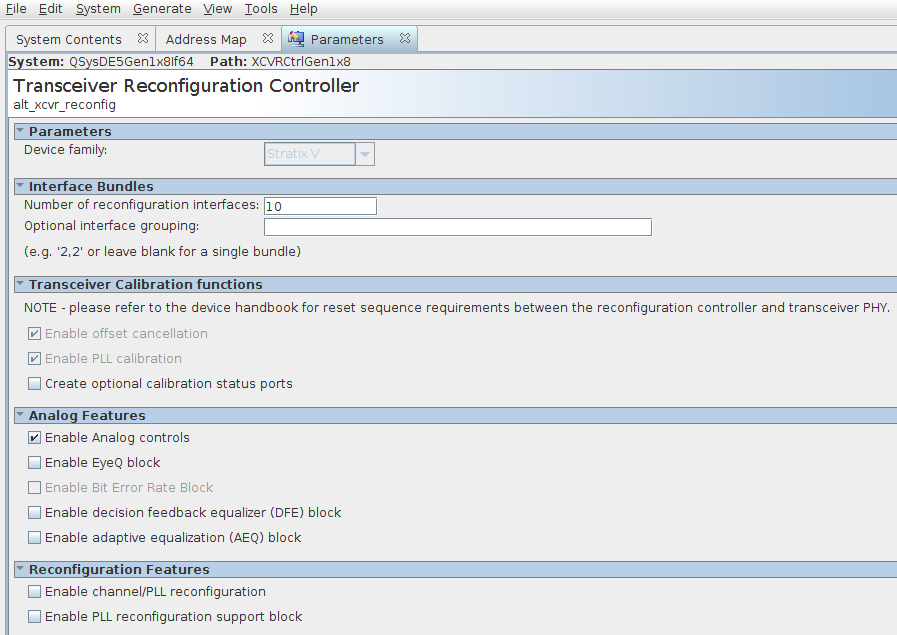
\includegraphics[width=350px,center]{XCVRMenuTrim.png}
  \caption{Transciever Reconfiguration IP Generation Menu}
  \label{Fig:Altera:QsysMegawizard:Megawizard:XCVRMenuTrim}
\end{figure}
Next, generate the Transceiver Reconfiguration Controller by opening MegaWizard
and selecting the Transceiver Reconfiguration Controller megafunction.

Set the appropriate number of \ConfigSetting{Transciever Reconfiguration
  Interfaces} in the Interface Bundles Menu. In the analog features section,
\ConfigSetting{Enable Analog Controls} and \ConfigSetting{Enable Adaptive
  Equalization} block by clicking the appropriate boxes.

Optional: Set the Component Name of the Transciever Reconfiguration Controller, and the IP
Location. In our example projects, we typically use the name
XCVRCtrlGen\ConfigSetting{W}x\ConfigSetting{Y} where \ConfigSetting{W} is the \ConfigSetting{PCI Express Version}
(\ConfigSetting{Link Speed} in
Figure~\ref{Fig:Altera:QsysMegawizard:Megawizard:PCIExpressEndpoint1Trim}), \ConfigSetting{Y}
is the lane width. The IP location is the \Directory{ip/} directory in the
example project.

\begin{figure}[H]
  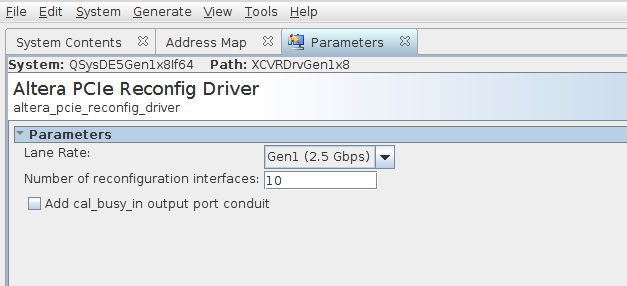
\includegraphics[width=350px,center]{ReconfigDriverMenu.png}
  \caption{Transciever Reconfiguration Driver Menu}
  \label{Fig:Altera:QsysMegawizard:Megawizard:ReconfigDriverMenu}
\end{figure}

In Qsys, generate the Transciver Reconfiguration Controller. Select the
appropriate lane rate for your design, and the number of Reconfiguration
Intefaces. These should match the number of reconfiguration interfaces dictated
when generating the PCIe IP in
Figure~\ref{Fig:Altera:QsysMegawizard:Megawizard:PCIExpressEndpoint1Trim} and
the number selected in
Figure~\ref{Fig:Altera:QsysMegawizard:Megawizard:XCVRMenuTrim}.

Optional (in Qsys): Set the Component Name of the Transciever Reconfiguration
Driver, and the IP Location. In our example projects, we typically use the name
XCVRDrvGen\ConfigSetting{W}x\ConfigSetting{Y} where \ConfigSetting{W} is the
\ConfigSetting{PCI Express Version} (\ConfigSetting{Link Speed} in
Figure~\ref{Fig:Gen3Integrated:Generating:Gen3IntegratedTabBasic}), and
\textbf{Y} is the lane width. The IP location is the \Directory{ip} directory in
the example project.

If you are using Megawizard to instantiate IP, you must manually instantiate the
Transciver Reconfiguration Driver in the Top Level design. The instantiation
template is shown in
Listing~\ref{Listing:Altera:QsysMegawizard:ManualDriverInst} into your top-level
file.  Match the PCIe generation, and chip generation for your project.
\begin{lstlisting}[basicstyle=\footnotesize\ttfamily,language=Verilog,
    commentstyle=\color{red},label=Listing:Altera:QsysMegawizard:ManualDriverInst,
    caption=Manual (non-qsys) instantiation of Reconfiguration Driver,frame=single]
  altpcie_reconfig_driver
  #(
  /* These values should match the values used for the PCIe Endpoint */
  .number_of_reconfig_interfaces(10), /*Set This*/
  .gen123_lane_rate_mode_hwtcl(``Gen1 (2.5 Gbps)''), /*Set This*/
  .INTENDED_DEVICE_FAMILY(``Stratix V'')) /*Set This*/
  XCVRDriverGen2x8_inst
  (
  /*Ports Here -- Copy from Example Designs*/
  );
\end{lstlisting}

\pagebreak
\subsection{Creating Constraints files for MegaWizard and QSys Designs}
\label{Sec:Altera:QsysMegawizard:Constraints}
Advanced users may also want to edit and modify the constraint files. This not
required or recommended for novice users. The example designs in the RIFFA
\RIFFAVer~distribution contain appropriate constraint files for the example
designs. However if the need arises, these constraints are documented below.

To appropriately constrain your PCIe reference clocks, place the constraints
shown in Listing~\ref{Listing:Altera:QsysMegawizard:Constraints} in your
\Altera{.sdc} file. Modify the names PCIE\_REFCLK, PCIE\_TX\_OUT and
PCIE\_RX\_IN to match your design.
\begin{lstlisting}[basicstyle=\footnotesize\ttfamily,language=tcl,
    commentstyle=\color{red},label=Listing:Altera:QsysMegawizard:Constraints,
    caption=\Altera{.sdc} constraints for Qsys and Megawizard designs,frame=single]
  create_clock -name PCIE_REFCLK -period 10.000 [get_ports {PCIE_REFCLK}]
  derive_pll_clocks -create_base_clocks
  derive_clock_uncertainty
\end{lstlisting}
Likewise, copy the constraints in
Listing~\ref{Listing:Altera:QsysMegawizard:QSFSettings} into your .qsf file. Copy
the location assignment commands for each PCIe Pin in your reference design.

\begin{lstlisting}[language=tcl,basicstyle=\footnotesize\ttfamily,commentstyle=\color{red},
    label=Listing:Altera:QsysMegawizard:QSFSettings,
    caption=\Altera{.qsf} settings for Qsys and Megawizard designs,frame=single]
  ###################################################################
  # PCIE Connections
  ###################################################################
  set_location_assignment <PCIE_REFCLK_PIN> -to PCIE_REFCLK
  set_instance_assignment -name IO_STANDARD HCSL -to PCIE_REFCLK
  set_location_assignment <PCIE_REFCLK_PIN(n)> -to ``PCIE_REFCLK(n)''
  set_instance_assignment -name IO_STANDARD HCSL -to ``PCIE_REFCLK(n)''
  set_location_assignment <PCIE_RESET_N> -to PCIE_RESET_N
  set_instance_assignment -name IO_STANDARD ``2.5 V'' -to PCIE_RESET_N

  # For each PCIE Lane (L) set the pin locations from the board user guide!
  ######################################################################
  #PCIE TX_OUT L
  ######################################################################
  set_location_assignment <TX_LANE[L]_PIN>   -to PCIE_TX_OUT[0]
  set_location_assignment <TX_LANE[L]_PIN(n)> -to ``PCIE_TX_OUT[0](n)''

  ###################################################################
  #PCIE RX_IN L
  ###################################################################
  set_location_assignment <RX_LANE[L]_PIN>  -to PCIE_RX_IN[L]
  set_location_assignment <RX_LANE[L]_PIN(n)> -to ``PCIE_RX_IN[L](n)''
\end{lstlisting}
\pagebreak

\section{IP Compiler for PCI Express (Stratix IV, and older)}
\label{Sec:Altera:IPCompiler}
To avoid licensing problems, we do not package Altera IP for the DE4
board. Manual IP Instantiation is required when using the DE4 Board, and similar
devices using the IP Compiler for PCI Express. Changing the endpoint settings
described here may change the RIFFA para\-meters
\RIFFAParameter{C\_PCI\_DATA\_WIDTH}, \RIFFAParameter{C\_MAX\_PAYLOAD\_BYTES}
and \RIFFAParameter{C\_LOG\_NUM\_TAGS}. How these parameters relate to IP core
settings is highlighted in the following figures.

There are sever example projects inside of the \Directory{de4} directory folder
without instantiated IP. For the DE4 board, these
projects are DE4Gen1x8If64, DE4Gen2x8If128.% and DE2Gen1x1If64 for the DE2i-150
board.

As stated in Section~\ref{Sec:Intro:Decoding}, each project directory contains
five folders.
\begin{itemize}
\item The \Directory{prj/} directory contains the project \Altera{.qpf} and \Altera{.qsf} file.
\item The \Directory{hdl/} contains the top level file, e.g. DE5Gen2x8If128.v,
  which instantiates the skeleton IP and the RIFFA Core.
\item The \Directory{ip/} directory is empty but will contain Altera IP generated by Quartus
  in the following guide.
\item The \Directory{constr/} directory contains project-specific timing constraint files.
\item Finally the \Directory{bit/} directory contains the project .sof, or bit
  file that we have tested. This bitfile will not be overwritten by subsequent
  Quartus compilations.
\end{itemize}

\subsection{Generating IP with IP Compiler for PCI Express (Stratix IV, and older)}
\label{Sec:Altera:IPCompiler:Generating}
Note: The bitfile in the bit directory is not modified by recompilation in
Quartus. Quartus will generate a new bitfile (.sof) in the
\Directory{/output\_files} directory for the DE4 board.

First, we will generate the PCIe Endpoint. Open the Altera IP Catalog and select
the IP Compiler for PCI Express. This will open the window shown in
Figure~\ref{Fig:Altera:IPCompiler:PCIeSystemSettingsTab}.

Optional: Set the Component Name of the PCI Express block, and the IP
Location. In our example projects, we typically use the name
PCIeGen\ConfigSetting{W}x\ConfigSetting{Y}If\ConfigSetting{Z} where \ConfigSetting{W} is the PCI Express
Version (Link Speed in
Figure~\ref{Fig:Gen3Integrated:Generating:Gen3IntegratedTabBasic}), \ConfigSetting{Y}
is the lane width, and \ConfigSetting{Z} is the Avalon interface width. The IP location
is the \Directory{ip} directory in the example project.

In this guide, we will skip the Power Mangement tab shown in
Figure~\ref{Fig:Altera:IPCompiler:PCIeSystemSettingsTab}.
\begin{figure}[H]
  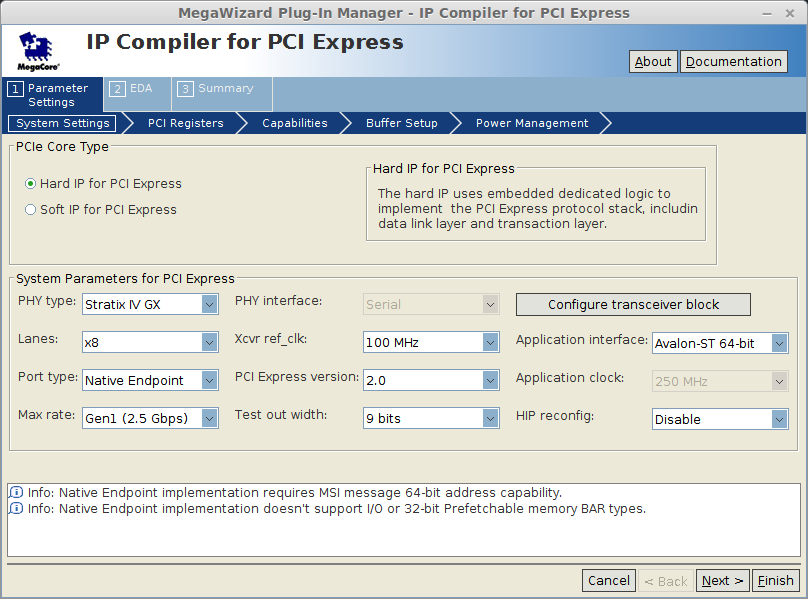
\includegraphics[width=350px,center]{IPCompilerPCIeTabSystemSettings.png}
  \caption{IP Compiler for PCI Express System Settings Tab}
  \label{Fig:Altera:IPCompiler:PCIeSystemSettingsTab}
\end{figure}
In the first column of the System Settings Tab, select your \ConfigSetting{Chip
  Generation/PHY Type} (\ConfigSetting{Stratix IV GX} for the DE4 board),
\ConfigSetting{Lanes}, and \ConfigSetting{Max Rate}. The \ConfigSetting{Number
  of Lanes} is the parameter \RIFFAParameter{C\_NUM\_LANES} in the project top
level file. In the second column, select the \ConfigSetting{PCI Express Version}
(2.0, or the highest possible) and set the \ConfigSetting{Test Out Width} to
\ConfigSetting{0}. In the third column, select the \ConfigSetting{Application Interface
  Width}. The \ConfigSetting{Application Interface Width} corresponds to the RIFFA parameter
\RIFFAParameter{C\_PCI\_DATA\_WIDTH}.

The choice of \ConfigSetting{Link Rate}, \ConfigSetting{Lanes}, and
\ConfigSetting{Interface Width} will set the frequency for the PCI interface,
which is clocked by the signal pld\_clk. For the chosen settings, the frequency
is determined in the Chip User Guide (though, typically it is one of 62.5, 125,
or 256 MHz)

\begin{figure}[H]
  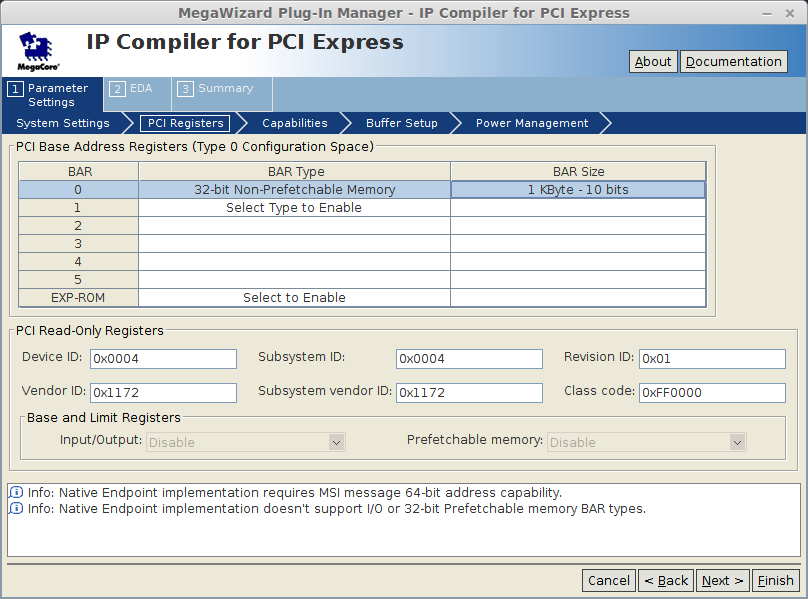
\includegraphics[width=350px,center]{IPCompilerPCIeTabPCIRegisters.png}
  \caption{IP Compiler for PCI Express Registers Tab}
  \label{Fig:Altera:IPCompiler:PCIRegisters}
\end{figure}
PCI Registers Tab, shown in Figure~\ref{Fig:Altera:IPCompiler:PCIRegisters}, set
BAR0's type to ``32-bit non-prefetchable memory''. Set the size to ``1 KByte -
10 Bits''.

There are no required changes in the PCI Registers Tab. However, in a multiple
FPGA system, it may be useful to change the \ConfigSetting{Device ID} to
identify different FPGA platforms. The other options, specifically the
\ConfigSetting{Vendor ID}, must remain the same.
\begin{figure}[H]
  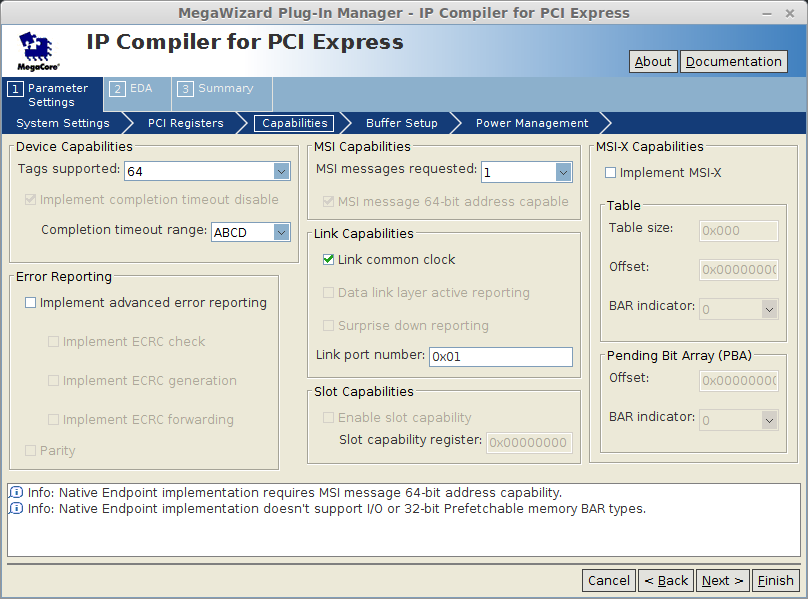
\includegraphics[width=350px,center]{IPCompilerPCIeTabCapabilities.png}
  \caption{IP Compiler for PCI Express Capabilities Tab}
  \label{Fig:Altera:IPCompiler:PCIeCapabilitiesTab}
\end{figure}
Open the Capabilities Tab shown in
Figure~\ref{Fig:Altera:IPCompiler:PCIeCapabilitiesTab}. In the Device
Capabilities box, set the \ConfigSetting{Tags Supported} to
\ConfigSetting{64}. The log of the maximum number of tags supported is the RIFFA
parameter \RIFFAParameter{C\_LOG\_NUM\_TAGS} parameter in RIFFA. In the MSI
Capabilities box, set the number of \ConfigSetting{MSI Messages Requested} to
\ConfigSetting{1}. All the remaining settings must stay the same.
\begin{figure}[H]
  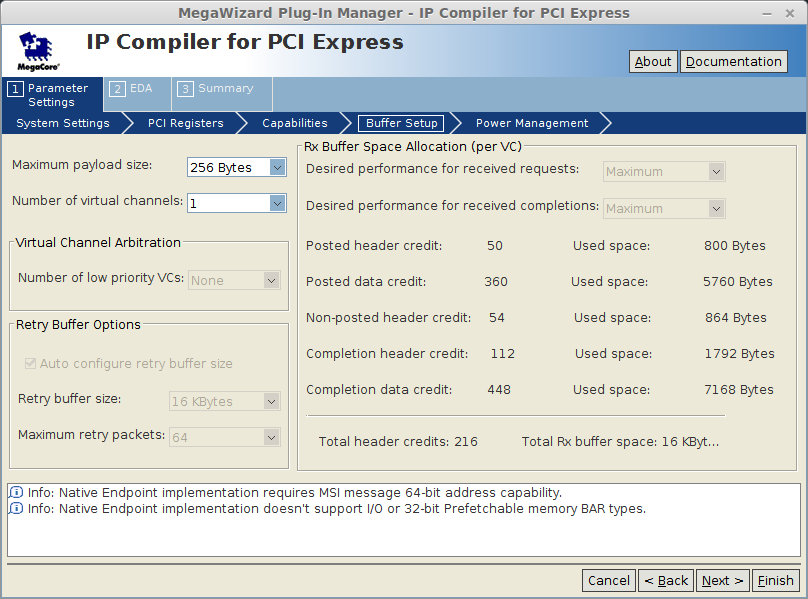
\includegraphics[width=350px,center]{IPCompilerPCIeTabBufferSetup.png}
  \caption{IP Compiler for PCI Express Buffer Setup Tab}
  \label{Fig:Altera:IPCompiler:PCIeBufferSetupTab}
\end{figure}
In Figure~\ref{Fig:Altera:IPCompiler:PCIeBufferSetupTab} select the
\ConfigSetting{Maximum Payload Size} from the dropdown menu. Use this to set the
\RIFFAParameter{C\_MAX\_PAYLOAD} parameter. Set the numer of \ConfigSetting{Virtual Channels} to
\ConfigSetting{1}.

Note: \ConfigSetting{Maximum Payload} sizes are typically set by the BIOS, and
256 bytes seems to be standard. RIFFA will default to the minimum of
\RIFFAParameter{C\_MAX\_PAYLOAD\_SIZE} and the setting in your BIOS. Unless your
BIOS is modified, or can support substantially larger packets, there will be no
performance benefit to increasing the payload size. Increasing the
\ConfigSetting{Maximum Payload} size will increase the resources consumed.

Next, we need to generate the PLL for the example design. Select the ALTPLL
megafunction from the Quartus IP Catalog, to open the window shown in
Figure~\ref{Fig:Altera:ALTPLL:TabGeneral}.
\begin{figure}[H]
  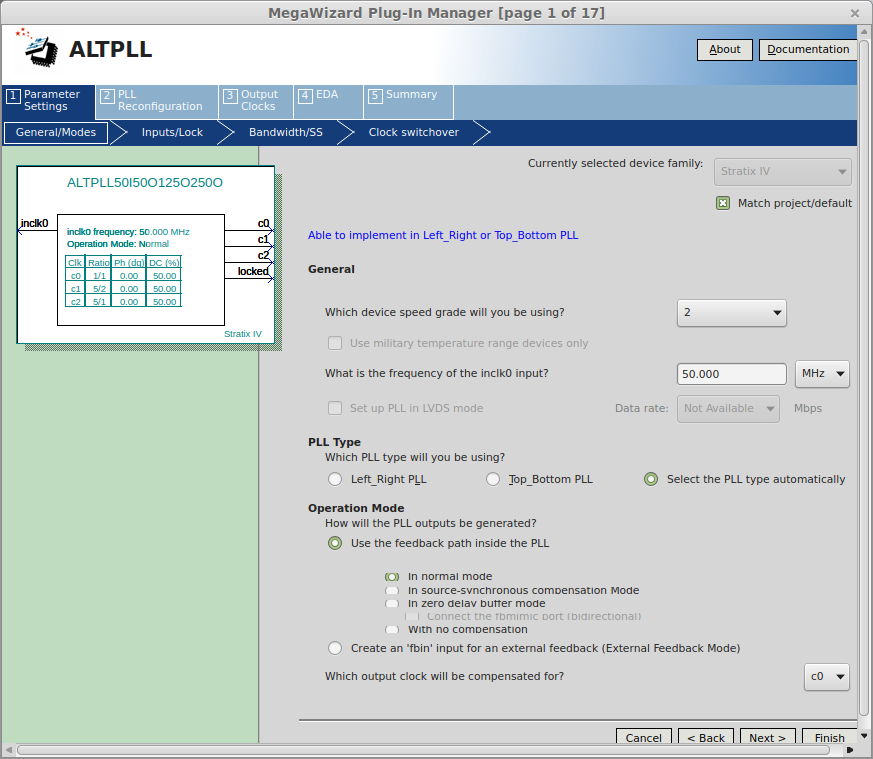
\includegraphics[width=350px,center]{ALTPLLTabGeneral.png}
  \caption{ALTPLL General Settings Tab}
  \label{Fig:Altera:ALTPLL:TabGeneral}
\end{figure}
In Figure~\ref{Fig:Altera:ALTPLL:TabGeneral}, select the \ConfigSetting{Speed
  Grade} that matches your board (Found in the User Guide and online). Next set
the input clock frequency. The DE4 board provides 50 MHz clock inputs and we use
these for convenience. The remaining settings are unchaged. Click on the
Inputs/Lock tab to move on to Figure~\ref{Fig:Altera:ALTPLL:TabInputs}.

Optional: Set the name of the ALTPLL block. In the example designs we use the
name ALTPLL50I50O125O250O, for 50 MHz Input clock, 50, 125, and 250 MHz output
clocks. The 125 and 50 MHz Clocks are required for the PCIe Endpoint.

\begin{figure}[H]
  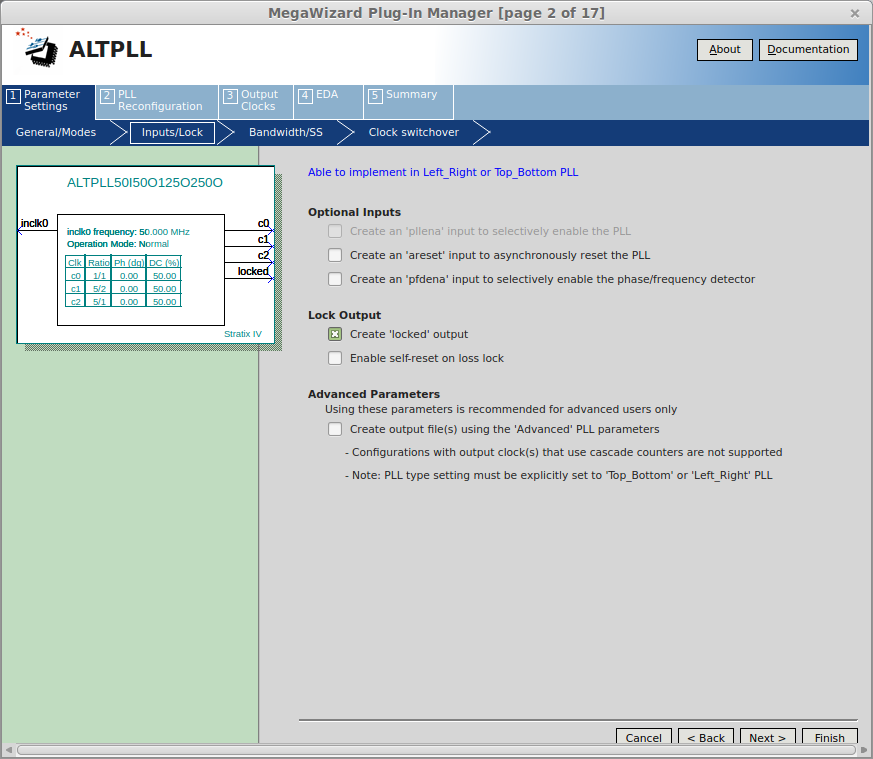
\includegraphics[width=350px,center]{ALTPLLTabInputs.png}
  \caption{ALTPLL Input Settings Tab}
  \label{Fig:Altera:ALTPLL:TabInputs}
\end{figure}
Match the settings shown in Figure~\ref{Fig:Altera:ALTPLL:TabInputs}. In the
Output Clocks Section, create a 50 MHz output clock, 125 MHz clock, and 250 MHz
Clock. Click Finish when done.

% \begin{figure}[H]
%   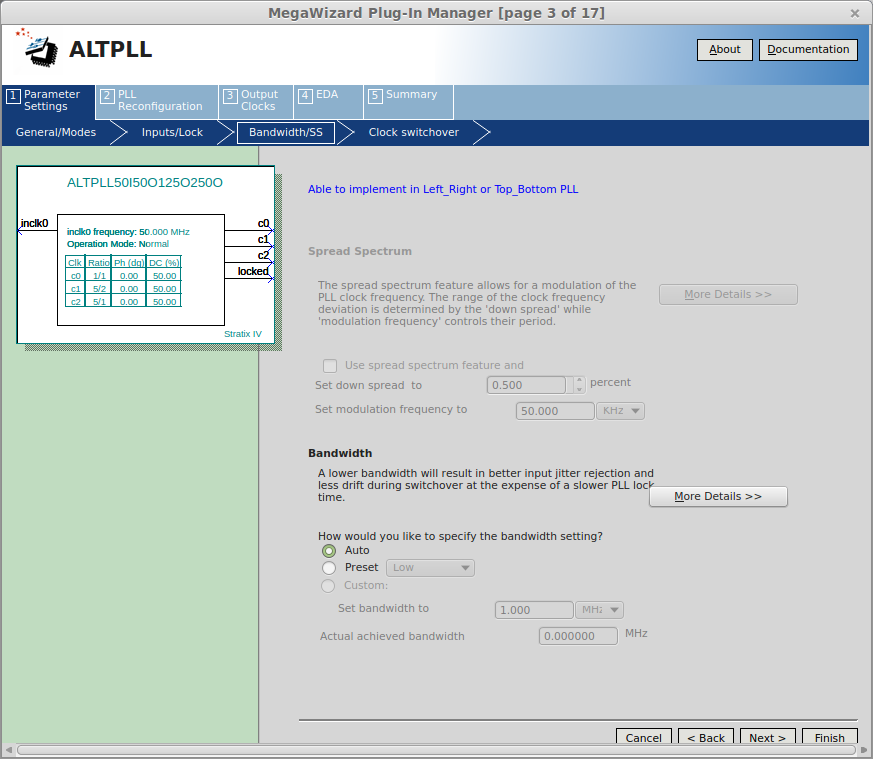
\includegraphics[width=350px,center]{ALTPLLTabBandwidth.png}
%   \caption{ALTPLL Bandwidth Tab}
%   \label{Fig:Altera:ALTPLL:TabBandwidth}
% \end{figure}
% \begin{figure}[H]
%   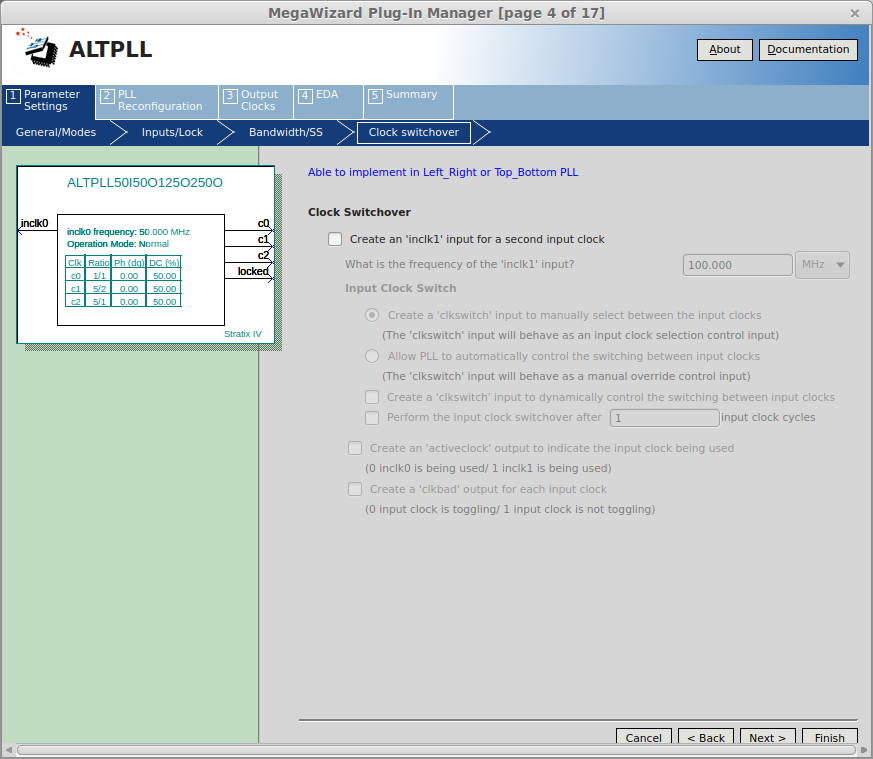
\includegraphics[width=350px,center]{ALTPLLTabSwitchover.png}
%   \caption{ALTPLL Switchover Tab}
%   \label{Fig:Altera:ALTPLL:TabSwitchover}
% \end{figure}

Finally, we generate the ALTGX\_RECONFIG Megafunction. Select the
ALTGX\_RECONFIG megafunction from the Quartus IP Catalog to produce the widown
shown in Figure~\ref{Fig:Altera:ALTGX:TabSettings}.
\begin{figure}[H]
  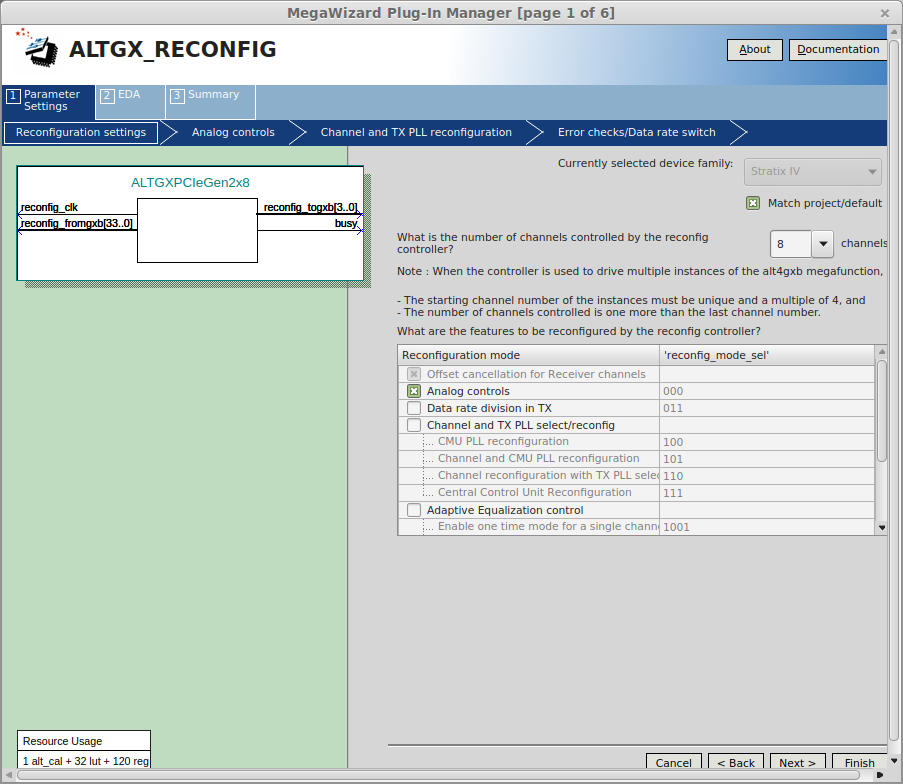
\includegraphics[width=350px,center]{ALTGXReconfigTabSettings.png}
  \caption{ALTGX Reconfiguration Settings Tab}
  \label{Fig:Altera:ALTGX:TabSettings}
\end{figure}
In the Reconfiguration Tab shown in Figure~\ref{Fig:Altera:ALTGX:TabSettings}, set the \ConfigSetting{Number of Channels}. This should be equal to the number of PCIe Lanes at the Top Level. In the Features Section, \ConfigSetting{Enable Analog Controls}. Match the settings in the remaining windows, shown in Figure~\ref{Fig:Altera:ALTGX:TabInputs},Figure~\ref{Fig:Altera:ALTGX:TabChannel}, and Figure~\ref{Fig:Altera:ALTGX:TabError}.

\begin{figure}[H]
  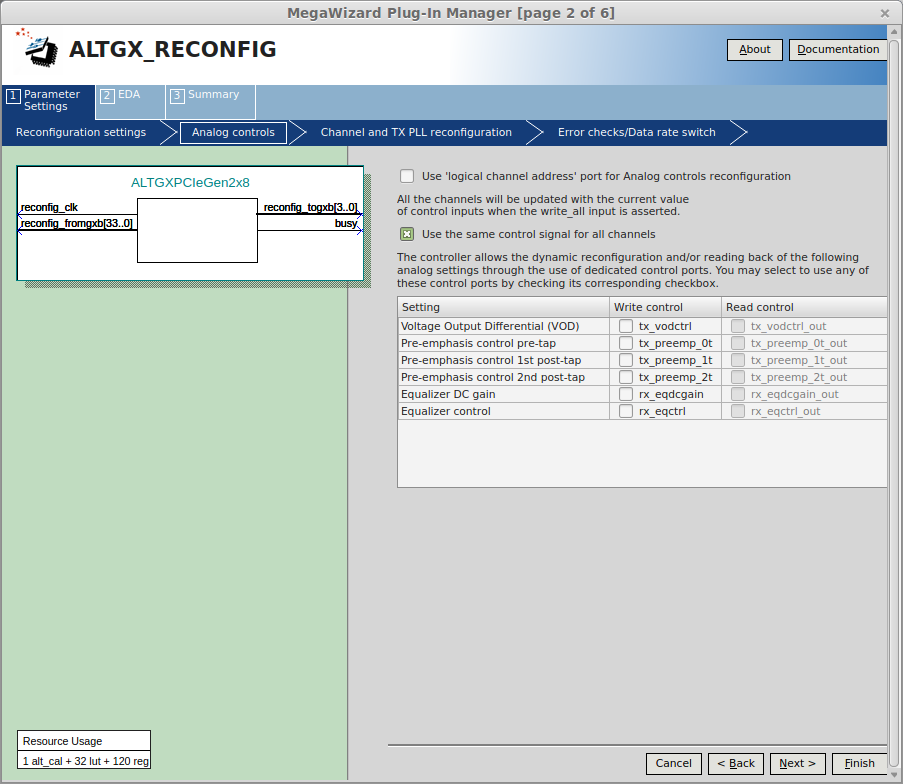
\includegraphics[width=350px,center]{ALTGXReconfigTabAnalog.png}
  \caption{ALTGX Reconfiguration Analog Settings Tab}
  \label{Fig:Altera:ALTGX:TabInputs}
\end{figure}

\begin{figure}[H]
  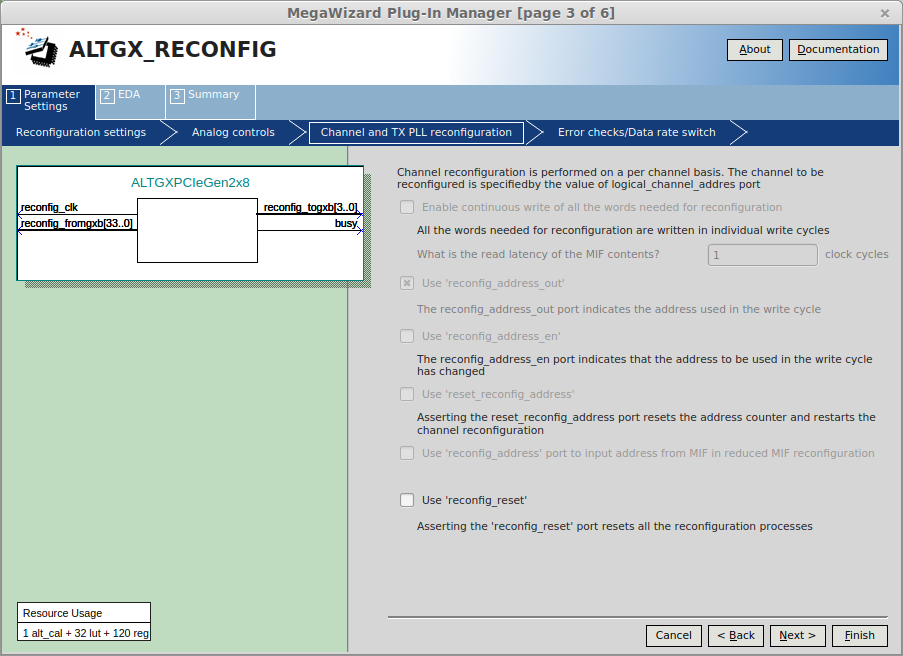
\includegraphics[width=350px,center]{ALTGXReconfigTabChannel.png}
  \caption{ALTGX Reconfiguration Channel Tab}
  \label{Fig:Altera:ALTGX:TabChannel}
\end{figure}

\begin{figure}[H]
  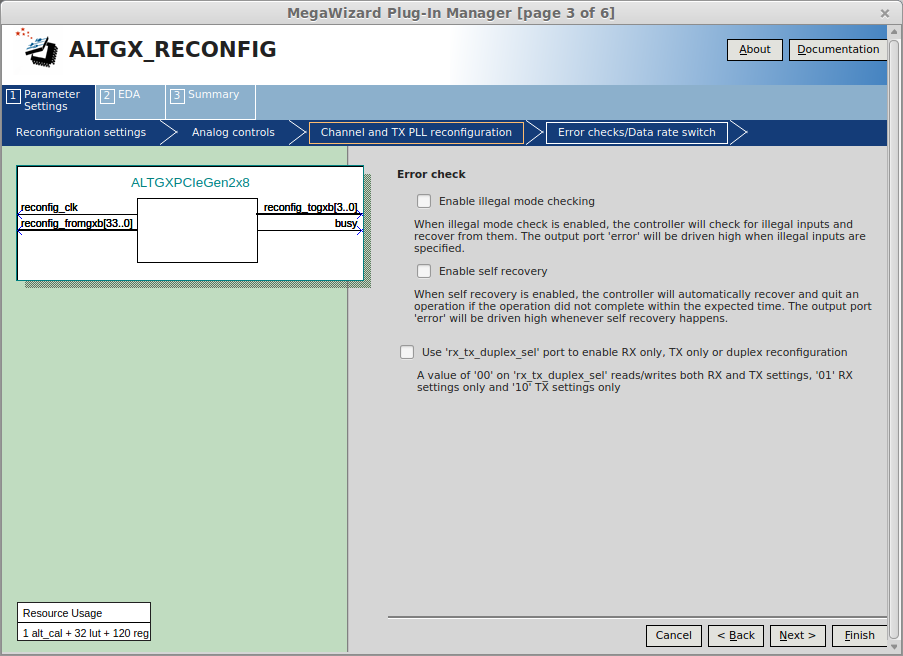
\includegraphics[width=350px,center]{ALTGXReconfigTabError.png}
  \caption{ALTGX Reconfiguration Error Tab}
  \label{Fig:Altera:ALTGX:TabError}
\end{figure}

\pagebreak
\subsection{Creating Constraints files for IP Compiler Designs}
Advanced users may also want to edit and modify the constraint files. This not
required or recommended for novice users. The example designs in the RIFFA
\RIFFAVer~distribution contain appropriate constraint files for the example
designs. However if the need arises, we demonstrate the constraints we used
below.

If the goal is to generate a RIFFA design completely from scratch, each board
directory comes with a RIFFA wrapper verilog file and instantiates a
vendor-specific translation layer. It is highly recommended to re-use these
files RIFFA wrapper when creating designs from scratch. Users should also use
the constraints file (\Altera{.sdc}) in the board directory, and in the
\Directory{constr/}, or read the User Guide provided with each board.

To appropriately constrain your PCIe reference clocks, place the constraints
shown in Listing~\ref{Listing:Altera:IPCompiler:Constraints} in your
\Altera{.sdc} file. Modify the name of the osc\_50MHz and PCIE\_REFCLK ports to
match your design
\begin{lstlisting}[language=tcl,basicstyle=\footnotesize\ttfamily,commentstyle=\color{red},
    label=Listing:Altera:IPCompiler:Constraints,
    caption=\Altera{.sdc} constraints for Qsys and Megawizard designs,frame=single]
  create_clock -name PCIE_REFCLK -period 10.000 [get_ports {PCIE_REFCLK}]
  create_clock -name osc_50MHz -period 20.000 [get_ports {OSC_BANK3D_50MHZ}]
  derive_pll_clocks -create_base_clocks
  derive_clock_uncertainty
  # 50 MHZ PLL Clock
  create_generated_clock -name clk50 -source [get_ports {OSC_50_BANK2}] \
  [get_nets {*|altpll_component|auto_generated|wire_pll1_clk[0]}]
  # 125 MHZ PLL Clock
  create_generated_clock -name clk125 -multiply_by 5 -divide_by 2 -source \
  [get_ports {OSC_50_BANK2}] \
  [get_nets {*|altpll_component|auto_generated|wire_pll1_clk[1]}]
  # 250 MHZ PLL Clock
  create_generated_clock -name clk250 -multiply_by 5 \ 
  -source [get_ports {OSC_50_BANK2}] [get_nets \
    {*|altpll_component|auto_generated|wire_pll1_clk[2]}]
\end{lstlisting}

Likewise, copy the constraints in
Listing~\ref{Listing:Altera:IPCompiler:QSFSettings} into your \Altera{.qsf}
file. Copy the location assignment commands for each PCIe Pin in your reference
design.
\begin{lstlisting}[language=tcl,basicstyle=\footnotesize\ttfamily,
    commentstyle=\color{red},label=Listing:Altera:IPCompiler:QSFSettings,
    caption=\Altera{.qsf} settings for IP Compiler Designs,frame=single]
  ###################################################################
  # PCIE Connections
  ###################################################################
  set_location_assignment <PCIE_REFCLK_PIN> -to PCIE_REFCLK
  set_instance_assignment -name IO_STANDARD HCSL -to PCIE_REFCLK
  set_location_assignment <PCIE_REFCLK_PIN(n)> -to ``PCIE_REFCLK(n)''
  set_instance_assignment -name IO_STANDARD HCSL -to ``PCIE_REFCLK(n)''
  set_location_assignment <PCIE_RESET_N> -to PCIE_RESET_N
  set_instance_assignment -name IO_STANDARD ``2.5 V'' -to PCIE_RESET_N

  # For each PCIE Lane (L) set the pin locations from the board user guide!
  ######################################################################
  #PCIE TX_OUT L
  ######################################################################
  set_location_assignment <TX_LANE[L]_PIN>   -to PCIE_TX_OUT[L]
  set_location_assignment <TX_LANE[L]_PIN(n)> -to ``PCIE_TX_OUT[L](n)''
  ###################################################################
  #PCIE RX_IN L
  ###################################################################
  set_location_assignment <RX_LANE[L]_PIN>  -to PCIE_RX_IN[L]
  set_location_assignment <RX_LANE[L]_PIN(n)> -to ``PCIE_RX_IN[L](n)''
\end{lstlisting}
\pagebreak
\chapter{Developer Documentation}
This chapter describes RIFFA \RIFFAVer~at a level of detail that is useful for
RIFFA developers. Users of RIFFA should not read this section until they are
comfortable developing for RIFFA or have experience with PCIe and DMA
concepts. 
\section{Architecture Description}
\begin{figure}[H]
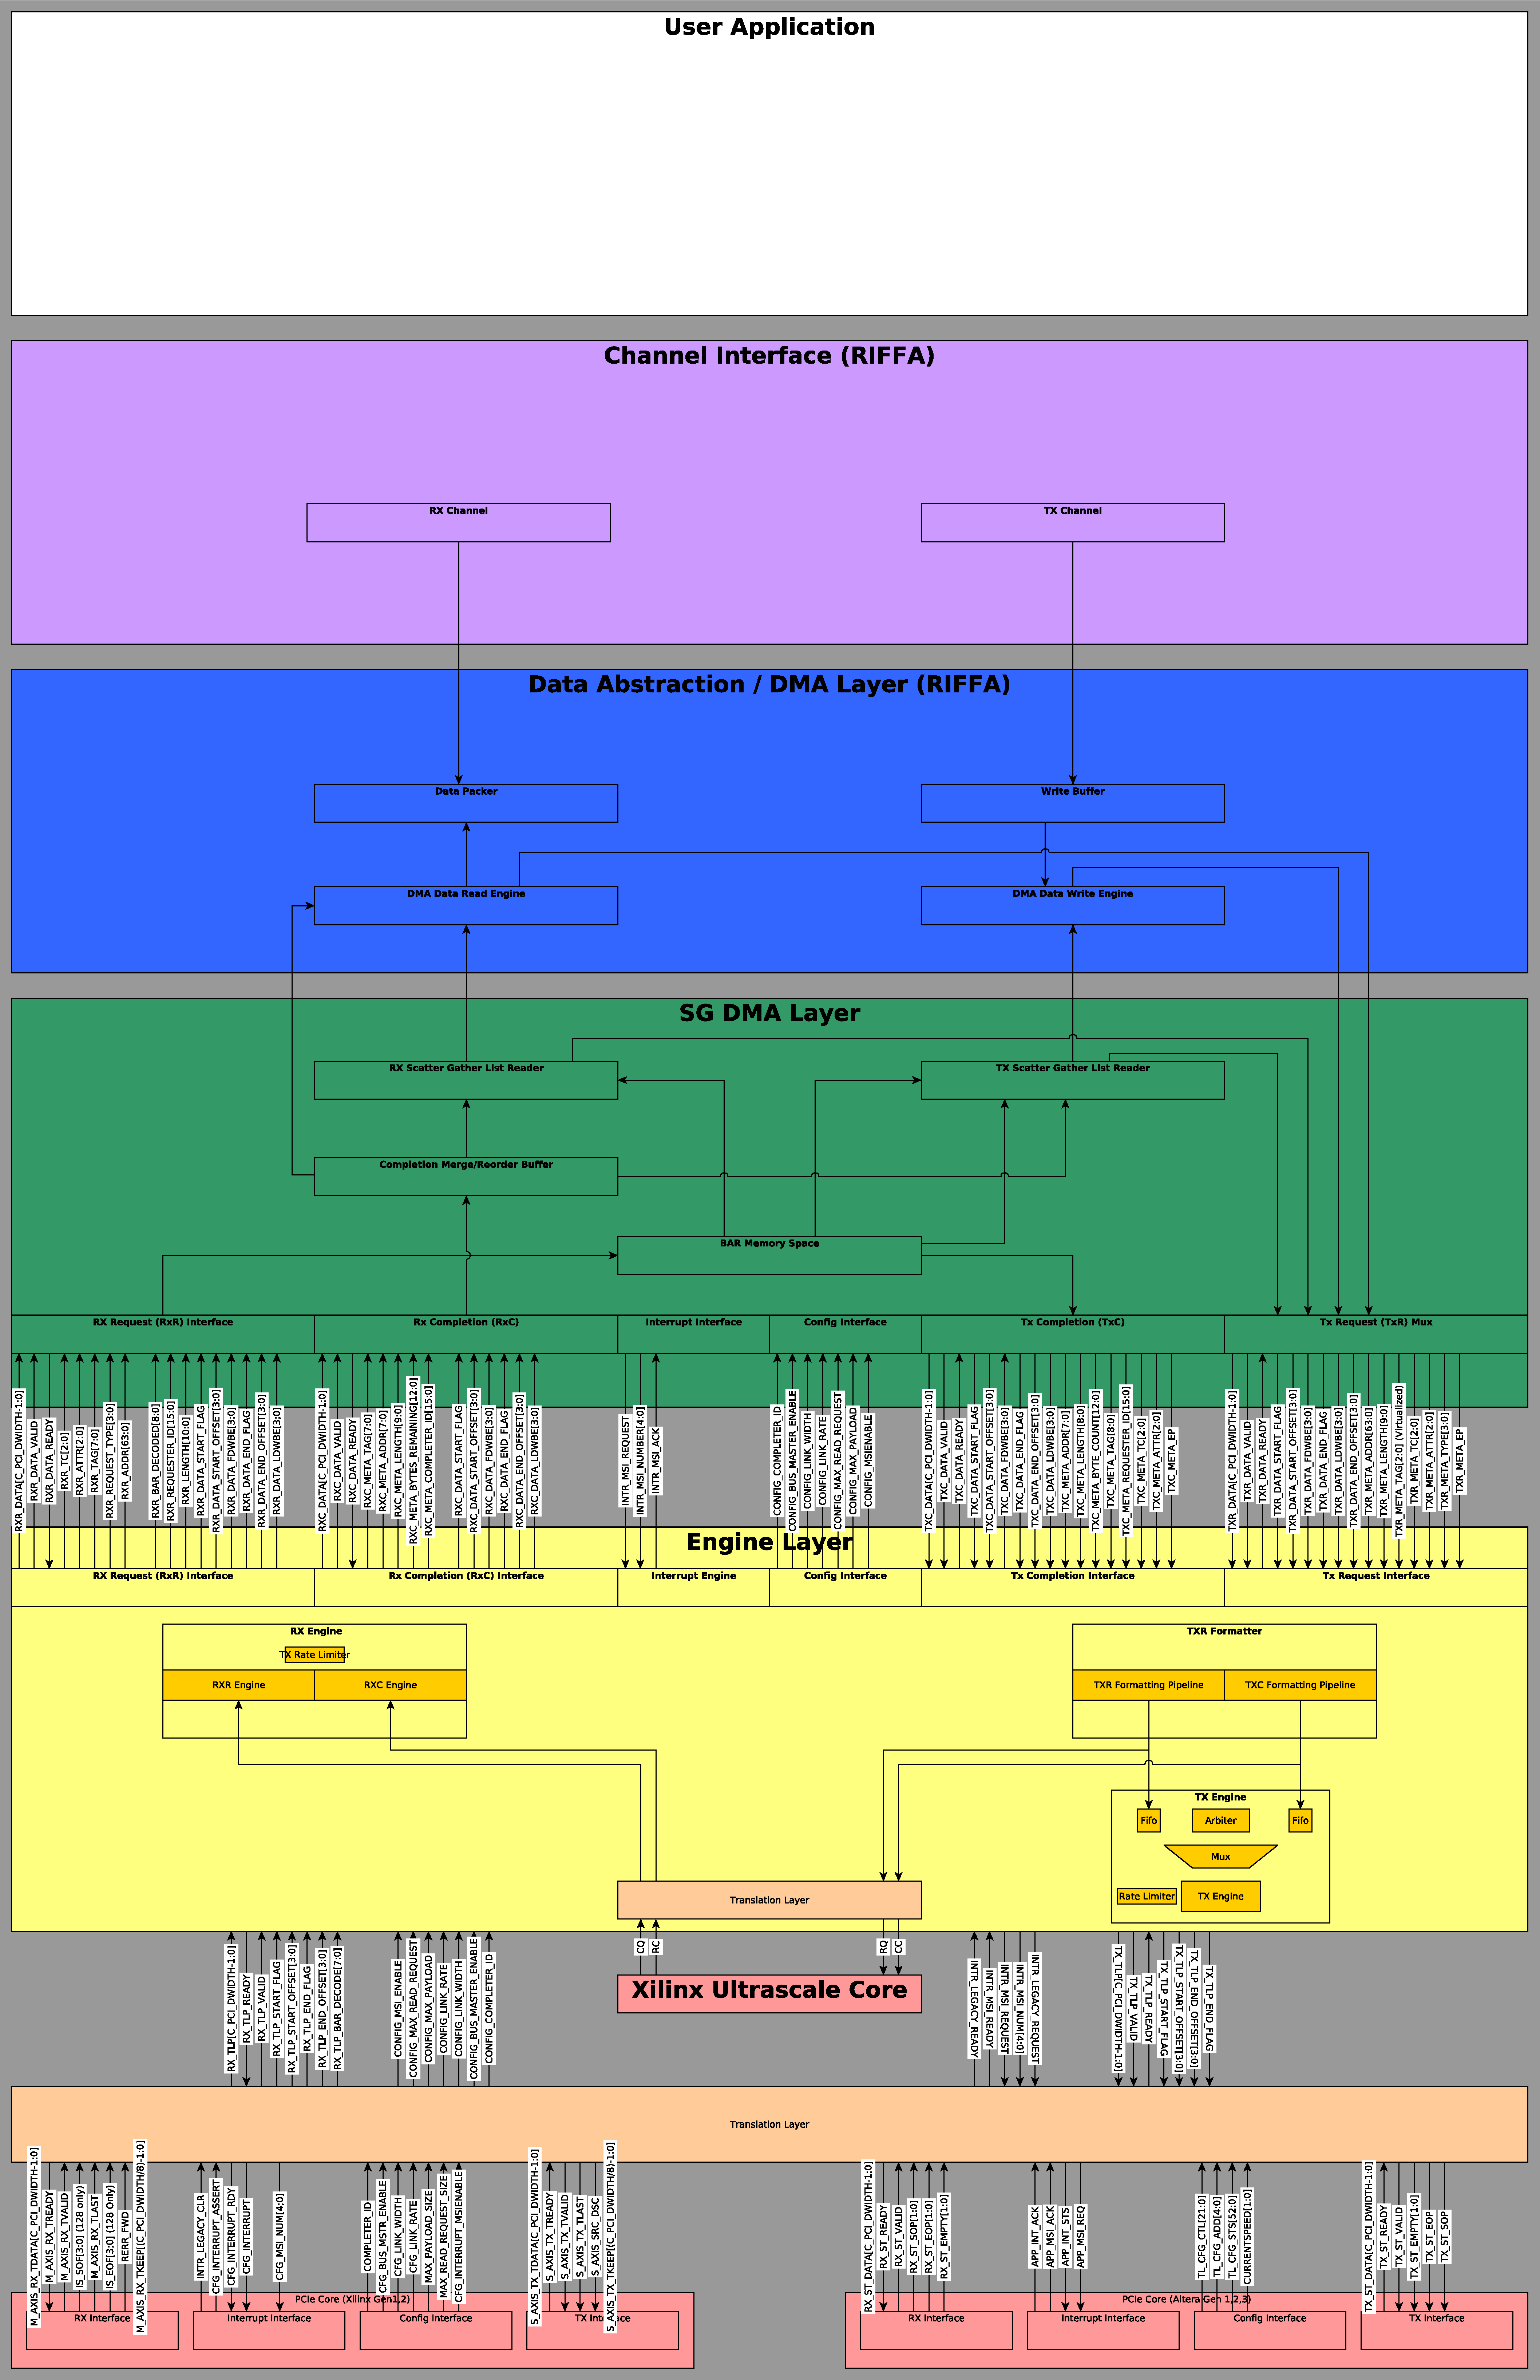
\includegraphics[width=350px,center]{RIFFA.pdf}
  \caption{High level RIFFA Diagram}
  \label{Fig:Developer:HighLevel:Full}
\end{figure}
\begin{itemize}
\item \textbf{\color{red}{IP Interfaces}} The Vendor IP interfaces provied
  low-level access to the PCIe bus. Each vendor provides a set of signals for
  communicating over PCIe. Xilinx FPGAs without PCIe Gen3 support provide an
  interface very similar to Altera FPGAs. We call this the ``Classic
  Interface''. Newer Xilinx devices with PCIe Gen3 support have completely
  different non-compatible interfaces (CC, CQ, RC, RQ instead of RX and TX). We
  call this the ``Xilinx Ultrascale Interface''.

  \textit{Files: \Xilinx{*.xci}, \Altera{*.qsys} (And others generated by vendor
    tools)}

\item \textbf{\color{orange}{Translation Layer}} The Translation Layer provides
  a set of vendor-independent interfaces and signal names. 

  There is one translation layer for each interface. The ``Classic Translation
  Layer'' provides a set of interfaces (RX, TX, Interrupt, and Configuration)
  and vendor independent signal names to higher layers. There is very little
  logic in these layers, and there should be no timing-critical logic here.

  The ``Ultrascale Translation Layer'' operates on the ultrascale
  interface. Similar to the classic translation layer, it contains very little
  logic. It provides the interfaces: RX Completion, RX Request, TX
  Completion, TX Request, Interrupt, and Configuration. 

  \textit{Files: translation\_altera.v, translation\_xilinx.v,
    txc\_engine\_ultrascale.v,\\ txr\_engine\_ultrascale.v}

\item \textbf{\color{yellow}{Formatting Engine Layer}} The Formatting Engine
  Layer is responsible for formatting requests and completions into
  packets. This layer provides four interfaces: RX Completion (RXC) for
  receiving completions (responses to memory read requests), RX Request (RXR)
  for receiving memory read and write requests, TX Completion (TXC) for
  transmitting completions (reponses to memory read requests), and TX Request
  (TXR) for transmitting read and write requests.
  
  The engine layer abstracts vendor specific features, such as Xilinx's
  Classic-Interface Big-Endian requirement and Altera's Quad-word
  Alignment. The C\_VENDOR parameter for the engine layer switches between
  Xilinx, Altera, and Ultrascale logic to produce TLPs (Classic Interface) and
  AXI Descriptors (Ultrascale Interface).

  The RX path of the engine layer has packet parsers for TLPs and AXI
  Descriptors. These are parameterized by width, as of RIFFA 2.2. The TX Path of
  the engine layer has packet formatters for TLPs and AXI Descriptors. 

  As alluded to in the Translation Layer, the Classic IP Cores provide only two
  transmit interfaces (RX, and TX), while the Xilinx Ultrascale IP Core handles
  RX Demultiplexing and multiplexing internally and provides four interfaces
  (RXC, RXR, TXC, and TXR). For this reason, the multiplexing/FIFO logic used in
  the Classic interfaces are not necessary for the Xilinx interface.

  After the Engine-Layer, higher layers should be vendor agnostic, if not bus
  agnostic. The exception will be sideband signals signals. (How much of this
  ideal can be achieved remains to be seen)

  Note: The engine layer currently uses word-aligned addresses, and byte-enable
  signals to specify sub-word addresses. In the future, all addresses will be
  byte-aligned and word enables will be handled in the formatting logic. 

  \textit{Files: engine\_layer.v, schedules.vh, rx\_engine\_classic.v, rxc\_engine\_classic.v,\\
    rxr\_engine\_classic.v, tx\_engine\_classic.v, txc\_engine\_classic.v,\\
    txr\_engine\_classic.v, rx\_engine\_ultrascale.v, rxc\_engine\_ultrascale.v,\\
    rxr\_engine\_ultrascale.v, tx\_engine\_ultrascale.v, txc\_engine\_ultrascale.v, \\
    txr\_engine\_ultrascale.v}
   
\item \textbf{\color{green}{Scatter Gather (SG) DMA Layer}} The Scatter Gather
  DMA Layer handles reading from and writing to scatter gather lists and
  providing the addresses found in these lists to the data-request logic in the
  Data Abstraction layer. In RIFFA, each channel has its own SG DMA list logic.

  The Completion Merge/Reorder buffer handles out-of-order completions. In the
  PCIe specification, a memory request can be serviced by multiple smaller
  completions (the responses must remain in order). Completions from different
  memory requests can be returned in any order. The reorder buffer releases data
  when all of the responses to a memory request have been received.

  Memory read and write requests to the host are multiplexed by the TX Request
  Mux. These are serviced fairly in round robin order.
  
  The Scatter Gather List Readers issue read requests to read data from the
  Scatter Gather List (SGL) created by the driver. This list contains the
  address and length of pages containing data to transmit. When an SGL has been
  exhausted, an interrupt is raised and the SGL is refilled or the transaction
  is comlete.

  Each element in the SGL 128-bit triple: {32'b0, 32'b Length of Data in 32-bit
    words, 64'b Address of Page}. The addresses in this list are provided to the
  DMA Data Read Engine in the Data Abstraction layer. Since the SGL must be a
  single continuous stream of 128-bit elements regardless of the size of the
  interface, gaps and mis-alignments due to packet formatting are removed using
  the Data Packer, which receives its data from the reorder buffer.
  
  The location of the SGL in host memory is written to the BAR Memory space.
  The BAR Memory space is partitioned among the channels. Only the host can
  issue read and write requests to this memory space. Since the memory space is
  partitioned, the RX Request interface and TX Completion interface do not have
  demultiplexing or multiplexing logic.

  A more through treatment of the SG DMA Layer can be found in Sec.~\ref{Sec:Developer:Arch:SGDMA}.

  \textit{Files: reorder\_queue*.v, sg\_list\_reader\_*.v, sg\_list\_requester.v \\ 
    fifo\_packer\_*.v, registers.v, tx\_multiplexer\_*.v}


\item \textbf{\color{blue}{Data Abstraction / DMA Layer}} The Data Abstraction /
  DMA Layer is responsible for making requests to read data from, or write data
  to host memory.

  The read and write addresses are provided by the Scatter Gather list
  readers. Since RIFFA provides a single continuous stream of 32-bit words
  regardless of the size of the interface, gaps and mis-alignments due to packet
  formatting are removed using the Data Packer, which receives its data from the
  reorder buffer. On the TX side, this is not necessary. However a write buffer,
  and other transaction tracking logic is necessary for buffering, and removing
  non-integral data.

  A more through treatment of the Data Abstraction Layer can be found in
  Sec.~\ref{Sec:Developer:Arch:DataAbstraction}.

  \textit{Files: reorder\_queue*.v, rx\_port\_*.v, rx\_port\_reader.v,\\
    fifo\_packer\_*.v, tx\_port\_writer.v tx\_port\_buffer\_*.v tx\_port\_monitor\_*.v}

\item \textbf{\color{purple}{Channel Interface}}
  \textit{Files: rx\_channel\_gate\_*.v, tx\_channel\_gate\_*.v}
\contourlength{.2pt}
\item \contour{black}{\textbf{\color{white}{User Logic}}}
\end{itemize}
\subsection{Scatter Gather DMA Layer}
\label{Sec:Developer:Arch:SGDMA}
READS from the SG lists are prioritized
\subsection{Data Abstraction DMA Layer}
\label{Sec:Developer:Arch:DataAbstraction}
\section{Software Description}

\section{FPGA RX Transfer / Host Send}
\begin{center}
  \begin{tabular}{ | l | l |}
    \hline
    Parameter & Value \\ \hline
    Data Transfer Length & 128 (32-bit words)\\ \hline
    Data Transfer Offsfet & 0\\ \hline
    Data Transfer Last & 1\\ \hline
    Data Transfer Channel & 0\\ \hline
    Data Page Address (DMA) & 0x00000000\_FEED0000\\ \hline
    SGL Head Address & 0x00000000\_BEEF0000\\ \hline
  \end{tabular}
\end{center}

\begin{itemize}
 \item A user makes an call to fpga\_send() to transfer 128 32-bit words of data on Channel 0.  \item The RIFFA driver writes \{32'd128\} to Channel 0's RX Length register, and
   \{31'd0,1'b1\} to Channel 0's RX OffLast register. This notifies the FPGA that a new
   transfer is happening and will raise CHNL\_RX for the user
   application. \textit{Files: rxr\_engine\_*.v, registers.v, channel*.v,
     rx\_port.v rx\_port\_gate.v, rx\_port\_reader.v}
 \item The RIFFA driver allocates an SGL with 1 element (4 32-bit words) at
   address \\\{64'h0000\_0000\_BEEF\_0000\}. The driver fills the list with the
   length and address of the user data:\\
    \{32'd0,32'd128,64'h0000\_0000\_FEED\_0000\}.
 \item The RIFFA driver communicates the address and length of the SGL by
   writing \\\{32'hBEEF0000\} to to Channel 0's RX SGL Address Low register,
   \{32'd0\} to to Channel 0's RX SGL Address High register, and \{32'd4\} to to
   Channel 0's RX SGL Length register. Writing the RX SGL Length register
   notifies the RX SG Engine that a transfer has started, and the low and high
   portions of the 64-bit RX SGL Address are valid. \textit{Files:
     rxr\_engine\_*.v, registers.v, channel*.v, rx\_port.v,
     sg\_list\_requester.v}
 \item The SG List Requester on the FPGA issues a read request for 4 32-bit
   words of data starting at address 0xBEEF0000. The FPGA also issues an
   interrupt. The RIFFA driver reads the Interrupt Status Register of the FPGA
   and determines that Channel 0 has finished reading the RX SGL. \textit{Files:
     sg\_list\_requester.v, rx\_port\_requester\_mux.v, rx\_port\_*.v,
     channel*.v, tx\_multiplexer.v, engine\_layer.v, txr\_engine\_*.v,
     interrupt.v}
 \item The FPGA receieves a completion with 4 32-bit words. After being enqueued
   in the reorder buffer, the completion is delivered to Channel 0, and packed
   into the SGL RX Fifo. \textit{Files: rxc\_engine\_*.v, engine\_layer.v,
     reorder\_queue*.v, fifo\_packer\_*.v}
 \item The RX Port Reader removes the SG element from the FIFO, and issues
   several read requests to receive all 128 32-bit words. \textit{Files:
     rx\_port\_reader.v, rx\_port\_*.v, channel*.v, tx\_multiplexer.v,
     engine\_layer.v, txr\_engine\_*.v, tx\_multiplexer.v}
 \item The completions return interleaved and are reordered in the reorder
   buffer. The reorder buffer releases the completions in order to the fifo
   packer, which puts them in the FIFO. The RX Port Channel Gate issues the data
   to the user. \textit{Files: rxc\_engine\_*.v, engine\_layer.v, reorder\_queue*.v,
     fifo\_packer\_*.v, rx\_port\_reader.v, rx\_port\_channel\_gate.v, channel*.v}
\item The FPGA raises an interrupt with the last word of data is put into the
  Main Data Fifo. The RIFFA driver reads the Interrupt Status Register of the
  FPGA and determines that Channel 0 has finished the RX Transaction. The RIFFA
  driver reads the RX Words Read register to determine how many words were read
  during the transaction.
\item Control is returned to the user.
\end{itemize}
\section{TX Transfer}
\section{FPGA RX Transfer / Host Send}
\begin{center}
  \begin{tabular}{ | l | l |}
    \hline
    Parameter & Value \\ \hline
    Data Transfer Length & 128 (32-bit words)\\ \hline
    Data Transfer Offsfet & 0\\ \hline
    Data Transfer Last & 1\\ \hline
    Data Transfer Channel & 0\\ \hline
    Data Page Address (DMA) & 0x00000000\_FEED0000\\ \hline
    SGL Head Address & 0x00000000\_BEEF0000\\ \hline
  \end{tabular}
\end{center}
\begin{itemize}
 \item A user makes an call to fpga\_recv() to transfer 128 32-bit words of data
   from Channel 0.
 \item The RIFFA driver allocates an SGL with 1 element (4 32-bit words) at
   address\\ \{64'h0000\_0000\_BEEF\_0000\}. The driver fills the list with the
   length and address of the user data:
    \{32'd0,32'd128,64'h0000\_0000\_FEED\_0000\}.
  \item The user application independently raises CHNL\_TX and starts writing data to\\
    CHNL\_TX\_DATA. RIFFA core logic reads transaction parameters from
    CHNL\_TX\_OFF, CHNL\_TX\_LAST, and CHNL\_TX\_LEN and acknowledges them with
    CHNL\_TX\_ACK. \\\textit{Files: tx\_port\_channel\_gate.v}
  \item An interrupt is raised by the FPGA. The RIFFA driver reads the Interrupt
    Status Register of the FPGA and determines that Channel 0 wishes to start a
    new TX Transaction. The driver ISR reads \{32'd128\} from Channel 0's TX
    Length register, and \{31'd0, 1'b1\} from Channel 0's TX OffLast
    register. Reading the OffLast register notifies the FPGA that the new
    transfer has been accepted. \textit{Files: rxr\_engine\_*.v, riffa.v,
      registers.v, channel*.v, tx\_port\_*.v, tx\_port\_writer.v,
      tx\_port\_monitor\_*.v, engine\_layer.v, txc\_engine\_*.v}
 \item The RIFFA driver communicates the address and length of the SGL by
   writing\\ \{32'hBEEF\_0000\} to to Channel 0's TX SGL Address Low register,
   \{32'd0\} to to Channel 0's TX SGL Address High register, and \{32'd4\} to to
   Channel 0's TX SGL Length register. Writing the TX SGL Length register
   notifies the TX SG Engine that a transfer has started, and the low and high
   portions of the 64-bit TX SGL Address are valid. \textit{Files:
     rxr\_engine\_*.v, registers.v, channel*.v, rx\_port.v,
     sg\_list\_requester.v}
 \item The SG List Requester on the FPGA issues a read request for 4 32-bit
   words of data starting at address 0xBEEF0000. The FPGA raises an
   interrupt. The RIFFA driver reads the Interrupt Status Register of the FPGA
   and determines that Channel 0 has finished reading the TX SGL. \textit{Files:
     sg\_list\_requester.v, rx\_port\_requester\_mux.v, rx\_port\_*.v,
     channel*.v, tx\_multiplexer.v, engine\_layer.v, txr\_engine\_*.v,
     interrupt.v}
 \item The FPGA receieves a completion with 4 32-bit words. After being enqueued
   in the reorder buffer, the completion is delivered to Channel 0, and packed
   into the SGL TX Fifo. \textit{Files: rxc\_engine\_*.v, engine\_layer.v,
     reorder\_queue*.v, fifo\_packer\_*.v}
 \item The TX Port Writer removes the SG element from the FIFO, and issues
   several write requests to write all 128 32-bit words. \textit{Files:
     tx\_port\_monitor.v, tx\_port\_writer.v, tx\_port\_*.v, channel*.v, tx\_multiplexer.v,
     engine\_layer.v, txr\_engine\_*.v, tx\_multiplexer.v}
 \item When the last write transaction has been accepted by the core, the FPGA
   raises an interrupt. The RIFFA driver reads the Interrupt Status Register of
   the FPGA and determines that Channel 0 has finished writing data. The RIFFA
   driver reads the TX Words Written register to determine how many words were
   written during the transaction (in case of early termination, or overflow).
   \textit{Files: rxr\_engine\_*.v, riffa.v, interrupt.v, registers.v, channel*.v,
     tx\_port\_*.v, tx\_port\_writer.v, engine\_layer.v, txc\_engine\_*.v}
 \item Control is return to the user because the TX\_LAST signal was set to 1.
\end{itemize}
%\pagebreak
%\chapter{The RIFFA Architecture}
%\section{Translation Layer}
%\section{Engine Layer}
%\section{DMA Layer}
%\section{RIFFA}
%\section{The DMA Engine Layer}
%\chapter{Version Notes}
%\section{References, Notes and Reading Material}
%\section{Core Diagrams}
\end{document}
